% Copyright (C) 2014-2017 by Thomas Auzinger <thomas@auzinger.name>

\documentclass[draft, final]{vutinfth} % Remove option 'final' to obtain debug information.

% Load packages to allow in- and output of non-ASCII characters.
\usepackage{lmodern}        % Use an extension of the original Computer Modern font to minimize the use of bitmapped letters.
\usepackage[T1]{fontenc}    % Determines font encoding of the output. Font packages have to be included before this line.
\usepackage[utf8]{inputenc} % Determines encoding of the input. All input files have to use UTF8 encoding.

% Extended LaTeX functionality is enables by including packages with \usepackage{...}.
\usepackage{amsmath}    % Extended typesetting of mathematical expression.
\usepackage{amssymb}    % Provides a multitude of mathematical symbols.
\usepackage{mathtools}  % Further extensions of mathematical typesetting.
\usepackage{microtype}  % Small-scale typographic enhancements.
\usepackage[inline]{enumitem} % User control over the layout of lists (itemize, enumerate, description).
\usepackage{multirow}   % Allows table elements to span several rows.
\usepackage{booktabs}   % Improves the typesettings of tables.
%\usepackage{subcaption} % Allows the use of subfigures and enables their referencing.
\usepackage{subfig}
\usepackage[ruled,linesnumbered,algochapter]{algorithm2e} % Enables the writing of pseudo code.
\usepackage[usenames,dvipsnames,table]{xcolor} % Allows the definition and use of colors. This package has to be included before tikz.
\usepackage{nag}       % Issues warnings when best practices in writing LaTeX documents are violated.
\usepackage{todonotes} % Provides tooltip-like todo notes.
\usepackage{hyperref}  % Enables cross linking in the electronic document version. This package has to be included second to last.
\usepackage[acronym,toc]{glossaries} % Enables the generation of glossaries and lists fo acronyms. This package has to be included last.
\usepackage{cleveref}
\usepackage{svg}
\usepackage{bm}

% Define convenience functions to use the author name and the thesis title in the PDF document properties.
\newcommand{\authorname}{Tanja Šarčević} % The author name without titles.
\newcommand{\thesistitle}{Fingerprinting Relational Databases} % The title of the thesis. The English version should be used, if it exists.
\newcommand{\thesissubtitle}{Quality Evaluation and Impact on Learning Tasks}

% Set PDF document properties
\hypersetup{
    pdfpagelayout   = TwoPageRight,           % How the document is shown in PDF viewers (optional).
    linkbordercolor = {Melon},                % The color of the borders of boxes around crosslinks (optional).
    pdfauthor       = {\authorname},          % The author's name in the document properties (optional).
    pdftitle        = {\thesistitle},         % The document's title in the document properties (optional).
    pdfsubject      = {Subject},              % The document's subject in the document properties (optional).
    pdfkeywords     = {a, list, of, keywords} % The document's keywords in the document properties (optional).
}

\setpnumwidth{2.5em}        % Avoid overfull hboxes in the table of contents (see memoir manual).
\setsecnumdepth{subsection} % Enumerate subsections.

\nonzeroparskip             % Create space between paragraphs (optional).
\setlength{\parindent}{0pt} % Remove paragraph identation (optional).

\makeindex      % Use an optional index.
\makeglossaries % Use an optional glossary.
%\glstocfalse   % Remove the glossaries from the table of contents.

% Set persons with 4 arguments:
%  {title before name}{name}{title after name}{gender}
%  where both titles are optional (i.e. can be given as empty brackets {}).
\setauthor{}{\authorname}{}{female}
\setadvisor{Ao.Univ.Prof. Dipl.-Ing. Dr.techn.}{Andreas Rauber}{}{male}

% For bachelor and master theses:
\setfirstassistant{Mag.rer.soc.oec. Dipl.-Ing.}{Rudolf Mayer}{}{male}
%\setsecondassistant{Pretitle}{Forename Surname}{Posttitle}{male}
%\setthirdassistant{Pretitle}{Forename Surname}{Posttitle}{male}

% For dissertations:
\setfirstreviewer{Pretitle}{Forename Surname}{Posttitle}{male}
\setsecondreviewer{Pretitle}{Forename Surname}{Posttitle}{male}

% For dissertations at the PhD School and optionally for dissertations:
\setsecondadvisor{Pretitle}{Forename Surname}{Posttitle}{male} % Comment to remove.

% Required data.
\setaddress{Schäffergasse 2/418, 1040 Vienna, Austria}
\setregnumber{01640006}
\setdate{04}{09}{2019} % Set date with 3 arguments: {day}{month}{year}.
\settitle{\thesistitle}{Fingerprinting Relational Databases} % Sets English and German version of the title (both can be English or German). If your title contains commas, enclose it with additional curvy brackets (i.e., {{your title}}) or define it as a macro as done with \thesistitle.
\setsubtitle{Quality Evaluation and Impact on Learning Tasks}{Quality Evaluation and Impact on Learning Tasks} % Sets English and German version of the subtitle (both can be English or German).

% Select the thesis type: bachelor / master / doctor / phd-school.
% Bachelor:
%\setthesis{bachelor}
%
% Master:
\setthesis{master}
\setmasterdegree{dipl.} % dipl. / rer.nat. / rer.soc.oec. / master
%
% Doctor:
%\setthesis{doctor}
%\setdoctordegree{rer.soc.oec.}% rer.nat. / techn. / rer.soc.oec.
%
% Doctor at the PhD School
%\setthesis{phd-school} % Deactivate non-English title pages (see below)

% For bachelor and master:
\setcurriculum{Logic and Computation}{Logic and Computation} % Sets the English and German name of the curriculum.

% For dissertations at the PhD School:
%\setfirstreviewerdata{Affiliation, Country}
%\setsecondreviewerdata{Affiliation, Country}


\begin{document}

\frontmatter % Switches to roman numbering.
% The structure of the thesis has to conform to
%  http://www.informatik.tuwien.ac.at/dekanat

\addtitlepage{naustrian} % German title page (not for dissertations at the PhD School).
\addtitlepage{english} % English title page.
\addstatementpage

%\begin{danksagung*}
%\todo{Ihr Text hier.}
%\end{danksagung*}

\begin{acknowledgements*}
I thank my parents for giving me unconditional and unlimited support, love and understanding through the years of my education. I thank them for teaching me the importance of hard work and constant learning. Without them and their set of values, which they have been so tirelessly passing on to me, this thesis would not be possible.

I thank my brother, my grandparents and the rest of my family for their patience, support and valuable advice. 

I express my sincere gratitude to my advisor, Rudolf Mayer, for his time, guidance, cooperation and patience during the process of writing this thesis. His encouragement helped me, not only during the period of writing the thesis but in academic progress in general, as well. Many thanks to my supervisor, prof. Andreas Rauber, for his help and support.

I would like to acknowledge all of my friends that shared with me the journey from the very beginnings of my master studies until this moment. I am grateful for keeping strong connections with my friends from the homeland, Croatia and for the new friends that I made during my studies in Vienna.
\end{acknowledgements*}

%\begin{kurzfassung}
%\todo{Ihr Text hier.}
%\end{kurzfassung}

\begin{abstract}
Fingerprinting digital data is a method of embedding a traceable mark into the data to verify the owner and identify the specific recipient a certain copy of data set has been released to.
This is crucial for releasing data sets to third parties, especially if the release involves a fee, or if the data contains sensitive information due to which further sharing and potential subsequent leaks should be discouraged and deterred from.
Fingerprints generally involve distorting the data set to a certain degree, in a trade-off to preserve the utility of the data versus the robustness and traceability of the fingerprint.
Different types of data require different approaches. Most of the state-of-art techniques are designed specifically for the numerical type of data. 
In this thesis, we will propose an approach for fingerprinting data sets containing categorical data. 
We further compare several approaches for fingerprinting according to their robustness against various types of attacks, such as subset or bit-flipping attacks, and evaluate the effects the fingerprinting has on the utility of the datasets, specifically for Machine Learning tasks.
\end{abstract}

% Select the language of the thesis, e.g., english or naustrian.
\selectlanguage{english}

% Add a table of contents (toc).
\tableofcontents % Starred version, i.e., \tableofcontents*, removes the self-entry.

% Switch to arabic numbering and start the enumeration of chapters in the table of content.
\mainmatter


\chapter{Introduction}\label{sec:Introduction}

\section{Motivation}

\paragraph{}
Over the last decades, the trends of sharing and processing digital data have vastly increased. 
Data is a valuable asset to its owner, therefore any type of unauthorised distribution or usage by the third parties violates the rights of the owner and authorised buyers. It is the interest of the data owner to detect data leakages and to prove the ownership of the data.
\paragraph{} 
When the owner wants to share the digital data and at the same time keep her rights to it, as an attempt to prevent the unintended sharing or use in the data, one can think of a piece of information to be added to this data so that, when seeing a copy of the data, it is possible to extract the mark that verifies the owner. 
This piece of information is called a watermark.
One type of watermarks are the visible ones, commonly seen in the domain of pictures, videos or PDF files as a visual mark overlaying a part of the data. 
These watermarks are easy to spot and, with a little bit of skill and effort, removed. 
However, watermarks can be constructed such that it is nearly impossible for the human observer to see them.
Consider choosing a few pixels in an image and slightly changing their intensities. The naked eye will hardly notice any changes, however, the owner can still extract the mark.
The model that defines the watermark embeds it in the data and extracts it from the data is called the watermarking technique.
Such a technique provides ownership protection for the distributed data.
\paragraph{}
One step further in ownership protection is detecting the source of unauthorised leakage, i.e. the party that distributed the data without the owner’s authorisation.
Fingerprinting is another class of steganography, i.e. information hiding techniques, which strengthens the ownership protection by adding the property of leakage source detection and therefore is usually in the literature considered as an extension to watermarking.
By fingerprinting a small piece of information that represents a buyer's identification is incorporated into the data, producing a distinct copy of the data for each of the data receivers.
This buyer-specific piece of information is called fingerprint.
This area has been widely studied in the domain of multimedia data, while in the area of relational databases there are a rather few proposed approaches. 

Usually, the fingerprint is embedded in the database such that the values are slightly altered, which can affect the quality of the data.
Once embedded in the data, the fingerprint should be detectable only by the data owner, and it should not be easily removed from the data by any operations on the database, such as removing or adding tuples.  
Altering the data might sound like a limitation for the buyer, but according to the majority of the proposed techniques, both for watermarking and fingerprinting, this is mandatory to achieve the watermark/fingerprint robustness. 
Therefore, one has to start with the assumption that for the potential buyers and users of the data these small alterations introduced by watermark or fingerprint are acceptable.
The challenge is to find a good trade-off between robustness and data quality and utility. 
\paragraph{} 
The technique of fingerprinting is used to protect digital data. 
Digital data inside of a file can be compared, shuffled, deleted, modified, etc., therefore one must address the problems of different attacks on the fingerprint detection process. 
The attack may be originating from a malicious attacker who wants to, for example, remove the fingerprint from the data and distribute it illegally without consequences, or wants to falsely claim the ownership of the data, or confuse the fingerprint detection such that some other innocent buyer is accused.
\paragraph{}
All of the proposed fingerprinting techniques generally imply changes in the values. 
The errors are usually minor, however, in some settings, this might cause significant violations of the result accuracy made by observation of the data.
For example, using a fingerprinted dataset in data mining and knowledge extraction might affect the learning process and the predictions.
Since Machine Learning plays a big role in technical progress of today's data-driven economies, it is important to show that these changes in data do not affect the insights inferred from data or a prediction-making process in a way that they significantly reduce the performance of the data mining algorithms.

The alterations have a significant impact on categorical values, which makes fingerprinting categorical data a separate case study. 
In these settings, it is hard to speak about "minor" error or a scalable measurement for information loss, i.e. the changes are more perceptible. 
Area of fingerprinting categorical data is not as well studied as fingerprinting numerical data because of the mentioned limitations, even though fingerprinting categorical data is no less important than fingerprinting numerical values. 
\paragraph{}
The fingerprint scheme should satisfy the following properties:
\begin{itemize}
    \item[] \textbf{Detectability} The owner should be able to detect and distinguish a fingerprint from the dataset.
    The fingerprint should be detectable also from a subset of the data, as well as the modified version of the dataset.
    \item[] \textbf{Imperceptibility} The utility of the data should not be significantly affected by modifications caused by fingerprinting. 
    In the literature, this is usually measured by changes in mean and variance of the numerical attributes. 
    Besides mean and variance, we measure data imperceptibility by measuring the performance of the fingerprinted data on a classification task using different classifiers and comparing it to the performance of classifiers trained using unmarked data. 
    \item[] \textbf{Robustness} Fingerprinting schemes should be robust against benign operations on a dataset and malicious attacks that may remove or modify embedded fingerprint. 
Benign database operations are those with no aim of unauthorised usage or release of the database, such as deleting, adding and updating tuples. 
Malicious attacks include selective modifications of the fingerprinted database, releasing a subset of a database or modifying and erasing the embedded fingerprint. 
The malicious attacks that we consider in the thesis, as commonly mentioned in the literature, are:
\begin{enumerate}
    \item Subset attack: the attacker releases only a subset of the fingerprinted dataset
    \item Superset attack: the attacker adds additional tuples to the fingerprinted dataset
    \item Bit-flipping attack: values of some bits in the fingerprinted data are inverted so that fingerprint cannot be detected correctly
    \item Additive attack: a special case of bit-flipping attack where the attacker adds a fingerprint on the fingerprinted data that might distort the initial fingerprint
    \item Collusion attack: attackers with access to multiple copies of fingerprinted data (with different fingerprints) create a new copy of the data where neither of the embedded fingerprints might be detectable, thus no member of the malicious coalition might be implied as a source of leakage
\end{enumerate}
\end{itemize}
    \paragraph{} The evaluation also provides insight into relations between different robustness, imperceptibility and detectability levels.

\section{Problem Statement and Research Questions}\label{subsec:research-questions}
Embedding a mark in data is achieved by changing its values. While the fingerprinting technique must assure visibility of a fingerprint to the data owner and imperceptibility to all the other users, it is also important that utility of the data is preserved as much as possible, otherwise, data loses its value. Loss in utility can be analysed in the aspect of changes within the dataset and from the data application point of view, such as training Machine Learning models. Fingerprinting scheme should contain evaluation on both robustness of a fingerprint and utility of fingerprinted data. 

The type of data in the dataset can also be a crucial aspect of evaluating fingerprinting scheme effectiveness. Categorical data are shown to give rise to more problems with embedding the fingerprint compared to numerical data, yet an appropriate fingerprinting scheme for categorical data is necessary, otherwise, the domain of fingerprinting applications is very limited.

This work thus considers the following research questions:
\begin{enumerate}
    \item Which metrics can be recommended to evaluate the robustness of the fingerprinting schemes for relational datasets and which to evaluate the utility of data?
    \item How robust are the fingerprinting techniques in the setting of certain malicious attacks? 
    \item How does the fingerprint in the data affect the quality and the utility of data?
    \item How can we design a robust fingerprinting scheme that can be applied on non-numerical data?
    \item How can we provide guidance on the application of the most suitable fingerprinting techniques and parameters that meet both the ownership protection and utility requirements for a given data-analysis setting?
\end{enumerate}

\section{Aim of the work}
This work aims to answer the research questions from \Cref{subsec:research-questions}.
Different existing fingerprinting methods will be analysed and their robustness under different attacks will be evaluated, both theoretically and experimentally.
Special attention will be given to defining and analysing a method for fingerprinting categorical data. Furthermore, the utility of fingerprinted data will be evaluated concerning changes in metrics such as mean and variance, and concerning effects on Machine Learning models when trained on fingerprinted data compared to models trained using original data.
The work will summarise all of the aspects of the fingerprinting scheme, from detectability by the owner, imperceptibility by the users, resilience to attacks and quality and utility of fingerprinted data.

\section{Methodological Approach}

    \paragraph{Implementation of fingerprinting techniques and framework for robustness analysis} 
The proposed fingerprinting techniques \cite{li2005fingerprinting,liu2004block,guo2006fingerprinting} provide well-defined schemes and robustness analysis but lack in implementations. 
To perform the empirical evaluation, the approaches are implemented as a part of this thesis. 
The implementation follows the proposed algorithmic steps from their respective fingerprinting methods and allows to easily change the parameter setting for the fingerprinting method.
Secondly, we design and implement a method for fingerprinting categorical data.
Finally, robustness analysis requires a suitable framework for evaluating fingerprinting techniques' resilience against different attacks. 
Each attack is modelled and incorporated into the framework such that it can be tested on any of the implemented fingerprinting schemes.

\paragraph{Evaluation of the quality effects on a fingerprinted dataset for different fingerprinting techniques}
As mentioned before, the fingerprint brings a certain distortion to the data. 
Therefore one should address the problem of modifications of the values and consistency and integrity of the fingerprinted dataset.
In this part, we will obtain some measures such as mean and variance of distinct numerical attributes in the real data, analyse those results and compare them to theoretical results, discussed in the respective original papers of the fingerprinting methods \cite{li2005fingerprinting, liu2004block, constantin2005watermill}.

    \paragraph{Evaluation of fingerprint robustness for different fingerprinting techniques} The second part of this thesis is an evaluation of the robustness of each fingerprinting method against the malicious attacks and benign operations on the dataset. Some of the attacks include bit-flipping attack, subset attack, collusion, etc.\cite{halder2010watermarking}. Every fingerprinting method is well substantiated by the probabilistic model for the robustness against each of the attacks. We further run experiments on real data to measure the success of each attack empirically and deliver conclusions and comparisons to the theoretical results. The experiments are run with different parameter settings, therefore the impact of each parameter on the techniques' resilience to attacks is elaborated.

    \paragraph{Empirical evaluation of the impact of a fingerprinted dataset on a specific learning target}
The goal of the last part of the thesis is to evaluate the impact of a fingerprint embedded into the dataset used for a specific learning target. 
We refer to this impact as a quality effect.
The biggest focus is given to measuring the difference in the utility of a dataset before and after fingerprinting under the same parameter setting. 
This is achieved by performing the same classification tasks on both datasets, in several different experiments with different supervised Machine Learning tasks, different classifiers, i.e. logistic regression, random forest, etc. and different parameters. 

The overall goal of the thesis is to deliver a comprehensive overview and analysis of the state-of-the-art fingerprinting techniques for relational databases, present the robustness and defence models against numerous attacks, analyse the distortions to integrity and quality effects of the dataset via impact on learning tasks, corroborate the analysis with the experimental results and provide guidance for choosing a technique and the parameter setting based on a thorough experimental evaluation. 

\section{Structure of the work}
\Cref{sec:Introduction} provides the introduction of the thesis. It includes the motivation, problem statement, research questions and aim of the work. 
\Cref{sec:State-of-the-art} provides the state of the art. It covers the general watermarking and fingerprinting techniques developed for domains of multimedia, text, software, etc., and related work in the area of watermarking and fingerprinting relational datasets. \Cref{sec:Fingerprinting} describes the chosen fingerprinting techniques. \Cref{sec:Robustness} covers the robustness analysis of chosen fingerprinting techniques against different attacks and empirical evaluation using different datasets. In \Cref{chapter:Utility} we analyse the quality effects of fingerprinted datasets through the experiments on real data and evaluate the effects of an embedded fingerprint in data used for training Machine Learning models. We summarise by providing the recommendations and guidance on the choice of fingerprinting techniques and parameters for specific settings.

 

\chapter{State-of-the-Art}\label{sec:State-of-the-art}

Digital watermarking is a method that helps protect intellectual property for various types of digital data. 
Since it just marks data but doesn't control access to the data, watermarking is a passive protection tool.
There is a wide range of applications that watermarking can be used for, such as copyright protection, fraud and tamper detection, content management on social networks, etc. 
\textit{Fingerprinting} is used for source tracking. 
It is the special application of watermarking where different recipients of the data get differently watermarked content.
The first watermarking methods were developed for the multimedia domain (images, audio, video) and later extended to other types of digital data such as text, software, relational databases, etc. 

\section{Generic framework for watermarking and fingerprinting}
Digital watermarking consists of two main processes: \textit{insertion (embedding)} and \textit{detection (extraction)}.
The insertion process is in charge of watermark creation and embedding it into the data. 
The output is the marked copy of the data that is publicly distributed. 
Insertion process of fingerprinting embeds the different mark for each distributed copy that is specific for each buyer.
Detection process extracts the watermark from the data. It reports the existence of a watermark in the data given as the input, identifies the owner, or in case of fingerprinting identifies the buyer. 
The data on the input of the detection process can be affected by some benign transformations of the data or malicious transformations made by the attacker. 
The general framework for watermarking (and fingerprinting) is shown in \Cref{fig:framework}.

\begin{figure}
    \label{fig:framework}
    \centering
    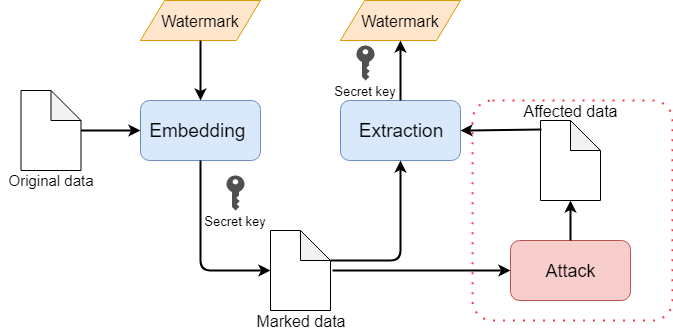
\includegraphics[width=\textwidth]{Figures/framework.png}
    \caption{General framework for watermarking}
\end{figure}

\section{Watermark categorisation}

Digital watermarks may be categorised in several ways depending on different properties. 
The following categorisation criteria are applied to fingerprints as well since we consider fingerprinting as a special case of watermarking. 

\paragraph{Imperceptibility}
The most general categorisation is according to the imperceptibility of a watermark. A digital watermark is called \textit{imperceptible} if the marked copy is perceptually indistinguishable from the original data. 
A watermark is \textit{perceptible} if its presence in the data is noticeable (e.g. owner's logo as an overlay on an image).

\paragraph{Detectability}
Watermark schemes can be categorised in terms of verifiability / detectability, i.e. needing the original data to extract the watermark from the marked data. A \textit{Blind} watermarking scheme does not need the original data for the extraction process, while \textit{non-blind} does. 

\paragraph{Robustness}
Furthermore, according to its robustness, watermarks can be categorised into \textit{fragile}, \textit{semi-fragile} and \textit{robust}.  
Fragile watermarks are commonly used for tamper detection because they fail to be detected after the slightest modification. 
Semi-fragile transformation resists some benign transformations, but fail detection after malignant transformations (attacks). 
Robust watermarks resist a wide range of benign or malignant transformations and satisfy the property that the removal of a watermark is not possible without significantly degenerating the data quality.

\paragraph{Distortion}
In \textit{distortion-based} watermarking techniques marking introduces distortions to the underlying original data. 
On the contrary, \textit{distortion-free} watermarking techniques rely on detecting the watermark as a function of the data itself without changing the original data. 
Distortion-free watermarks are fragile and are applied in tamper detection.

\section{Multimedia, text and software}
The concepts of watermarking \cite{cox1997secure, petitcolas2000information, lee2001survey} and fingerprinting \cite{wu2004collusion} digital data firstly appear in domains of multimedia data and are extensively studied over the last two decades.
Most of these techniques are developed for images \cite{o1996watermarking} and later extended to video \cite{hartung1998watermarking} and audio \cite{boney1996digital,swanson1998robust}.

Image watermarking is applied in two main domains of an image: in the spatial domain where an image is represented by pixels and in the transform domain where it is represented in terms of its frequencies (the image is segmented into multiple frequency bands using a mathematical transform, for instance, Discrete Cosine Transform (DCT), Discrete Wavelet Transform (DWT) and Discrete Fourier Transform (DFT)) \cite{potdar2005survey}.
The watermark can be embedded in the spatial domain by modifying pixel values \cite{nikolaidis1998robust} or adding an overlying layer on top of the original image \cite{piec2014real}, however more robust watermarks are usually embedded in the transform domain by modifying the transform domain
coefficients \cite{suhail2003digital,solachidis2001circularly}.
More advanced watermarking techniques are developed for video watermarking which extends and incorporates watermarking techniques for images \cite{wolfgang1999perceptual,swanson1998multiresolution}. 
Most of the image and video watermarking algorithms focus on processing data files stored on a disc, while some introduce real-time content processing (applied for example on screenshot images) \cite{piec2014real,kang2006implementation}.

There have also been some approaches in applying a watermarking scheme in other domains such as text and software. 
Techniques for watermarking text data typically exploit
special properties of text formatting and semantics. 
Watermarks are often introduced by altering the spacing
between words and lines of text \cite{maxemchuk1994electronic}. 
Other techniques rely on natural language processing and rephrasing sentences in the text \cite{atallah2001natural, atallah2000natural, atallah1999watermarking, atallah2002natural}.
Techniques for watermarking software only have limited success in their native domain \cite{palsberg2000experience,collberg1999software}.
A key problem is that the instructions in a computer program can often be rearranged without altering the semantics of the program. This resequencing can destroy a watermark. 
Techniques have also been proposed to prevent copying of software, but they require installation of tamper-resistant modules in users’ machines, which limits their successful adoption in practice.

\section{Watermarking Relational Databases}
Digital watermarks in the domain of multimedia are not easily extended or adapted to relational database applications, because of the inherent differences between multimedia data and relational databases.
For example, a lot of techniques for images and audio rely on phenomena based on the limitation of the human visual and auditory system. Furthermore, multimedia data contains a large number of redundant bits providing much wider cover for embedding the watermark than it is the case with relational data. 
Relational data may as well consist of multiple types of data - numerical, categorical, text, etc., requiring different approaches for embedding the watermark. 
Categorical data is known to introduce additional issues for watermarking compared to numerical, so we will divide these techniques into separate subsections.
Therefore, techniques for watermarking relational data differ significantly from those for multimedia. 
A couple of surveys \cite{rathva2013watermarking,mehta2014watermarking,iftikhar2015survey,kamran2018comprehensive} list most of the proposed watermarking techniques in the literature and classify them, comparing thereat their main properties and robustness to attacks. 
In the remainder of the section, we present the watermarking techniques for relational data, according to the categorisation illustrated in \Cref{fig:categorization} \cite{halder2010watermarking}. 
The first level of categorisation is a distinction of watermarks based on distortion. Distortion-based watermarks are then divided into categories based on the type of data they apply to. A further distinction is made among the techniques applied to a numerical type of data according to what carries the watermark information. 

\begin{figure}
    \centering
    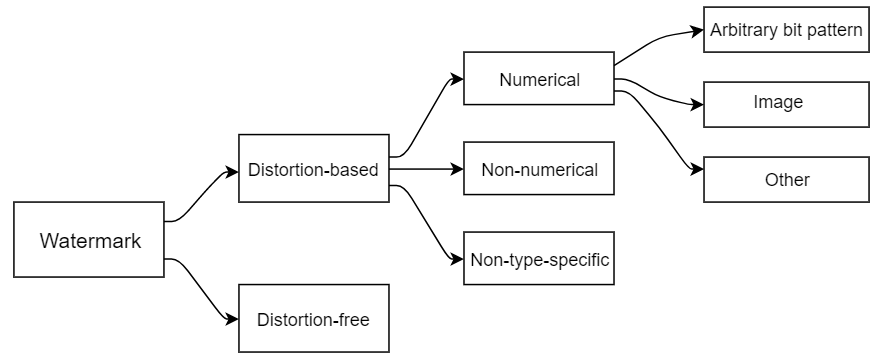
\includegraphics[width=\textwidth]{Figures/categorization.PNG}
    \caption{Categorization of watermarking techniques for relational data}
    \label{fig:categorization}
\end{figure}

\subsection{Distortion-based watermarks}
\subsubsection{Watermarking numerical data}
\begin{enumerate}[leftmargin=*]
    \item \textit{Arbitrary bit pattern as watermark information}
\paragraph{}
Pioneering work on watermarking relational databases is proposed by Agrawal and Kiernan \cite{agrawal2002watermarking}. It is a blind, bit-resetting technique where the watermark insertion is controlled by a gap parameter $\gamma$ (the ratio of tuples to be fingerprinted). 
They use a message authentication code (MAC) - a one-way hash function that depends on a secret key to determine which tuples will be marked. 
The same value $\mathcal{F}(r.P)=\mathcal{H}(\mathcal{K}||\mathcal{H}(\mathcal{K}||r.P))$ is used for selecting the tuple, attribute and bit that will be marked, where $\mathcal{H}$ is a hash-function, $\mathcal{K}$ is a secret key, $r.P$ the primary key of the tuple and $||$ is representing a concatenation.
The important property of a hash function is that it is easy to calculate a hash value (output) for a given input, but computationally difficult to do the reverse. 
Therefore only the owner knowing the secret key can detect where the marks are embedded in the data.
\paragraph{}
This work is extended in \cite{agrawal2003system, agrawal2003watermarking} by introducing a pseudo-random sequence generator instead of the MAC in the process to select tuples, attributes and bits for watermarking.
The technique from \cite{agrawal2003watermarking} (referred to as the AKH technique; AKH stands for the initials of the authors) and its predecessor \cite{agrawal2002watermarking} is used for many extended works in watermarking and fingerprinting relational databases.
The technique in principle contains two steps: watermark insertion and watermark detection, according to the generic framework for watermarking. 

The \textit{watermark insertion algorithm} marks certain numerical attributes such that the least significant bits (LSBs) are altered, therefore this technique assumes that the dataset contains one or more numerical attributes.
The database owner is left to decide the number of LSBs available for marking $\xi$, such that the changes of marked attributes stay imperceptible. 
The insertion algorithm then uses a cryptographic pseudo-random sequence generator $\mathcal{G}$, seeded by a secret key known only to the owner of the database, and concatenated with the primary key attribute value of each tuple from a database. 
The main assumption that the AKH technique relies on is the existence of a primary key in the dataset. 
Li et. al. \cite{li2003constructing} propose three different schemes to obtain a virtual primary key for relational databases without primary key.
The numbers generated by $\mathcal{G}$ determine the tuples, attributes within the tuples and LSBs within the attribute values to be marked, as well as the mark itself. 
It is computationally infeasible to predict the next number in the cryptographic pseudo-random sequence.
Thus, it is computationally infeasible to guess the marking pattern without the knowledge of the owner’s private key. 

The \textit{detection algorithm} contains calculating the sequence using a cryptographic pseudo-random sequence generator with the same seeds as in the insertion algorithm. 
Those sequences will be the same because repeated executions of the generator seeded by the same value always produce the same sequence. 
Thus, the detection algorithm finds which bits within the database should have been marked and counts how many of them match the bits from the database suspected for piracy. 
If the number of matches is “large”, the database owner can suspect the piracy. 
On the other hand, if the matching is “too small”, the database owner can suspect that the attacker somehow identified the marking pattern and recreated the original database values.
The number of matches necessary for suspecting piracy is defined by a parameter $\tau$ called \textit{significance level}. 

The authors analysed the robustness of this technique against several malicious attacks, namely, subset attacks, bit-flipping attacks, mix-and-match attack and false claim of ownership. 
More of the robustness analysis of the AKH scheme is done in later work by Lafaye \cite{lafaye2007analysis}.
\paragraph{}
Extensions and improvements to the AKH technique have been proposed in \cite{qin2006watermark} and \cite{gupta2009database}. 
The first one \cite{qin2006watermark} improves the AKH by using chaotic random series based on the Logistic chaos equation instead of a hash function. 
This has two advantages: non-repetitive iterative operation and sensitiveness to initial values in a way that the selection of bits meets the requirements of both data range and data precision of each attribute, rather than using same $\xi$ for all attributes as it is the case in the AKH. 
This strategy's advantages manifest by a significantly decreased error when data with large differences in ranges within the attributes is watermarked. 
Another extension is a reversible version of the AKH watermarking scheme \cite{gupta2009database} where watermark can be recovered during the detection phase and the attribute can be restored to its unmarked value.

The watermarking method in \cite{xiao2007second} embeds random digits at second LSB positions of the numeric candidate attributes. The watermark is not explicitly embedded like in the previously mentioned techniques, but rather used for identifying valued groups of tuples to embed the random values.

\item \textit{Image as watermark information}

There is a couple of proposed techniques that mark the data using an image as watermark information.
\paragraph{}
The method in \cite{wang2008atbam} describes embedding the scrambled image based on the Arnold transform with scrambling number \textit{d}. 
The scrambling number improves the security of this technique because of it an additional parameter, besides the secret key, that the embedding scheme relies on.
The scrambled image is represented as a binary string and embedded into tuples that are previously grouped using hash values depending on a secret key, primary key and the order of the image. 

Another method \cite{hu2009image} follows the similar algorithmic steps as in \cite{wang2008atbam}, but embeds the original image converted into a bit flow instead of a scrambled image.

The method in \cite{zhou2007additive} divides an image into \textit{header} and \textit{image data}  in the insertion phase. The header is used in a hash function together with tuple's primary key to determine tuple's ID value and determine positions where the image data will be embedded.

\item \textit{Other types of watermark information}

Besides arbitrary meaningless bit pattern and image as watermark information, other types of watermark information have been proposed and embedded into the data.
One example is speech as a watermark information \cite{wang2008speech}. The proposed technique uses compressed owner's speech converted into a bitstream as a watermark and follows similar algorithmic steps as \cite{hu2009image}.
Furthermore, in \cite{cui2008approach} authors propose a Genetic Algorithm-based technique to generate watermark signal, in \cite{zhang2005method} the cloud watermarking scheme is proposed and authors in \cite{huang2009cluster} use \textit{k-means} algorithm to cluster the tuples into some equivalent classes.

Watermark information may as well be the content of data itself \cite{zhang2006relational, guo2006fragile}.
Generally, some bits of one part of the data, i.e. characteristics are extracted in the insertion phase and used to mark the other parts of the data. 
\end{enumerate}

\subsubsection{Watermarking non-numerical data}
Non-numerical data requires different techniques for watermarking purposes than numerical data because of its discrete nature. 
The concept of introduced errors is perceived differently as well because we cannot apply the same measurements as in the case of categorical data, e.g. marking the numerical value 23 as 25 does not have the same impact on the data as marking "blue" as "red". 
The latter may not even be acceptable in some settings, therefore watermarking non-numerical data needs to start from the assumption that the user accepts this kind of errors and that they do not violate credibility and utility of the data. 
Another limitation of watermarking categorical data that can cause the loss of credibility is the semantic correlation between the attributes that depending on the setting needs to be preserved.

In \cite{sion2004proving,sion2005rights} the authors propose a technique for watermarking categorical data.
The technique requires the presence of a primary key in the dataset.
The embedding process relies on two secret keys $k_1$ and $k_2$.
The first secret key $k_1$ is used for selecting the tuples "fit" for watermarking together with parameter $e$ and the primary key. 
$e$ is a control parameter of how many tuples get marked, i.e. has the same purpose as parameter $\gamma$ in schemes for watermarking numerical data. 
The number of tuples "fit" to be marked ($\eta/e$) is usually larger than the size of a watermark, which is solved by converting the watermark $wm$ into $wm\_data$ of length $\eta/e$ using an Error Correcting Code (ECC). 
In every "fit" tuple, the embedding algorithm generates a secret value in bit representation. 
The number of bits in a secret value is equal to the number of bits required to represent all possible categorical values for the attribute. 
The least significant bit of the value is marked by a randomly chosen bit of $wm\_data$ depending on the primary key and the secret key $k_2$. 
The marking scheme assures that the resulting categorical value will be some value from the domain of the attribute.
The pseudo-random nature of the choice of a bit from $wm\_data$ guaranties that almost all bits will be chosen at least once during the embedding process. 
Using two different secret keys $k_1$ and $k_2$ assures non-correlation between the selected tuples for embedding and the corresponding bit value positions in $wm\_data$. 

The detection algorithm reverses the operations from the insertion phase and extracts some $wm\_{data}'$. Once $wm\_{data}'$ is available, the ECC is invoked to generate the "closest" or "most likely" corresponding watermark $wm$. 

The authors also suggest an embedding scheme based on multiple categorical attributes by considering not only the association between the primary key and a single categorical attribute but also associations between different categorical attributes. 
The embedding scheme described previously is applied for every combination of \textit{primary key - categorical attribute}, and every combination of two categorical attributes. In combinations of two categorical attributes, one of them serves as a virtual primary key for the embedding process. 
For instance, let us have a dataset containing primary key \textit{K} and two categorical attributes $C_1$ and $C_2$. 
The embedding scheme will be performed 3 times, for $(K,C_1)$, $(K,C_2)$ and $(C_1,C_2)$. 
First, two runs of the embedding scheme will use the secret key $k_1$, $e$ and the primary key $K$ for the choice of tuples to be marked and embeds the mark in attribute $C_1$ (or $C_2$ for the second combination).
The embedding scheme run for $(C_1,C_2)$ uses the secret key $k_1$, $e$ and attribute $C_1$ for the choice of tuples to be marked and embed the mark in attribute $C_2$.
In this scheme for watermarking multiple categorical attributes, taking just described case, we can see that markings for $(K,C_2)$ interfere with markings for $(C_1,C_2)$. 
Even though this scheme is claimed to be robust against serious attacks (e.g. vertical data partitions) and breaks the dependency of the primary key, the convenience of this method is questionable due to the increase of the number of combinations (sequence of triangular numbers) for more categorical attributes in the dataset.

This watermarking technique is applied to binned medical data in \cite{bertino2005privacy}.

Another method for watermarking non-numerical data has been proposed in \cite{al2008robust}, for non-numeric multi-word attributes. The watermarking scheme is based on hiding a binary image in space of non-numeric multi-word attributes of subsets of tuples by introducing double spaces on pseudo-randomly chosen places. The scheme is claimed to be robust against subset and superset attacks, however, it may suffer from the simple malicious action that replaces all double spaces between two words by a single space and therefore erases the watermark.  

\subsubsection{Watermarking non-type-specific data}
Techniques have been proposed to use fake tuples \cite{pournaghshband2008new} or fake attributes \cite{prasannakumari2009robust} as watermark information. 

The approach from \cite{pournaghshband2008new} generates fake tuples and inserts them erroneously into the dataset. 
The fake tuple creation algorithm uses Bernoulli sampling probability to decide whether the new value will be chosen from the existing set of values of the corresponding attribute, or a set of fake values. 
The choice of the new value can be made uniformly, or as the value with higher-occurrence frequency in the existing set of values of the corresponding attribute in the relation. 
The detection algorithm checks via the primary key to see whether the fake tuples inserted during watermarking insertion phase exist or has been changed. As soon as it finds one match, detection is done. 
The detection fails for the watermarked database when all of the fake tuples are deleted.
One advantage of this scheme is that the owner can be publicly verified more than once until all of the fake tuples are revealed.
Another advantage is that this scheme works with all types of values - numerical, categorical, dates, etc.

The technique of inserting a virtual attribute in the relation which serves as watermark \cite{prasannakumari2009robust} generates new values as aggregates obtained from any other numerical value from the dataset. 
This approach is fragile and can easily detect any of the deletion, insertion or alteration attacks, however, it suffers from the watermark removal attack.  

\subsection{Distortion-free Watermarking}
The watermark information may be the hash value extracted from the data.      
The main idea is to partition the data in some way. 
\cite{li2004tamper} propose a technique where partitioning of tuples is based on the hash value parameterized with the primary key and secret key, whereas in \cite{bhattacharya2010distortion}, partitioning is based on categorical attribute values. 
After partitioning, hash values for each group as well as tuple level hash values are computed. Based on the hash values and their parity, two tuples' order changes or doesn't. 
These schemes are able to detect any modifications made to a database relation.

There are other proposed solutions in the literature that are used as watermark information, such as combining owner's mark and database features \cite{tsai2006database}, converting database relation into binary form \cite{li2006publicly,bhattacharya2009generic} or R-tree based permutations \cite{kamel2009schema}.

Most of the distortion-free watermarking techniques are fragile, i.e. they aim at maintaining the integrity of the information in the database in addition to the ownership protection. 
The watermark insertion phase does not depend on any specific type of data and does not introduce any distortion in the underlying data of the database.

\section{Fingerprinting Relational Databases}

Fingerprinting is a special application of watermarking - a distinct watermark (a fingerprint) is generated and embedded in every distributed copy of the data. 
In paper \cite{kamran2018comprehensive}, the authors gave a classification and brief analysis of relevant watermarking and fingerprinting techniques. \Cref{tab:comparison_fingerprinting} is derived from this survey. 
In our review we mention many of the techniques from \cite{kamran2018comprehensive} and include some that are not mentioned in the survey.

Li et al. in \cite{li2005fingerprinting} extended the watermarking technique proposed by Agrawal et al. \cite{agrawal2003watermarking} into a fingerprinting technique.
The marking scheme embeds different bit-strings - \textit{fingerprints} in different releases of data.
The owner generates buyer’s fingerprint from the owner’s secret key and the buyer’s serial number using a cryptographic hash function.
This method of generating the fingerprints avoids storing buyer-fingerprint pairs and additional security management for this database.
Similarly to the watermarking technique \cite{agrawal2003watermarking}, this fingerprinting technique consists of the insertion algorithm and detection algorithm. 

The insertion algorithm follows the steps for selecting the tuple, attribute, LSBs and marks in the same manner as the insertion scheme from \cite{agrawal2003watermarking}, and additionally embeds the generated fingerprint by XOR function applied on the mark (in this algorithm called \textit{mask}) and a selected fingerprint bit. 

The aim of the detection algorithm of the fingerprinting methods, in general, is to determine whether the suspicious database is pirated, as well as to identify the source of the unauthorised release of the database. 
The detection algorithm from \cite{li2005fingerprinting} reverts the fingerprint insertion process similarly to \cite{agrawal2003watermarking}. It locates the bits that should have been altered and compares the matching of the extracted fingerprint with buyers’ fingerprints. 
The exact bit matching of the extracted fingerprint to some buyer’s fingerprint implies this buyer to be an unauthorised distributor.
$\tau$ is a parameter related to the assurance of the detection process.
\paragraph{}
In \cite{liu2004block}, authors propose a block-oriented fingerprinting scheme for relational databases inspired by a fingerprinting scheme for images from \cite{das2002robust}. 
This method also relies on altering the LSBs at certain locations in the database. 

In the insertion algorithm, the LSBs of numerical values from the database (as much LSBs as it is allowed to change) are combined into a two-dimension image and separated into blocks of size $\beta\times\beta$. 
Then a pseudo-random number generator is used to decide the block and position within the block where the fingerprint should be embedded until all blocks are marked. 
Fingerprint bits will be embedded again if there is still unmarked blocks left when all fingerprint bits have been embedded. 
A fingerprint is produced in the same manner as in previous techniques, using the cryptographic hash function seeded by the owner’s secret key and the user’s serial number.

Detection phase consists of sorting the suspicious database according to the primary keys and filling out the database with the original values in case of deletion. 
The location where the fingerprint bit is supposed to be is calculated as in insertion algorithm and the bit is recorded. 
As the fingerprint is embedded multiple times in the dataset, if most of the detected values for a single fingerprint bit are 1, the detected fingerprint is said to be 1, otherwise 0. 
\paragraph{}
Authors of watermarking and fingerprinting system \textit{Watermill} \cite{constantin2005watermill, lafaye2008watermill} further extend the methods from \cite{agrawal2003watermarking} and \cite{li2005fingerprinting} by considering the constraints of data alteration and treating fingerprinting as an optimisation problem. 
By using a declarative language, the usability constraints that the fingerprinted dataset must meet are specified. For example, a purchaser may require that joins between some attributes should be preserved, or that values of some attribute cannot be altered more than a predefined amount. 
One of two proposed fingerprinting strategies consists of translating the weight-independent constraints into an integer linear program (ILP) and using the ILP solver to solve it. 
The second fingerprinting strategy is \textit{pairing heuristics} for larger datasets where using ILP solver might not be efficient.

\paragraph{}
In \cite{guo2006fingerprinting} and in its predecessor \cite{guo2005improved}, the proposed technique is a two-level fingerprinting scheme. 
In the first embedding process, a distinct fingerprint of length $L$ for each buyer is embedded. The tuples are partitioned into $L$ subsets and in each of them, one fingerprint bit is embedded in a pseudo-random position. 
The second embedding process is designed for verifying the extracted fingerprint and numerical confidence level. 
The selected positions are marked as "0" or "1" depending on the hash value seeded with secret key concatenated with the primary key.
A fingerprint from the first level is used as a secret key for the second embedding level.
To avoid conflict between two levels of embedding, the bit values in the second embedding process are only considered for marking if not marked in the first embedding process.
\paragraph{}
In \cite{zhou2007novel} an architecture for identifying a malicious buyer and redistributing digital content is proposed. 
When a user accesses the database, a fingerprinting process is invoked. 
A parameter manager module is used to store the fingerprinting parameters and a manager module is in charge for the fingerprinting task and verifying authenticity of users; if the user is unauthentic (not the owner), the fingerprinting process is executed. 
The encoding and decoding algorithm is the same as in \cite{guo2005improved}.
\paragraph{}
All of the above fingerprinting techniques have one restriction in common - they are applicable only on numerical attributes. Only a few solutions have been proposed for the categorical data.

One approach is a fingerprinting technique that incorporates the k-anonymity property into the fingerprinted data \cite{Kieseberg2014fingerprinting}.
k-anonymity~\cite{Sweeney2002} strives to modify a dataset so that at least \textit{k} data samples (individuals) become indiscernible when considering quasi-identifying attributes. This is commonly achieved by generalising values in the dataset to a broader meaning. There are generally multiple solutions for achieving the same level of \textit{k} by choosing different attributes to modify.
The idea of the scheme is, therefore, that equivalent k-anonymous patterns of the given dataset serve as fingerprints, and the process of anonymizing data is at the same time the fingerprinting process.
K-anonymity is applied on both categorical data and numerical, therefore this model, unlike the previous, provides the fingerprinting technique that includes the categorical data in the process.
However, there are some limitations: (i) the number of available fingerprints is limited to the number of different equivalent patterns for k-anonymity in the dataset, (ii)  the utility of the differently fingerprinted (anonymized) datasets can vary significantly, and (iii) the fingerprint cannot be computed alone by the recipient's identifier, but rather, a mapping of fingerprint and recipients needs to be stored, with all associated security risks.

\begin{table}[ht]
    \centering
    \caption{Summary and comparison of well known fingerprinting techniques}
    \label{tab:comparison_fingerprinting}
    \resizebox{\textwidth}{!}{
    \begin{tabular}{|c|c|c|c|c|c|c|c|}
    \hline
         Scheme & \begin{tabular}{c}
              \\ Attribute \\data type 
         \end{tabular} & \begin{tabular}{c}
              Attribute \\ selection \\ method
         \end{tabular} & \begin{tabular}{c}
              Tuple \\selection \\ method
         \end{tabular} & \begin{tabular}{c}
              \\ Granularity \\ level  
         \end{tabular} & \begin{tabular}{c}
              \\ \\ Detectability  
         \end{tabular} & \begin{tabular}{c}
              \\ \\ Dependencies  
         \end{tabular} \\
         \hline\hline
         AK \cite{li2005fingerprinting} & Numerical & PRSG & PRSG & Bit & Blind & \begin{tabular}{c}
              Primary key, \\ Value
         \end{tabular} \\
         \hline
         Block Scheme  \cite{liu2004block} & Numerical & All & All & Bit & Not Blind & \begin{tabular}{c}
              Primary key, \\ Value
         \end{tabular} \\
         \hline
         Watermill \cite{lafaye2008watermill} & Numerical & Arbitrary & PRSG & Bit & Blind & \begin{tabular}{c}
              Primary key, \\ Value
         \end{tabular} \\
         \hline
         \begin{tabular}{c}
              Two-level \\ scheme \cite{guo2006fingerprinting} 
         \end{tabular} & Numerical & Arbitrary & SHF & Bit & Blind & \begin{tabular}{c}
              Primary key, \\ Value
         \end{tabular} \\
         \hline
         FP Architecture \cite{zhou2007novel} & Numerical & Arbitrary & SHF & Bit & Blind & \begin{tabular}{c}
              Primary key, \\ Value
         \end{tabular} \\
         \hline
         \begin{tabular}{c}
              k-anonymity \\ based \cite{Kieseberg2014fingerprinting} 
         \end{tabular} & All & All & All & Value & Blind & Value \\
         \hline
    \end{tabular}}
\end{table}


\chapter{Fingerprinting techniques}\label{sec:Fingerprinting}
Fingerprinting is a technique that embeds a piece of information into the data to provide the identification of the owner of data and the source of potential unauthorised data leakage. 
Fingerprint combines secret owner-specific and buyer-specific information and is embedded in the dataset. 
Every buyer has her fingerprint, therefore every dataset fingerprinted and distributed by the owner is different from each other.
By detecting the fingerprint within the dataset, the owner can trace the buyer of that instance of the dataset. 
The fingerprinting techniques usually contain two main algorithms: fingerprint insertion and fingerprint detection. 
In the fingerprint insertion, the fingerprint of a buyer is embedded into the dataset.
Fingerprint detection strives for detecting the fingerprint in a suspicious dataset to connect it with the buyer who distributed the dataset without the authorisation.
Detection could be disrupted by malicious attempts of the buyer to remove the fingerprint from the data, but also by benign changes in the dataset. 
These attacks and fingerprint resistance to them will be addressed in \Cref{sec:Robustness}.


\section{Notation and parameters}
In the following, several different fingerprinting techniques are discussed in detail. 
In this section, we set the common notation and explain the parameters used in the techniques. 
The dataset schema is denoted by $\mathcal{R}(P,A_0,...,A_{v-1})$ where $\mathcal{R}$ is a database relation, \textit{P} is the primary key attribute, and $A_0,...,A_{v-1}$ are $v$ attributes that will be used for fingerprinting. 
$\eta$ is a notion of number of tuples (rows/entries) in the dataset. 
As the fingerprinting techniques embed the fingerprint by changing the attribute values, we define the parameter $\xi$ which denotes the number of least significant bits (LSBs) that can be used to embed the fingerprint. \\
Let \textit{N} be the number of buyers to whom the dataset is being distributed. 
To each of the buyers, a unique fingerprint will be assigned. 
Every fingerprint $\Gamma = (f_0,...,f_{L-1})$ is a binary string of length $L \geq logN$. \\
Besides the buyer's fingerprint, the owner-specific information has to be embedded in the dataset to ensure the ownership protection and make it possible only for the data owner to detect the fingerprint from the fingerprinted dataset. 
This information is usually a secret key $\mathcal{K}$ - a binary string known only to the dataset owner.
\Cref{table:notation} contains the notation that will be used in the remainder of this thesis unless otherwise stated.

\begin{table}
\centering
\caption{The notions of the most common parameters}
\label{table:notation}
\begin{tabular}{|c | c|} 
 \hline
 Notation & Meaning \\ 
 \hline\hline
 $\mathcal{R}$ & database relation \\
 \hline
 \textit{P} & primary key attribute \\
 \hline
 $A_i$ & attribute $i$ \\
 \hline
 \textit{v} & number of attributes \\
 \hline
 $\eta$ & number of tuples  \\
 \hline
 $\mathcal{K}$ & owner's secret key  \\
 \hline
 $\xi$ & number of least significant bits \\ 
 \hline
 $1/\gamma$ & ratio of tuples to be marked\\
 \hline
 \textit{N} & number of buyers \\
 \hline
 \textit{L} & length of fingerprint \\
 \hline
 $\omega_i$ & number of embeddings of a fingerprint bit $i$ \\
 \hline
 $\omega$ & total number of marks \\
 \hline
\end{tabular}
\end{table}

\section{Prerequisites}
Before discussing the specific schemes and algorithms used for fingerprinting relational databases, it is necessary to mention auxiliary functions and algorithms required to achieve the goal of robust fingerprints. 
Cryptographic pseudo-random sequence generator and cryptographic hash function, discussed in the following subsections, both ensure that neither the fingerprint nor any part of fingerprinting scheme get disclosed or recreated by an unauthorised user.
This stated, their usage is crucial for the owner's rights protection.

\subsection{Cryptographic pseudo-random sequence generator}
A cryptographically secure pseudorandom number generator (CSPRNG) is an algorithm for creating a sequence of random numbers with properties suitable for use in cryptography.
The CSPRNG-generated sequence is not truly random, because it is completely determined by the initial value called \textit{seed}. 
The requirements of CSPRNG fall into two groups: 
\begin{itemize}
    \item They pass statistical randomness tests. 
    
    A generator passing the \textit{next-bit test} will pass all other polynomial-time statistical tests for randomness (proof by Andrew Yao in 1982 \cite{yao1982theory}). We say that a sequence of bits passes the next-bit test for at any position $i$ in the sequence, if any attacker who knows the $i$ first bits (but not the seed) cannot predict the $(i+1)$st with reasonable computational power.
    
    \item They resist a serious attack, even when part of their initial or running state becomes available to an attacker.
    
    If part or all of CSPRNG's state has been revealed (or guessed correctly), it should be impossible to reconstruct the stream of random numbers before the revelation. Additionally, if there is an entropy input while running, it should be unfeasible to use knowledge of the input's state to predict future conditions of the CSPRNG state.
\end{itemize}

There is several designed practical CSPRNGs including the Yarrow Algorithm \cite{kelsey1999yarrow} incorporated in iOS and macOS, its successor Fortuna \cite{ferguson2015generating} used in FreeBSD, CryptGenRandom \cite{cryptgenrandom} included in Microsoft's Cryptographic Application Programming Interface, etc.

For the analysis in the thesis, we denote CSPRNG with $\mathcal{S}$, where $\mathcal{S}_i$ denotes the $i^{th}$ random number of the sequence.

\subsection{Cryptographic hash function}
The cryptographic hash function is a deterministic function that takes a string input of any length and returns a fixed-size string value. 
The returned value is called "hash value". 
In literature the hash value can be also referred to as "digest", "checksum" or "digital fingerprint" (the word \textit{fingerprint} is here used in the different context than the \textit{fingerprint} used as a topic of this thesis).
The hash function has three main properties:
\begin{itemize}
    \item It is easy to calculate a hash value for any given input string.
    \item It is computationally difficult to calculate an input that has given a certain hash value.
    \item It is extremely unlikely that two different inputs, even remotely different, have the same hash value.
\end{itemize}

While the regular hash functions aim to, most importantly, avoid the collision of hash values for non-malicious input, the above properties are much strongly guaranteed for cryptographic hash functions.  
The hash value serves as a "signature" for the input provided.
Only the person knowing the original input value can easily check the matching hash function. 
However, knowing only the hash value, one is unable to do the inverse and find out the original input value. 
If either finding a string that matches a given hash value or finding two different inputs that have the same hash value is computationally feasible, then a cryptographic function is not considered secure from a cryptographic point of view.

Most commonly used cryptographic hash functions are MD5 \cite{rivest1992md5} and SHA-1 \cite{eastlake2001us}.


\section{Fingerprint codes}
A fingerprinting scheme assigns a specific fingerprint to each of the \textit{N} buyers.
A fingerprint is a unique binary string of length \textit{L} known only by the database owner which is used to trace a specific owner. 
Storing the mapping of a recipient to her fingerprint is additional data that requires additional protection measures to be protected against attacks.  
To avoid this, the owner uses a cryptographic hash function $\mathcal{H}$ to produce each buyer's fingerprint instead.
In the fingerprinting techniques presented in the following sections, each fingerprint $\mathcal{F}$ is produced as a hash value of the concatenation of owner's secret key $\mathcal{K}$ and buyer's identification number \textit{id}:
\begin{equation}
    \mathcal{F}(\mathcal{K},id)=(f_0,...,f_{L-1})=\mathcal{H}(\mathcal{K}|id)
\end{equation}
where buyer's identification number can be publicly accessible.
This way only the owner who knows both secret key $\mathcal{K}$ and identification number \textit{id} can produce the hash value - the fingerprint of a specific buyer.

\paragraph{Collusion resistant codes}
Fingerprinting schemes are susceptible to collusion attacks where users with multiple copies of the same dataset but different embedded fingerprints work in coalition to create a useful data copy that does not implicate any member of the coalition. 
Collusion attacks will be thoroughly discussed in \Cref{subsec:collusion}, while in this section we cover collusion resistant codes.
Collusion resistant fingerprinting codes have been studied extensively in the literature \cite{boneh1998collusion, guth1999error, pfitzmann1999coin, pfitzmann1996asymmetric, yacobi2001improved}. 
One of the well-known codes is proposed by Boneh and Shaw \cite{boneh1998collusion} (this code is referred to as \textit{BoSh code} in the remainder of the thesis). 
The effectiveness of the BoSh code relies on the assumption that colluding buyers can detect only the fingerprint bits in which their copies differ, otherwise a fingerprint bit cannot be detected.
For example, two buyers with their own fingerprinted datasets can easily compare their datasets and remove or change the values that differ between their copies. 
Authors of \cite{boneh1998collusion} call refer to this as the "Marking Assumption". 
The main property that codes should satisfy is that users cannot change the state of an undetected bit without rendering the dataset useless. 
This small amount of information where the buyers' marks agree is used to trace the copies they generate back to either of them.
A collusion resistant code is expected to have two properties well-elaborated:
\begin{itemize}
    \item $c$-frameproof code, i.e. a coalition of at most $c$ users cannot frame a user not in the coalition even all user fingerprints are known to the users
    \item $c$-secure code, i.e. there exists a tracing algorithm that on input $x$ must output a single member of the coalition of at most $c$ users, where the input $x$ is the new mark extracted by the fingerprint extraction algorithm that was generated by the coalition
\end{itemize}
The usage of the BoSh code is discussed in \Cref{subsec:ak} as a part of the collusion-resistant version of the scheme. 

\section{AK Scheme}\label{subsec:ak}

\begin{algorithm}
  \KwIn{dataset $\mathcal{R}$ with scheme $(P, A_{0}, ..., A_{v-1})$, buyer $n$'s ID $id$}
  \KwOut{fingerprinted dataset $\mathcal{R'}$}
  fingerprint of buyer $n$: $\mathcal{F}(\mathcal{K},id)=\mathcal{H}(\mathcal{K}|id)$
  \\
  \ForEach{tuple $r \in \mathcal{R}$}
  {
    \If{$(\mathcal{S}_{1}(\mathcal{K}|r.P)$ mod $\gamma == 0)$}{
        attribute\_index $i = \mathcal{S}_2(\mathcal{K}|r.P)$ mod $v$
        \\
        bit\_index $j=\mathcal{S}_3(\mathcal{K}|r.P)$ mod $\xi$
        \\
        mask\_bit $x=0$ if $\mathcal{S}_4(\mathcal{K}|r.P)$ is even; $x=1$ otherwise
        \\
        fingerprint\_index $l=\mathcal{S}_5(\mathcal{K}|r.P)$ mod $L$
        \\
        fingerprint\_bit $f=f_l$
        \\
        mark\_bit $m=x \oplus f$
        \\
        $LSB(j,r.A_i) = m$
    }
  }
  \Return{$\mathcal{R'}$}
  \caption{AK Scheme: Insertion Algorithm}
  \label{alg:AK-insertion} 
\end{algorithm}

\begin{algorithm}
  \KwIn{fingerprinted dataset $\mathcal{R'}$ with scheme $(P, A_0, ..., A_{v-1})$}
  \KwOut{suspected buyer's ID $id$}
  //initiate fingerprint template and counts \\
  fingerprint template $\mathcal{F}=(f_0,...,f_{L-1})=(?,...,?)$ // '?' represents unknown value \\
  \For{$i=0$ to $L-1$}
  {
    $count[i][0]=count[i][1]=0$ \\
    // $count[i][0]=count[i][1]$ are votes for $f_i$ to be 0 and 1 respectively
  }
  //scan all tuples and obtain counts for each fingerprint bit \\
  \ForEach{tuple $r \in R'$}
  {
    \If{$\mathcal{S}_1(\mathcal{K},r.P)$ mod $\gamma==0$}
    {
        attribute\_index $i=\mathcal{S}_2(\mathcal{K},r.P)$ mod $v$\\
        bit\_index $j=\mathcal{S}_3(\mathcal{K}, r.P)$ mod $v$\\
        mark\_bit $m=LSB(j, r.A_i)$\\
        mask\_bit $x=0$ if $\mathcal{S}_4(\mathcal{K},r.P)$ is even; $x=1$ otherwise\\
        fingerprint\_bit $f=m \oplus x$\\
        fingerprint\_index $l=\mathcal{S}_5(\mathcal{K},r.P)$ mod $L$\\
        //update the votes\\
        $count[l][f]++$ 
    }
  }
  //recover the fingerprint\\
  \For{$l=0$ to $L-1$}
  {
    \If{$count[l][0]+count[l][1]==0$}
    {
        \Return{\textit{none suspected}}
    }
    $f_l=0$ if $count[l][0]/(count[l][0]+count[l][1])>\tau$\\
    $f_l=1$ if $count[l][1]/(count[l][0]+count[l][1])>\tau$\\
    \Return{\textit{none suspected}} otherwise
  }
  $\mathcal{F}=(f_0,...,f_{L-1})$\\
  //determine a source of leakage\\
  $id=detect(\mathcal{F,K},L, N)$\\
  \uIf{$id\geq0$}
  {
    \Return{$id$}
  }
  \Else
  {
    \Return{\textit{none suspected}}
  }
  \caption{AK Scheme: Detection Algorithm}
  \label{alg:AK-detection} 
\end{algorithm}

\begin{algorithm}
  \textit{detect}(template $\mathcal{F}$, secret key $\mathcal{K}$, fingerp. length $L$, number of buyers $N$):\\
  \For{each buyer n}
  {
    $\mathcal{F}'=\mathcal{H}(\mathcal{K}|id)$\\
    \If{$\mathcal{F}==\mathcal{F}'$}{\Return{id}}
    \Return{-1}
  }
  \caption{AK Scheme: Subroutine \textit{detect}}
  \label{alg:detect-subroutine} 
\end{algorithm}

In \cite{li2005fingerprinting} the authors describe a fingerprinting scheme that is an extension of the watermarking scheme from \cite{agrawal2003watermarking}. 
In this thesis, this fingerprinting scheme will be referred to as AK Scheme whose name is made of last name initials of authors of the underlying watermarking technique, Rakesh Agrawal and Jerry Kiernan.

\subsection{Algorithms}
\paragraph{Insertion}
Algorithm \ref{alg:AK-insertion} shows the pseudo-code of the insertion algorithm, which is used to embed a fingerprint of a buyer \textit{n} into the dataset $\mathcal{R}$. 
Using random numbers generated by a pseudo-random sequence generator $\mathcal{S}$ the algorithm chooses the bit within the dataset's values that will be marked, as well as the bit that will be embedded.
The pseudo-random sequence generator is independently seeded for each tuple with a concatenation of the owner's secret key $\mathcal{K}$ and the primary key of each tuple. 
In the line 3, the algorithm decides whether the current tuple will be marked, based on the generated number $\mathcal{S}_1(\mathcal{K}, r.P)$. 
In lines 4 and 5, based on $\mathcal{S}_2(\mathcal{K}, r.P)$ and $\mathcal{S}_3(\mathcal{K}, r.P)$, it is decided which one of the attribute's values will be marked, and which least significant bit of the value, respectively. 
In lines 6-10 the algorithm determines which value to replace this bit with. 
The next numbers, generated by the sequence generator $\mathcal{S}_4(\mathcal{K}, r.P)$ and $\mathcal{S}_5(\mathcal{K}, r.P)$, decide the mask bit and choose the fingerprint bit, respectively.
Finally, the resulting bit that is embedded in the line 10 at the chosen place in a dataset is the result of applying XOR function on the mask bit and the fingerprint bit.

\begin{table}[ht]
    \centering
    \caption{Sample dataset}
    \label{tab:exemplary_dataset}
    \begin{tabular}{|c|c|c|}
        \hline
         Primary key & Attribute 0 & Attribute 1  \\
         \hline
         1 & 34 & 749 \\
         \hline
         2 & 21 & 265 \\
         \hline
    \end{tabular}
\end{table}
Assume we want to fingerprint a very simple dataset shown in \Cref{tab:exemplary_dataset} with a fingerprint 11110000.
We use the value 01010101 as a secret key $\mathcal{K}$. 
Furthermore, assume we want to mark on average every second tuple, i.e. $\gamma=2$ and consider the last two bits of value for marking; $\xi=2$.
The algorithm will use the random number sequence generator to produce a unique sequence of numbers for every tuple (different seed for every tuple).
\\Let \\
\hspace*{10 mm} $\mathcal{S}(01010101 | 0) = \{72,39,10,34,97\}$ and \\
\hspace*{10 mm} $\mathcal{S}(01010101 | 1) = \{21,37,62,25,16\}$.

Starting with the first tuple, the algorithm will choose it for marking because $\mathcal{S}_1 \text{ mod } \gamma = 72 \text{ mod } 2 = 0$.
Then the attribute index is chosen as $\mathcal{S}_2 \text{ mod } v = 39 \text{ mod } 2 = 1$ and bit index as $\mathcal{S}_3 \text{ mod } \xi = 10 \text{ mod } 2 = 1$, therefore we are marking 2nd LSB (because bit indices start with 0) of a value 749 which is 0; $751_{10} = 1011101101_2$.
Further, we decide the mark that is going to be applied to the bit. Firstly, the algorithm computes a mask bit as $\mathcal{S}_4 \text{ mod } 2 = 34 \text{ mod } 2 = 0$ and decides which fingerprint bit to use; $\mathcal{S}_5 \text{ mod } L = 97 \text{ mod } 8 = 1$, i.e. second bit of the fingerprint (indices start from 0) - 1.
Secondly, the mark bit value is calculated as $mask\_bit \text{ xor } fingerprint\_bit = 0 \text{ xor } 1 = 1$, and finally the mark bit is embedded into previously chosen place in the data, i.e we are changing 2nd LSB of 749 from 0 to 1 obtaining that way a fingerprinted value 751. 
The algorithm continues with the second tuple. The condition from the line 3 of \Cref{alg:AK-insertion} fails because $\mathcal{S}_1 \text{ mod } \gamma = 21 \text{ mod } 2 = 1$. Thus, the insertion algorithm does not mark this tuple and the process is over. 

\paragraph{Detection}
Algorithm \ref{alg:AK-detection} shows the pseudo-code of fingerprint detection. 
The detection algorithm must reverse the steps from the fingerprint insertion phase to detect all the bits that construct a valid fingerprint. 
In the line 2 of the algorithm, the template for the fingerprint is initialised with \textit{L} unknown values "?".
Reversing the steps from the insertion phase is possible because the pseudo-random sequence generator $\mathcal{S}$ will produce the same random number sequences when seeded with the same value.
Therefore, modelled by the insertion algorithm, it is iteratively seeded with a concatenation of a secret key $\mathcal{K}$ known only to the owner and the primary key of every single tuple.
In lines 9-12, based on random numbers from the sequence, the location of the marked bit is calculated.
In the same manner, the mask bit \textit{x} and fingerprint bit index \textit{i} are calculated, in lines 13 and 15 respectively.
Considering that in the insertion phase the value of a bit to be embedded, i.e. the mark bit \textit{m} is calculated by applying the XOR function on the fingerprint bit and the mask bit, the fingerprint bit \textit{f} is then, in reverse, calculated by applying the XOR function on the mark bit \textit{m} and the mask bit \textit{x} (line 14).
Note that the fingerprinted data set might have been under attack that changes or erases the values from the originally released fingerprinted dataset, for example, subset attack or bit-flipping attack.
This kind of attacks might disturb the fingerprint detection phase and the fingerprint bits might not be detected correctly.
The record of detected values of a fingerprint bit $f_l$ during the detection phase is kept in two count variables $count[l][0]$ and $count[l][1]$ depending if the detected bit is 0 or 1, respectively. 
When the counts for each fingerprint bit are obtained, the algorithm assigns 0 to fingerprint bit $f_l$ if the counts satisfy the condition
\begin{equation}
    count[l][0]/(count[l][0]+count[l][1])>\tau
\end{equation}
or 1 if counts satisfy the condition
\begin{equation}
    count[l][1]/(count[l][0]+count[l][1])>\tau
\end{equation}
The parameter $\tau \in [0.5, 1)$ defines assurance of the detection process.
Recovered fingerprint bits constitute the fingerprint template $\mathcal{F}=(f_0,...,f_{L-1})$ which is compared to fingerprints of buyers to detect the source of leakage. 
This process is done by the subroutine \textit{detect} described in \Cref{alg:detect-subroutine}.
The buyers' fingerprints are calculated on the fly.
If the exact match of buyer \textit{n}'s fingerprint with the fingerprint template is detected, the buyer \textit{n} is reported.

\subsection{Assumptions and Properties}
In this section, we list the assumptions and properties of AK Scheme. 
The first assumption is one that is present in all of the schemes presented in this thesis. 
We have to assume that the minor errors in numerical attributes in the dataset, necessarily caused by fingerprinting process, are not violating the integrity of the database and that those errors are tolerated by the database users. 
Besides, the AK Scheme is modelled such that it requires the presence of a primary key attribute. 
The primary key should stay unmodified or otherwise has to be recoverable for the sake of successful fingerprint detection.
The same is true for the tuple order in the database.
Since each tuple is assumed to have a unique primary key value based on which it is processed independently, the scheme is incrementally updatable. 
This means that fingerprint bits can be added to any additional tuples in the dataset at any given point in time in the future, without breaking the integrity of a fingerprinting scheme.

One more advantage of AK Scheme is blindness: It is not required to have the original database or any of the fingerprints involved in the fingerprint detection stored as the owner's secret key is involved in every step of the scheme, both embedding and detecting a fingerprint. 


\section{Block oriented scheme}\label{subsec:block-oriented-scheme}
The block-oriented fingerprinting scheme for relational databases is very much inspired by the block oriented scheme in spatial domain proposed in \cite{das2002robust}.
This scheme divides the image to be fingerprinted into blocks of size $\beta\times\beta$ and permutes them in an order which is specific for every buyer. 
Both permutation and the information of the buyer are stored in a database known to the owner only. 
The scheme calculates the minimum and maximum intensities of the pixels in every block, and according to the corresponding bit of the fingerprint, increases (if the bit value is 1) or decreases (if the bit value is 0) intensities of the pixels in the block. 
In this way, every buyer gets a marked image which is different for everyone. 
Each marked image is different from the original, however, the changes are hardly perceptible to the human. 
This ability to produce imperceptibly different copies of the original does not apply in the same way in relational databases. This is one of the reasons why multimedia fingerprinting techniques cannot be directly applied to relational datasets.

In this section, the algorithms for the block-oriented scheme will be presented.
Furthermore, we discuss the main properties and limitations of the scheme and present the analysis of quality effects of a process of embedding the fingerprint.

\subsection{Algorithms}
\begin{algorithm}
  \KwIn{dataset $\mathcal{R}$ with scheme $(P, A_{0}, ..., A_{v-1})$, buyer's ID $n$}
  \KwOut{fingerprinted dataset $\mathcal{R'}$ }
  fingerprint of buyer $n$: $\mathcal{F}(\mathcal{K},n)=\mathcal{H}(\mathcal{K}|n)$
  \\
  choose a threshold $r_0$ for the pseudo-random number generator 
  \\
  divide dataset attribute values bits into blocks $B_i$ of size $\beta \times \beta$ \\
  $i=0,j=0$ \\
  \ForEach{block $B_i$}
  {
    $r_1$ = random($r_0$) \\
    $x=H_1(r_1,n)$ mod $\beta$ \\
    $r_2$ = random($r_1$) \\
    $y=H_1(r_2,n)$ mod $\beta$ \\
    $B_i(x,y)=B_i(x,y) \oplus f_j$ \\
    $r_0=r_2$ \\
    $i++, j++$ \\
    \If{j==L}{j=0}
  }
  \Return{$\mathcal{R'}$}
  \caption{Block Scheme: Insertion Algorithm}
  \label{alg:block-insertion} 
  
\end{algorithm}

\paragraph{Insertion}
For fingerprint insertion, it is assumed that an input relational dataset contains primary key attribute \textit{P} and $v$ numerical attributes $A_0,...,A_{v-1}$.
The pseudo-code is shown in \Cref{alg:block-insertion}.
Every buyer has her identification number which we use for fingerprint embedding, and which is allowed to be publicly available, similar to the AK Scheme. 
The fingerprint of a fixed length \textit{L} of a buyer \textit{n} is generated using a cryptographic hash function $\mathcal{H}$ as a hash of a concatenation of owner's secret key $\mathcal{K}$ and \textit{n}.
Every buyer gets a unique value called \textit{threshold} (denoted as $r_0$) which is used as a seed for a pseudo-random sequence generator in the insertion algorithm.
The term \textit{threshold} is used in the literature \cite{liu2004block}, however, it does not have any functionality of providing boundaries in the process as the naming would suggest. 
It is solely used as a seed for the pseudorandom number generator. 
To avoid storing the pairs of buyer's IDs and thresholds, in the adaptation of this scheme for this thesis we use a concatenation of owner's secret key and buyer's ID as a buyer's threshold value. 
The next step is to create the binary image using the bits of values available for embedding the fingerprint and dividing it into blocks of size $\beta \times \beta$.
\Cref{tab:binary-image} shows the example of creating the binary image from the sample dataset and dividing the binary image into blocks. 
\begin{table}[ht]
\centering
\caption{Creating $\beta \times \beta$ blocks in binary image; $\beta = 2$, $\xi=3$}
\label{tab:binary-image}
\subfloat[Original dataset]{
    \label{table:original-sample-dataset}
    \begin{tabular}{|c|r|r|r|r|}
        \hline
        \textit{P} & $A_0$ & $A_1$ & $A_2$ & $A_3$\\
        \hline\hline
        0 & 32 & 2 & 14 & 165\\
        \hline
        1 & 26 & 1 & 15 & 171 \\
        \hline
        2 & 30 & 4 & 19 & 169 \\
        \hline
        3 & 23 & 4 & 22 & 183 \\
        \hline
    \end{tabular}
}
\subfloat[Binary representation of the original values]{
    \label{table:binary-dataset-sample}
    \begin{tabular}{|c|r|r|r|r|}
        \hline
        \textit{P} & $A_0$ & $A_1$ & $A_2$ & $A_3$ \\
        \hline\hline
         0 & 100\textcolor{blue}{000} & \textcolor{blue}{010} & 01\textcolor{blue}{110} & 10100\textcolor{blue}{101}\\
         \hline
         1 & 011\textcolor{blue}{010} & \textcolor{blue}{001} & 01\textcolor{blue}{111} & 10101\textcolor{blue}{011}\\
         \hline
         2 & 011\textcolor{blue}{110} & \textcolor{blue}{100} & 10\textcolor{blue}{011} & 10101\textcolor{blue}{001}\\
         \hline
         3 & 010\textcolor{blue}{111} & \textcolor{blue}{100} & 10\textcolor{blue}{110} & 10110\textcolor{blue}{111}\\
         \hline
    \end{tabular}
}
\\
\subfloat[Binary image]{
    \label{table:binary-image}
    \begin{tabular}{|c|}
        \hline
         000010110101 \\
         010001111011 \\
         110100011001 \\
         111100110111 \\
         \hline
    \end{tabular}
}
\subfloat[Binary image divided into blocks]{
    \label{table:binary-image_blocks}
    \begin{tabular}{|c|c|c|c|c|c|}
        \hline
         00 & 00 & 10 & 11 & 01 & 01 \\
         01 & 00 & 01 & 11 & 10 & 11 \\
         \hline
         11 & 01 & 00 & 01 & 10 & 01 \\
         11 & 11 & 00 & 11 & 01 & 11 \\
         \hline
    \end{tabular}
}
\end{table}
\Cref{table:binary-dataset-sample} shows the sample dataset from \Cref{table:original-sample-dataset} with binary representation of its values. 
In this example we allow three LSBs of all the values to be the candidates for marking ($\xi=3$). These bits are underlined in \Cref{table:binary-dataset-sample}. 
If the binary representation of an original value does not reach $\xi$, the leading zeros are added.
They are extracted to construct the binary image in \Cref{table:binary-image} which is divided into blocks of size $\beta \times \beta$, here $\beta=2$, shown in \Cref{table:binary-image_blocks}.
This blocked image serves as a background structure for embedding the fingerprint bits. 
Blocks are being marked in order such that the position $(x,y)$ of a bit within the block \textit{i} to be marked is generated by a pseudo-random number choice. 
The random number generator is always seeded by the previously generated number, with the threshold $r_0$ being a seed for the first generation.
The next generated number $r_1$ 
The new value of the bit on the chosen position in the block is calculated as XOR of the original bit value and the fingerprint bit in the order.
Fingerprint bits are embedded in sequential order and circularly, i.e. when the last fingerprint bit is embedded while there are still unmarked blocks left, the bits are being embedded all over from the start until all blocks are marked. 
This means that under assumption that the length of the fingerprint is of form $\mathcal{F}=[f_0,f_1,...,f_31]$, blocks with the sequence number 0, 32, 64, ... will be marked with $f_0$, block with the sequence number 1, 33, 65, ... will be marked with $f_1$, etc.


\begin{algorithm}
  \KwIn{fingerprinted dataset $\mathcal{R'}$ with scheme $(P, A_0, ..., A_{v-1})$}
  \KwOut{suspected buyer's ID $n$}
  sort $\mathcal{R'}$ according to the primary key \textit{P} \\
  divide bits of $\mathcal{R'}$ into blocks $\beta \times \beta$ \\
  \ForEach{buyer \textit{n}}{
    retrieve the corresponding $r_0$ \\
    $F_{n,j}=0$ for all $j \in \{0,...,L-1\}$ \\
    $i=0$ \\
      \ForEach{block $B_i$}
      {
        $j = i \text{mod} L$ \\
        $r_1$ = random($r_0$) \\
        $x=H_1(r_1,n)$ mod $\beta$ \\
        $r_2$ = random($r_1$) \\
        $y=H_1(r_2,n)$ mod $\beta$ \\
        $F_{n,j}$ += $\mathcal{R'}(B_i(x,y)) \oplus \mathcal{R}(B_i(x,y))$ if $\mathcal{R'}(B_i(x,y))$ is in $\mathcal{R}$\\
        $r_0 = r_2$\\
        $i++$ \\
      }
  }
  \ForEach{buyer \textit{n}}{
    fingerprint of buyer $n$: $\mathcal{F}(\mathcal{K},n)=\mathcal{H}(\mathcal{K}|n)$\\
    \ForEach{$j \in \{0,...,L\}$}{
        \uIf{$F_{n,j}/\omega \geq \tau$}{
        $f_{n,j}'=1$}
        \uElseIf{$1 - F_{n,j}/\omega \geq \tau$}{
        $f_{n,j}'=0$}
        \Else{
        $f_{n,j}'=?$}
    }
    \If{$\mathcal{F}_n==\mathcal{F}_n'$}{
    \Return{buyer \textit{n} is the source of leakage}}
  }
  \Return{none suspected}
  \caption{Block Scheme: Detection Algorithm}
  \label{alg:block-detection} 
\end{algorithm}


\paragraph{Detection}
It is crucial to have the complete data in the suspicious database, therefore before blocking the bit image, it is necessary to properly order the tuples according to the primary key, as well as the attributes according to the original dataset and to fill out possibly missing tuples and attributes.
To do so, the detection algorithm needs the access to the original dataset.
The pseudo-code for the detection algorithm is shown in \Cref{alg:block-detection}.
Once the dataset is complete, the next step is to divide the bit image made of LSBs into blocks of the same size as in the insertion phase, $\beta \times \beta$. 
Then we retrieve the corresponding $r_0$ of each buyer that we use as an initial seed to random numbers generator. 
The detection algorithm repeats steps from the insertion phase to locate the bits that are marked.
The algorithm finds a position $(x,y)$ in each block $B_i$ where the mark is embedded (lines 7-11 of \Cref{alg:block-detection}).
Since the bits in the insertion phase are marked with the result of $xor$ operation between the existing bit on the position $(x,y)$ of the $i$-th block and $j$-th fingerprint bit, in the detection phase the operation is inverted to obtain the fingerprint bit value (line 12). 
Thus, the marked bit on the position $(x,y)$ of $B_i$ $xor$ the original bit on the position $(x,y)$ of $B_i$ will yield the value of the fingerprint bit $f_j$. 
The variable $F_{n,j}$ counts how many times the fingerprint bit $f_j$ was detected to be 1.
At the end of the extraction process, the fingerprint value of the potential fingerprint $\mathcal{F_n'}$ is decided according to the values of count variables. 
If the value of a certain fingerprint bit is during the process counted to be 1 more than $\tau\omega$ times, then we set that fingerprint bit to be 1. 
The analogy holds for deciding that fingerprint bit is 0. 
The parameter $\tau \in [0.5,1)$ is the assurance of the detection process. 
Choosing for example $\tau=0.5$ for the detection algorithm means that if count variable of the fingerprint bit $f_0$ counted more than 10 occurrences of value 1 out of 20 actual embeddings of the fingerprint it $f_0$ in the dataset, the algorithm would pass the condition in line 21 and the extracted value of the fingerprint bit $f_0$ will be 1.  

\subsection{Assumptions and Properties}\label{subsec:assumptions-block}
The most important parameter for the Block Scheme is $\beta$ that defines the size of the block. 
Since every block is being marked in the insertion algorithm, $\beta$ defines the robustness of the fingerprint and the distortion of data. 
In a dataset with $v$ attributes, $\eta$ tuples and $\xi$ LSBs available for marking, the number of blocks in the binary image of the dataset is:
\begin{equation}
    \frac{v\xi}{\beta} \cdot \frac{\eta}{\beta}
\end{equation}
The bits for marking are chosen pseudorandomly. In a dataset big enough and with a reasonable disparity of its values, we can assume a uniform distribution of values of the chosen bits. After a $xor$ operation between a specific fingerprint bit and a bit to be marked, there is $50\%$ chance the bit will change its original value. 
Thus, in the fingerprinted dataset the number of changed values will be
\begin{equation}\label{eq:block-changes}
    \frac{1}{2} \cdot \frac{v\xi}{\beta} \cdot \frac{\eta}{\beta}
\end{equation}

One of the practical limitations occurs when creating blocks in the binary image of a dataset. 
Let us assume the dataset has 5 attributes, each allowing three LSB-s for mark embedding, i.e. $5*3=15$ bits available for marking in the row.
If we choose $\beta=4$, it will cause last three bits of the row never to be part of any block, hence, never marked. 
\Cref{tab:block-creation-limitations} depicts the disputable situation.
The binary image of data is divided into three blocks of size $4\times4$ and the remainder of size $3\times4$ is left out. 
Generally, if possible, $\beta$ should be a divisor of $v\xi$ (number of attributes times number of LSBs available for marking) to avoid such a situation.
Hence, $\beta \leq v \xi$.

\begin{table}[ht]
    \centering
    \caption{Limitations in block creation}
    \label{tab:block-creation-limitations}
    \subfloat[Binary image]{
        \begin{tabular}{|c|}
            \hline
            000010110101110 \\
            010001111011011 \\
            110100011001000 \\
            111100110111110 \\
            \hline
        \end{tabular}
    }
    \subfloat[Binary image divided into three blocks and the remainder]{
        \begin{tabular}{|c|c|c|||c|}
            \hline
             0000 & 1011 & 0101 & 110\\
             0100 & 0111 & 1011 & 011\\
             1101 & 0001 & 1001 & 000\\
             1111 & 0011 & 0111 & 110\\
             \hline
        \end{tabular}
    }
\end{table}




\section{Two-level Fingerprinting technique}\label{sec:two-level-fp}
Guo et al. \cite{guo2006fingerprinting} propose a fingerprinting technique for protecting numerical relational data from illegal duplication and redistribution. 
The fingerprint embedding scheme contains two embedding processes. 
In the first embedding process, a unique fingerprint that identifies a specific buyer is embedded in relational data using a secret key known only to the owner of the database.
The fingerprint can be detected using the same secret key to prove ownership at a numerical confidence level. 
The second embedding process is designed for verifying the extracted fingerprint. 
Thus, the scheme provides ownership identification and illegal distributor identification on two separate numerical confidence levels. 

The scheme uses the primary key for the identification of each tuple and for embedding the fingerprint. 
The proposed technique is marking a single attribute that is predefined based on practical attribute properties, taking into account that the embedding algorithm introduces small distortions to the least significant bits of the values. 
The scheme-specific notation is shown in \Cref{tab:two-level-fingerprint-notation}. For the rest of the notations we refer to \Cref{table:notation}.

\begin{table}[ht]
    \centering
    \caption{Notation in the Two-level Scheme}
    \label{tab:two-level-fingerprint-notation}
    \begin{tabular}{|c|l|}
        \hline
         $1/\gamma_1$ & Marked ratio in the first embedding process  \\
         \hline
         $1/\gamma_2$ & Marked ration in the second embedding process \\
         \hline
         $\alpha_1$ & Significance level of the ownership\\
         \hline
         $\alpha_2$ & Significance level of each fingerprint bit \\
         \hline
         $\alpha_3$ & Significance level of the fingerprint \\
         \hline
    \end{tabular}
\end{table}

\subsection{Algorithms}
\paragraph{Insertion} The insertion (embedding) algorithm whose, pseudocode is shown in \Cref{alg:two-level-insertion}, combines two embedding processes. 
The first process (lines 1-6) uses a cryptographic hash function to produce hash values of a concatenation of the secret key and primary key. The hash values are used to group tuples into $L$ groups. 
Each group is associated with one fingerprint bit $f_i$. 
Since the hash results are uniformly distributed, each group is expected to have a similar number of tuples. 
The fingerprint bit $f_i$ is part of a seed for a hash function that decides which tuples in the group $i$ will be marked by $f_i$. 
We concatenate the fingerprint bit $f_i$, primary key $r.P$ and secret key $\mathcal{K}$, use it as a seed for the hash function and compute the modulo by $\gamma_1$. 
Due to the uniformity of a hash function, on average $\frac{1}{\gamma_1}$ is the fraction of tuples that will be selected for marking. 
A different seed, created by the same values permuted, is then used in a hash function that decides which LSB will be marked by $f_i$ in the marking process. 
The described marking pattern is used to verify the ownership independently from the fingerprint. 

The second embedding process (lines 7-17) for marking considers only the tuples that have not already been marked in the first embedding process to avoid overlapping. 
This process uses the fingerprint itself as a secret key. 
Similarly to the first process, the hash function results are used to select the tuples and LSBs to be marked. 
The selected bit is marked "0" if the hash result of secret key $\mathcal{K}$ concatenated with primary key $r.P$ is odd, otherwise "1". 
The granularity of the second embedding process is controlled by $\gamma_2$.
The fraction of tuples marked in the second process is $(1-\frac{1}{\gamma_1})*\frac{1}{\gamma_2}$.
Thus, the total fraction of tuples marked can be calculated as in \Cref{eq:total-gamma}.
\begin{equation}\label{eq:total-gamma}
    \frac{1}{\gamma}=\frac{1}{\gamma_1}+(1-\frac{1}{\gamma_1})*\frac{1}{\gamma_2}
\end{equation}

\begin{algorithm}
    \KwIn{dataset $\mathcal{R}$ with primary key $P$, buyer's fingerprint $\mathcal{F}$}
    \ForEach{tuple $r \in \mathcal{R}$}
    {
        $i = \mathcal{H}(r.P|\mathcal{K})$ mod $L$ \\
        group[$i$] $\leftarrow r$ \\ 
        \uIf{$\mathcal{H}(f_i|r.P|\mathcal{K}$) mod $\gamma_1 == 0$}{
            $j = \mathcal{H}(r.P|\mathcal{K}|f_i)$ mod $\xi$\\
            $LSB(j,r)=f_i$ \\
        }
        \uElseIf{$\mathcal{H}(\mathcal{F}|r.P|\mathcal{K})$ mod $\gamma_2==0$}
        {
            $j=\mathcal{H}(r.P|\mathcal{K}|\mathcal{F})$ mod $\xi$\\
            \If{$\mathcal{H}(\mathcal{K}|r.P)$ mod 2 == 0}
            {
                $LSB(r,j)=0$\\
            }
            \Else{
                $LSB(r,j)=0$\\
            }
        }
        \uElse{}{
            do nothing to this tuple\\
        }
        
    }
  \KwOut{fingerprinted dataset $\mathcal{R}'$}
  \caption{Two-level Scheme: Insertion Algorithm}
  \label{alg:two-level-insertion} 
\end{algorithm}

\paragraph{Detection}
The fingerprint detection (fingerprint extraction) algorithm consists of three tasks: 
\begin{enumerate}
    \item Ownership verification
    \item Fingerprint extraction
    \item Fingerprint verification
\end{enumerate}
The first task is to find the pattern to verify the ownership, the second is to extract the suspect's fingerprint and finally, the third task is verifying the extracted fingerprint. \Cref{alg:two-level-extraction} comprise the first two tasks - ownership verification and fingerprint extraction. 
Fingerprint verification is described by \Cref{alg:two-level-verification}.
All parameters and the secret key should be the same as used in the embedding algorithm. 

\begin{algorithm}
    \KwIn{suspect relation $\mathcal{R}'$ with primary key $P'$}
    total\_count$_0$, total\_count$_1$, match\_count$_0$, match\_count$_1$ = \textit{detect}($\mathcal{R}'$)\\
    total\_count = total\_count$_0$ + total\_count$_1$\\
    match\_count = match\_count$_0$ + match\_count$_1$\\
    \If{match\_count > \textit{threshold(total\_count, $\alpha_1$)}}
    {
        \ForEach{tuple $r \in \mathcal{R}$}
        {
            $i = \mathcal{H}(r.P|\mathcal{K})$ mod $L$ \\
            group[$i$] $\leftarrow r$ \\ 
        }
        \ForEach{group[i]}
        {
            total\_count$_0$, total\_count$_1$, match\_count$_0$, match\_count$_1$ = \textit{detect}(group[i])\\
            \uIf{match\_count$_0$>threshold(total\_count$_0$,$\alpha_2$)}
            {
                $f_i$ = 0 \\
            }
            \uElseIf{match\_count$_1$>threshold(total\_count$_1$,$\alpha_2$)}
            {
                $f_i = 1$ \\
            }
            \Else{fail to extract $f_i$}
        }
    }
    \Return{fingerprint $\mathcal{F}$}
    \caption{Two-level Scheme: Fingerprint Extraction Algorithm}
    \label{alg:two-level-extraction}
\end{algorithm}

\begin{algorithm}
    \textit{detect}(relation $\mathcal{R}$):\\
    total\_count$_0$ = total\_count$_1$ = match\_count$_0$ = match\_count$_1$ = 0 \\
    \ForEach{tuple $r \in \mathcal{R}$}
    {
        \If{$\mathcal{H}(1|r.P|\mathcal{K})$ mod $\gamma_1 == 0$} 
        {
            // $subset_1$ \\
            total\_count$_1$++\\
            $j=\mathcal{H}(r.P|\mathcal{K}|1)$ mod $\xi$\\
            \If{$j^{th}$ bit is 1}
            {
                match\_count$_1$++\\
            }
        }
        \If{$\mathcal{H}(0|r.P|\mathcal{K})$ mod $\gamma_1 == 0$} 
        {
            // $subset_0$ \\
            total\_count$_0$++\\
            $j=\mathcal{H}(r.P|\mathcal{K}|0)$ mod $\xi$\\
            \If{$j^{th}$ bit is 0}
            {
                match\_count$_0$++\\
            }
        }
    }
    \Return{total\_count$_0$, total\_count$_1$, match\_count$_0$, match\_count$_1$}
    \caption{Two-level Scheme: Subroutine \textit{detect}}
    \label{alg:subroutine-detect-two-level}
\end{algorithm}


\begin{algorithm}
    \textit{threshold}(n, $\alpha$):\\
    \Return{minimum integer $m$ that satisfies $\sum_{k=m}^{n}{c^k_n}(\frac{1}{2})^n < \alpha$}
    \caption{Two-level Scheme: Subroutine \textit{threshold}}
    \label{alg:subroutine-threshold}
\end{algorithm}

The first step of the extraction algorithm is ownership verification. 
We use the original secret key $\mathcal{K}$ to find the pattern embedded in the embedding process. 
Firstly, we use subroutine \textit{detect} (\Cref{alg:subroutine-detect-two-level}) to identify the candidate set of tuples for detecting marks. 
The candidate tuples are sorted into $subset_0$ and $subset_1$ depending on the conditions in lines 4 and 12 of the subroutine \textit{detect}. 
If a tuple satisfies both conditions, it is included in both $subset_0$ and $subset_1$. 
$total\_count_0$ and $total\_count_1$ count the number of candidate tuples in $subset_0$ and $subset_1$, respectively. 
These steps ensure that all of the tuples selected for marking in the embedding process (\Cref{alg:two-level-insertion}, line 4) are going to be selected as candidate tuples (although the inverse does not hold; there exist candidate tuples that were not chosen for marking in the first embedding process). The total number of candidate tuples $total\_count=total\_count_0+total\_count_1$ will be $\approx\eta/\gamma_1 + \eta/\gamma_1=2\eta/\gamma_1$.

Once the tuple is selected as a candidate, the algorithm checks whether the bit positions that were supposed to be marked in the embedding process in the candidate tuples are the correct values. 
In line 7 we calculate the same hash as in embedding process - $\mathcal{H}(r.P|\mathcal{K}|1)$ to obtain the bit position that should contain a mark, and in lines 8-10 we record if the mark is correct by the count variable $match\_count_1$. 
The same steps are done for candidate tuples from $subset_0$ in lines 15-18. 
The total number of matches from the candidate tuples is then $match\_count=match\_count_0+match\_count_1$. 
Note that in unaffected fingerprinted data, we expect to see $\eta/\gamma_1$ matches that correspond to tuples marked in the fist embedding process. 
This algorithm further produces more "fake" matches, about $\eta/2\gamma_1$ of them, so in total the rough expectation is $match\_count = 3\eta/2\gamma_1$.

From this extraction phase, the ratio of matches and the total number of candidate tuples is $match\_count/total\_count=75\%$. 
This forms a special pattern, and a probability to detect such a pattern in unmarked data is rather small.
The authors propose a threshold value which satisfies:
\begin{equation}
    P\{MATCH\_COUNT > threshold | total\_count\} < \alpha
\end{equation}
i.e. the probability to find matches more than the threshold is less than $alpha$ in a non-marked relation, where $alpha\in(0,1)$ is a small value called significance level. 
Thus, once such a pattern is detected, we can claim that the relation must have been modified by our insertion algorithm at the confidence level of $(1-\alpha)$.
The threshold (\Cref{alg:subroutine-threshold}) for a given $total\_count$ is calculated as \Cref{eq:threshold}.

\textit{threshold = minimum integer m that satisfies}
\begin{equation}
\label{eq:threshold}
    \sum_{k=m}^{n}c_n^k\Big(\frac{1}{2}\Big)^n<\alpha \\
\end{equation}
\textit{where}
\begin{equation}
    c_n^k=\frac{n!}{k!(n-k)!} ; n=total\_count
\end{equation}
In line 4 of \Cref{alg:two-level-extraction} we compare the total number of matches with the threshold. 
If the number of matches is larger than the threshold, the ownership verification succeeded; otherwise, the ownership cannot be claimed.

When the ownership verification is done, the algorithm attempts to extract the fingerprint to track the buyer that leaked the data without the authorisation.
The procedure starts with line 5 of \Cref{alg:two-level-extraction} and like the insertion algorithm forms the same $L$ groups. 
The group represents the subset of tuples that are marked with the same fingerprint $f_i$.
Therefore, for each group the candidate tuples and matches are calculated using again the subroutine \textit{detect} (\Cref{alg:detect-subroutine}) to extract the value of each fingerprint bit. 
For this phase, we use a significance level $\alpha_2$. 
A fingerprint bit $f_i$ is claimed to be 0 at confidence level $(1-\alpha_2)$ if the $match\_count_0$ is larger than the threshold calculated with the number of candidate tuples from the group that might contain mark $0$ from the embedding phase - $total\_count_0$ and $\alpha_2$. 
Following the analogy, fingerprint bit $f_i$ is claimed to be 1 if the $match\_count_1$ is larger than the corresponding threshold.
If neither $match\_count_0$ nor $match\_count_1$ exceed the corresponding threshold, the fingerprint bit value cannot be decided. 
The output of \Cref{alg:two-level-extraction} is an extracted candidate fingerprint which needs further verification. 

\begin{algorithm}
    \KwIn{suspect relation $\mathcal{R}'$, suspect fingerprint $\mathcal{F}'$}
    \ForEach{tuple $r \in \mathcal{R}'$}
    {
        \If{$\mathcal{H}(\mathcal{F}'|r.P|\mathcal{K})$ mod $\gamma_2$==0 $\&\&$ $\mathcal{H}(f'_i)|r.P|\mathcal{K}$ mod $\gamma_1$!=0}
        {
        total\_count++\\
        $j=\mathcal{H}(r.P|\mathcal{K}|\mathcal{F}')$ mod $\xi$\\
        \uIf{$\mathcal{H}(\mathcal{K}|r.P)$ is even $\&\&$ $j^{th}$ bit is 0}
        {
            match\_count++\\
        }
        \uElseIf{$\mathcal{H}(\mathcal{K}|r.P)$ is odd $\&\&$ $j^{th}$ bit is 1}
        {
        match\_count++\\
        }
        }
    }
    \If{match\_count>\textit{threshold}(total\_count, $\alpha_3$)}
    {
        \KwOut{the fingerprint is verified}
    }
    \Else{
        \KwOut{the fingerprint is not verified}
    }
    \caption{Two-level Scheme: Fingerprint Verification Algorithm}
    \label{alg:two-level-verification}
\end{algorithm}

Using the \Cref{alg:two-level-verification}, we identify the exact fingerprint from the candidate set of suspect fingerprints produced by \Cref{alg:two-level-extraction}. 
In this phase, we detect the embedding pattern from the second phase of fingerprint embedding algorithm at a confidence level of $(1-\alpha_3)$.
Following the steps of the second phase of the fingerprint insertion algorithm, we consider only the tuples that have not been marked in the first embedding process. 
The pattern is detected using the owner's secret key $\mathcal{K}$ and the candidate fingerprint $\mathcal{F}$.
The \Cref{alg:two-level-verification} in line 3 counts the candidate tuples that are supposed to be marked, and depending on the hash value and value of the corresponding fingerprint bit, counts the matches in lines 6 or 8, depending on whether the bit value is $0$ or $1$. 
Note that in this phase if the data is unaffected, the parameters and the secret key are the same as in the insertion algorithm, and also the correct fingerprint is extracted in the previous phase, then the number of candidate tuples $total\_count$ and number of matches $match\_count$ is expected to be equal.
The number of matches is once again compared to the threshold calculated from $total\_count$ and significance level $\alpha_3$. 
If the number of matches satisfies the condition in line 11, we may claim that the fingerprint $\mathcal{F}$ is verified at confidence level $(1-\alpha_3)$.

\subsection{Properties and discussion}
We mentioned in the previous section that the extraction algorithm relies on finding a certain number of matches that would confirm the mark pattern is embedded in the data.
The confidence levels of the fingerprint extraction process (i.e. the converse process to the first embedding processes) are defined by significance level parameters $\alpha_1$ and $\alpha_2$ that are used to calculate the $threshold$ value. 
To achieve a high confidence level of ownership, e.g. 99\% ($\alpha_1 = 0.01$), the condition in line 4 of \Cref{alg:two-level-extraction} has to be satisfied.

\begin{figure}
    \centering
    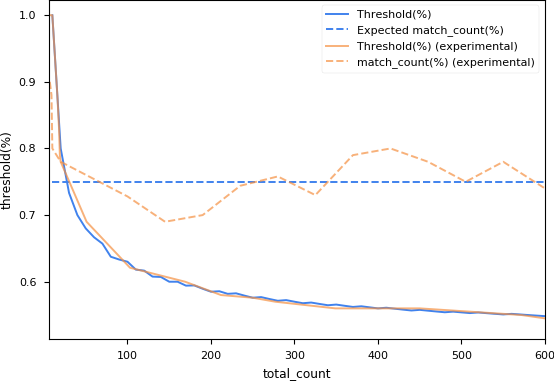
\includegraphics[width=\textwidth]{Figures/threshold_two-level.png}
    \caption{Portion of match\_count and \textit{threshold} for different total\_count to achieve the ownership confidence level 99\% ($\alpha_1=0.01$)}
    \label{fig:threshold-ownership}
\end{figure}

\Cref{fig:threshold-ownership} shows, for a fixed $\alpha_1=0.01$, the thresholds for different values of $total\_count$ as a fraction of $total\_count$ (continuous blue line).
The dashed blue line is the expected fraction of $match\_count$ out of $total\_count$ (75\%).
We can see that for the $total\_count$ larger than $\approx 30$ the previously mentioned condition is satisfied and the extraction algorithm can verify the ownership with a confidence level of 99\%. 
The statement is confirmed with the experimental results shown by the orange lines in the figure.
The experiments are run on Forest Cover Type data with fingerprint length $L=96$.
The $match\_count$ value in the experiments is $75\%(total\_count)\pm5\%$, according to the expectation. Furthermore, the lower limit for $total\_count$ to have 99\% confidence level for ownership is shown to be around 30. 
Therefore, \Cref{eq:ownership-verification} needs to be satisfied for the correct ownership verification.

\begin{equation}\label{eq:ownership-verification}
    2\eta/\gamma_1 > 30 (\alpha_1=0.01)
\end{equation}

For the real-life datasets with hundreds or thousands of tuples this is rather easy to achieve (e.g. for Forest Cover Type data, setting $\gamma_1=200$ results in $total\_count \approx 5,800$).

The second phase of detection algorithm - the fingerprint extraction - identifies each bit individually from the associated group of tuples. 
The process of comparing the matching bits to the threshold value is in this phase controlled by $\alpha_2$.
If the number of matches of a single bit value is larger than the threshold, the bit is decided to be that value (conditions in lines 11 and 13 of \Cref{alg:two-level-extraction}).

\begin{figure}
\centering
    \subfloat[$\alpha_2=0.01$]{{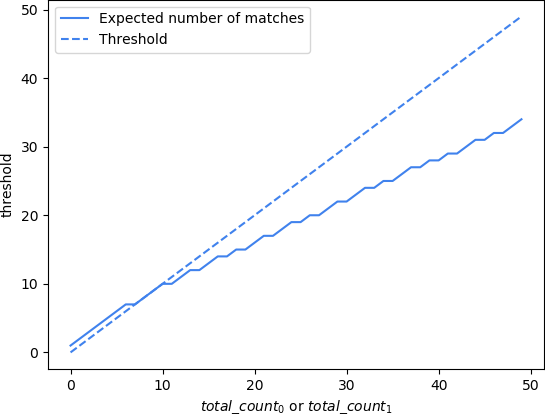
\includegraphics[width=6.7cm]{Figures/fingerprint-extraction-threshold-scrnsh.png} }}
    \qquad
    \subfloat[$\alpha_2=0.1$]{{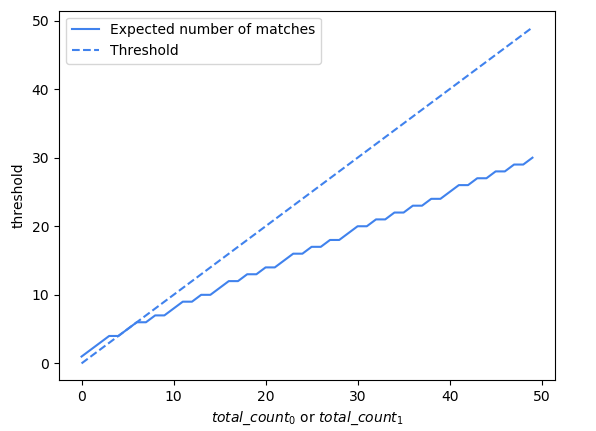
\includegraphics[width=6.7cm]{Figures/fingerprint-extraction-threshold-90.png} }}
    \caption{Threshold in subsets of unaffected marked data for different $total\_count_i$ to achieve confidence level of each bit of 99\% (a) and 90\% (b)}
    \label{fig:threshold-fingerprint-extraction}
\end{figure}

\Cref{fig:threshold-fingerprint-extraction} shows threshold values in a subset, depending on the total number of tuples in a subset. 
A dashed line represents the expected number of matches in a marked group of unaffected fingerprinted data.
We show the relation between thresholds and the number of matches for different levels of confidence - 99\% and 90\%.
Generally, the more tuples are selected into a subset, the more robust the fingerprint is. 
For reaching the confidence level of 99\%, $total\_count_i$  must be at least 8 for a trusted pattern to be found, while for 90\% confidence that lower limit is 4. 
Therefore, \Cref{eq:extraction-99} must be satisfied to obtain the successful marking pattern with confidence 99\% and \Cref{eq:extraction-90} with confidence 90\%.

\begin{equation}\label{eq:extraction-99}
    \eta/(\gamma_1 * L) > 7 (\alpha_2=0.01)
\end{equation}

\begin{equation}\label{eq:extraction-90}
    \eta/(\gamma_1 * L) > 3 (\alpha_2=0.1)
\end{equation}

In the real implementation $\eta/(\gamma_1 * L)$ should be rather larger than suggested in \Cref{eq:extraction-99,eq:extraction-90} because of the deviation introduced by random distribution of tuples into $L$ groups. 

\paragraph{}
The proposed technique has a limitation that it embeds the fingerprint in only one, initially chosen attribute. 
However, this approach is vulnerable to a vertical attack (attribute deletion attack) where the attacker can delete the fingerprint by removing the entire attribute. 
To avoid the possibility of such attack in multi-attribute datasets and for further experiments with this scheme, we slightly redesign the embedding and extraction process such that all attributes appear as candidates for marking. 
The simple modification is the reinterpretation of the term $LSB(r,j)$ in \Cref{alg:two-level-insertion}.
In this notation $LSB(r,j)$ represents the $j-th$ bit from the set of least significant bits available for marking of \textit{all} attribute values from the tuple $r$ (instead of only one predefined attribute).
Pseudo-randomness of this step ensures uniformly distributed marks over all attributes. 



\section{Fingerprinting categorical data}\label{subsec:fingerprinting-scheme-categorical}

We present two approaches to developing a technique that can be applied to both numerical and categorical data.
Both schemes use the processes of the AK Scheme for marking numerical values.
The first technique, a rather simplistic one, is based on a random choice of values to be marked and a random choice of a mark. 
In the second approach, we focus on keeping the semantic relations between the categorical data rather than purely randomly choosing the marks. 
The technique, however, relies on the availability of the original data, therefore, unlike the first scheme, it is not blind.
\paragraph{}
Another proposed technique for fingerprinting categorical data is \cite{Kieseberg2014fingerprinting}, where the $k$-anonymity pattern is used as a fingerprint. 
The number of $k$-anonymity patterns is limited and highly depends on the data and user-defined generalisation hierarchies, therefore also the number of distinct fingerprints is limited.
Furthermore, $k$-anonymity significantly changes the quality of the data. 
Since a subset of values is replaced by the respective value of the higher semantic category (e.g. Vienna->Austria), the informativeness of the data is lost.
Every buyer receives a distinct fingerprinted data copy, thus the quality of the data among the distributed copies differs significantly.
The technique lacks in implementation, therefore we do not include it in our analysis.

\subsection{Random mark choice}
\subsubsection{Methodology}
\paragraph{Insertion}
The approach for fingerprint embedding into the categorical data has the following steps:
\begin{enumerate}
    \item Label encoding all categorical values to obtain numerical data
    \item Fingerprint insertion algorithm of AK Scheme (Algorithm \ref{alg:AK-insertion})
    \item Applying modular arithmetic to fingerprinted numerical values of categorical data
    \item Decoding the values of categorical attributes
\end{enumerate}
The main idea of the approach is to convert categorical values to numerical values and treat them as any of the described methods for fingerprinting numerical data would. 
Assume that the attribute $A$ has $c$ different categorical values $C_0, ..., C_{c-1}$.
The label encoding model assigns each categorical value $C_i$ to the respective numerical value $i$.
After the fingerprint is embedded, the numerical values are being decoded back to the categorical values. 
A problem arises when a fingerprinted numerical value is not assigned to any of the categorical values in the encoding model because the range of values available in fingerprinting $2^\xi$, due to the binary representation, does not always correspond to the range of categorical values for an attribute.
The occurrence of such illegal values is possible when the fingerprint insertion algorithm marks a bit in the numerical representation of categorical value in such a way that the change of that bit transforms the numerical value to something that can't be decoded. 
For instance, assume that an attribute $A_1$ has 6 different categorical values ($c=6$), assigned by the encoding model to the numerical values $\{0,1,2,3,4,5\}$. 
Furthermore, assume $\xi=2$, and the insertion algorithm deciding to change the second least significant bit of value "4" somewhere within the dataset. 
The bit representation of the value $4_{10}=100_2$ will after marking be changed to $110_2$ which corresponds to $6$ in the decimal system, the value that is not assigned to any categorical value of attribute $A_1$. 
In general, the set of values of $A_1$ that can be obtained after embedding the fingerprint is $\{0,1,2,3,4,5,6,7\}$, where 6 and 7 are illegal values. 

Much bigger odds for a marked value to be out of bounds is in cases when the number of LSB-s available for fingerprinting $\xi$ is bigger than the length of bit representation the numerical values in label encoding model.
For example, assume $c = 4$, i.e. an attribute $A_2$ has 4 different values that are assigned to numerical values $\{0,1,2,3\}$, and $\xi = 3$. 
In case when insertion algorithm chooses, for example, value $2_{10}=10_2$ and its third least significant bit for fingerprinting, the resulting marked value is $110_2 = 6_{10}$, which does not have a corresponding categorical value in the encoding model. 
In general, after the fingerprint-embedding process, the domain of possible values of the attribute $A_2$ is $\{0,..,7\}$, where $\{4,5,6,7\}$ are not assigned to any original categorical value in our label encoding model. 

We solve the problem of illegal values in the fingerprinted dataset by applying modular arithmetic to the set of values obtained after fingerprinting. 
The final numerical value $x_i'$ of the attribute is given by $x_i' = x_i$ $mod$  $c$, where $x_i$ is the value after step 2 of the fingerprint-embedding process.
The modulo step in insertion algorithm for categorical data applied on $A_1$ would change the marked value $6_{10}=110_2$ to $6_{10} \mod 6 = 0_{10} = 000_2$. 

Finally, after removing the illegal values from the fingerprinted dataset, the numerical values are decoded to the categorical values. 

\paragraph{Detection}
Fingerprint detection process contains the following steps:
\begin{enumerate}
    \item Label encoding categorical values using the same model as in fingerprint insertion phase
    \item Fingerprint detection algorithm of AK Scheme (Algorithm \ref{alg:AK-detection})
\end{enumerate}

In the fingerprint detection process, it is again necessary to preprocess data by label encoding categorical values.
The encoding model needs to match the one from the insertion phase, otherwise, the detection process is disrupted.
After encoding categorical values, the AK detection algorithm \ref{alg:AK-detection} can be directly used to detect the malicious buyer.

\subsubsection{Properties and Discussion}
The properties of a detection algorithm for categorical data are essentially the same to the properties of AK detection algorithm, except that it is important to take into account the effects of modular arithmetic applied to the fingerprinted values where it is the case.
Consider the previous example with attribute $A_1$ where the fingerprint insertion algorithm changes the number representation $2_{10}=10_2$ of some categorical value to value $110_2 = 6_{10}$ by marking the third LSB and modulo operator application obtains the final marked value $6_{10} \mod 6 = 0_{10} = 000_2$. 
From this attribute value, the fingerprint bit cannot be correctly extracted anymore, therefore the detection algorithm is affected. 

The detection algorithm uses the technique called \textit{majority voting} for deciding the values of fingerprint bits, as discussed in \Cref{subsec:ak}.
This is the key to the property of the scheme that small errors in data do not prevent detecting the source of leakage. 
The effects of these small errors, i.e. values that are changed after inserting the fingerprint, are analysed in the context of attacks in \Cref{sec:Robustness}. 
Applying modulo to the values has the same effect on the detection process as purposely changing the values in fingerprinted data as part of a malicious attack (for example, bit flipping attack). 

 
The success of the detection process directly depends on the number of values that are a result of performing the modulo step in the insertion phase. 
This number is affected by the number of least significant bits we allow to change (parameter $\xi$) - larger $\xi$ leads to more frequent usage of modulo operation because the fingerprinted values more frequently get out of valid bounds. 
Since the detection process relies on multiple embeddings of a single fingerprint bit, having more marks in the dataset might assure that the fingerprint bits are detected correctly.
This is controlled by parameter $\gamma$ and the length of a fingerprint $L$.

\Cref{tab:detection-succ-german} presents the success of the detection algorithm for different values of parameters $\gamma$ and $\xi$. 
A fingerprint is in these experiments embedded in categorical values only.
Length of a fingerprint $L$ is set to 40.
The dataset used for experiments from \Cref{tab:detection-succ-german} is the German Credit data with 1000 entries and 21 attributes, out of which 14 are categorical. The dataset is described in \Cref{datasets}.
The results are based on 1000 runs of the algorithm for every parameter combination.

\begin{table}[ht]
    \centering
    \caption{Success of a detection algorithm of the fingerprinting scheme for categorical data using the German Credit dataset}
    \label{tab:detection-succ-german}
    \begin{tabular}{|c|r|r|r|r|}
    \hline
         & $\xi=1$ & $\xi=2$ & $\xi=4$ & $\xi=6$ \\
         \hline
         $\gamma=2$ & 99.8\% & 99.3\% & 56.4\% & 23.2\%\\
         \hline
         $\gamma=3$ & 94.7\% & 90.4\% & 17.3\% & 2.9\% \\
         \hline
         $\gamma=6$ & 30.0\% & 18.2\% & 0.3\% & 0\%\\
         \hline
         $\gamma=9$ &  2.9\% & 1.0\% & 0\% & 0\%\\
         \hline
         $\gamma=12$ & 0.1\% & 0\% & 0\% & 0\%\\
         \hline
    \end{tabular}
\end{table}

The detection algorithm performance significantly drops when either $\xi$ or $\gamma$ are increased. 
The expectation that the performance of the detection algorithm drops if more LSB-s are available for embedding the fingerprint (larger $\xi$) is confirmed by these experiments. 
\Cref{tab:german-credit} shows how many categorical attributes have a certain amount of different values in German Credit dataset. 
For instance, 3 out of 14 categorical attributes have 3 different values and therefore require only 2 bits to be encoded. 
An additional 10 attributes have up to 5 different values, therefore can be encoded by 3 bits. 


In the case where our insertion algorithm marks the 1st or the 2nd LSB of the value, the value obtained after fingerprinting will most likely be a modified numerical value that can be decoded back to a valid categorical value.
However, allowing e.g. the 4th significant bit to be marked in the insertion process opens more possibilities of obtaining values outside of the bounds, and modulo needs to be applied.
This results in the big decrease in the detection that can be seen in \Cref{tab:detection-succ-german} between $\xi=2$ and $\xi=4$. 
Applying modulo changes the marked value in the way that the detection algorithm can't extract the fingerprint bit correctly, leading to the impossibility of detecting a valid fingerprint. 
Generally, increasing $\xi$ leads to worse performance of the detection algorithm. 
A good choice for value of parameter $\xi$ depends very much on the dataset. 
One needs to inspect the dataset to see approximately how many different values the categorical attributes have, and set $\xi$ accordingly.
For example, if most of the categorical attributes have approximately 4 values, then $\xi$ should be at most 2 to keep the performance of the detection algorithm high. 
Generally, $\xi$ should be set to at most the number of bits needed to encode all the values of the attribute to their binary representations. 
The choice of parameter $\xi$ according to this will help in decreasing the loss in performance of the detection algorithm, but it generally cannot be completely avoided.
One of the reasons is that the choice of $\xi$ is limited to choosing the same value for the entire dataset, i.e. the same number of LSBs is available for fingerprinting in any of the attributes, no matter the size of their domains.
The optimal choice for $\xi$ from a detection performance point of view is then constrained by attributes with a small number of different values, while from the robustness point of view it is desired to have larger $\xi$, as discussed in detail in \Cref{sec:Robustness}. 
On the other hand, if the numbers of different values in all categorical attributes are not all power of two and $\xi$ not set according to the size of the smallest domain, there will always be even a minor possibility that the \textit{modulo} will be applied and will affect the detection algorithm. 

Besides the parameter $\xi$, the parameter $\gamma$ affects the performance of the detection algorithm, as shown in \Cref{tab:detection-succ-german} ($\gamma=2$ means that on average every second tuple is chosen for fingerprinting). 
Experiments show a significant decrease in performance when increasing $\gamma$. 
Increasing $\gamma$ means marking fewer tuples. Consequently, each fingerprint bit will be embedded in the data fewer times. 
This makes it harder for the detection algorithm to extract the correct value of a specific fingerprint bit when errors caused by the modulo operation are introduced. 
The design of our detection algorithm requires the perfect match of the fingerprint extracted by detection algorithm to some valid buyer's fingerprint, therefore only one falsely extracted fingerprint bit is enough for detection algorithm to fail. 
This is the reason for the success of 0\% for experiments with both high $\gamma$ and high $\xi$.

The issue that arises when fingerprinting dataset as small as German Credit data with only 1000 rows is that with $\gamma$ large enough, some fingerprint bits don't get embedded at all in the insertion process. 
Let us have an example where $\gamma=12$ and $L=40$. 
According to the parameters, $1000/\gamma \approx 83$ rows will be fingerprinted, and each fingerprint bit will be embedded into the dataset $83/40\approx2$ times. 
This number is approximate, and most importantly, averaged over all fingerprint bits. 
Since the choice of fingerprint bit to be embedded is completely independent and random in every step of the insertion algorithm, it is plausible to expect some bits being embedded 0 times.
This means that the detection algorithm will fail to extract the valid fingerprint from the unchanged fingerprinted dataset if the insertion process failed to embed all fingerprint bits at least once.
This observation is important to be noted when analyzing results from the \Cref{tab:detection-succ-german} because the success of the detection algorithm in small datasets is affected not only by errors caused by modulo operation but also by the failure of insertion algorithm to embed all of the fingerprint bits for larger $\gamma$.
To analyze these effects as separate cases, we define the following measures:
\begin{itemize}
    \item \textit{DFR} (Detection Fail Rate) - the number of fingerprint bits wrongly extracted because of the errors caused by modulo operation in the fingerprint detection process
    \item \textit{IFR} (Insertion Fail Rate) - the number of fingerprint bits that were not embedded at all in the fingerprint insertion process, and are therefore impossible to be extracted (unknown bit value)
    \item \textit{DIFF} - bit difference between the extracted fingerprint and the correct one; $DIFF = DFR + IFR$
\end{itemize}
\Cref{tab:detection-fail-rates} shows the rates obtained by the experiments shown in the \Cref{tab:detection-succ-german}, and presents a comparison of how much effect on the success of detecting the valid fingerprint is due to the modulo operation, and how much due to non-embedded bits. 
Rates in the table are the average values of rates from all 1000 runs. 
Insertion Fail Rate (\textit{IFR}) depends only on the number of dataset values being fingerprinted, i.e. parameter $\gamma$.
For $\gamma$ as small as two, a single fingerprint bit is embedded $1000/(\gamma * L) \approx 13$ times on average, and experimental results show that the insertion algorithm does not fail in embedding all of the fingerprint bits in any of the 1000 trials. 
The detection algorithm is, for $\gamma=2$, affected only by errors induced by modulo, and the fingerprint extracted by the algorithm and the correct one differ in only 0.002 bits on average.
For $\gamma = 12$ the \textit{IFR} raises up to $\approx5 / 40$, i.e. on average 5 out of 40 bits of the extracted fingerprint are incorrect.
From the experiments, we can see that in most of the cases $DFR$ is larger than $IFR$, i.e. errors in fingerprint extraction are mostly caused by applying modulo operation, except for small values of $\xi$. 

\begin{table}[ht]
    \centering
    \caption{Bit difference and the detection fail rates for the German Credit data}
    \label{tab:detection-fail-rates}
    \resizebox{\textwidth}{!}{
    \begin{tabular}{|c|r|r||r|r||r|r||r|r||r|r||r|}
    \hline
         & \multicolumn{2}{c||}{$\xi=1$} & \multicolumn{2}{c||}{$\xi=2$} & \multicolumn{2}{c||}{$\xi=4$} & \multicolumn{2}{c||}{$\xi=6$} &  \\
         \hline
         & $DIFF$ & $DFR$ & $DIFF$ & $DFR$ & $DIFF$ & $DFR$ & $DIFF$ & $DFR$ & $IFR$ \\
         \hline
          $\gamma=2$ & $ 0.002$& $  0.002$ & $ 0.007$ & $  0.007$ & $ 0.562$ & $  0.562$  &  $ 1.376$
             & $  1.376$ & 0\\
         \hline 
         $\gamma=3$ & $ 0.055$ & $  0.045$ & $ 0.100$ & $  0.090$  & $ 1.654$ & $  1.644$ & $ 3.203$ & $  3.193$
              & 0.010 \\
         \hline
         $\gamma=6$ & $1.170$ & $0.558$ & $1.642$ & $1.030$ & $5.603$ & $4.991$ & $7.842$  & $7.230$ & 0.612 \\
         \hline
          $\gamma=9$ & $3.615$ & $ 1.105$ & $4.256$ & $1.746$ & $9.206$ & $ 6.696$ & $11.498$ & $ 8.988$ & 2.510 \\
         \hline
         $\gamma=12$ & $6.462$ & $ 1.424$ & $
         7.190$ & $ 2.152$ & $11.935$ & $6.897$ &  $14.095$ & $9.057$ & 5.038 \\
         \hline
    \end{tabular}}
\end{table}


\Cref{tab:detection-succ-german-without-modulo} shows the experimental results of the success of the detection algorithm when modulo is not applied, but illegal numerical values are left in the fingerprinted dataset. 
Experiments are as well run on the German Credit dataset, with 1000 runs for each parameter value. 
This table highlights the case of having a small dataset. 
The results show how limited the choice of parameter $\gamma$ is in these cases. 

\begin{table}[ht]
    \centering
    \caption{Success of a detection algorithm using the German Credit dataset without applying modulo operation}
    \label{tab:detection-succ-german-without-modulo}
    \begin{tabular}{|c|c|c|c|c|c|}
    \hline
         $\gamma=2$ & $\gamma=3$ & $\gamma=6$ & $\gamma=9$ & $\gamma=12$ & $\gamma=15$\\
         \hline
         100\% & 99.0\% & 54.5\% & 7.6\% & 0.6\%  & 0\%\\
         \hline
    \end{tabular}
\end{table}

We repeat the experiments on another, larger dataset in order to examine the effects of modulo operation on the detection process, without other side effects such as the insertion algorithm failure.
For the experiments, we use Adult dataset. 
The dataset originally has 32,561 rows that contain missing values.
We will not examine dealing with missing values, so for the experiments, we use the subset of 30,162 rows that do not contain any missing values.
\Cref{tab:detection-succ-adult} shows the experimental results of the success of the detection algorithm to recognise the correct malicious buyer.
the fingerprint length \textit{L} is set to 80.
The results in \Cref{tab:detection-succ-adult} are the percentage of successfully detected fingerprints out of 1000 runs for every parameter combination.

\begin{table}[ht]
    \centering
    \caption{Success of the detection algorithm using Adult dataset}
    \label{tab:detection-succ-adult}
    \begin{tabular}{|c|r|r|r|r|}
    \hline
         & $\xi=1$ & $\xi=2$ & $\xi=4$ & $\xi=6$ \\
         \hline
         $\gamma=3$ & 100\% & 100\% & 100\% & 100\% \\
         \hline
         $\gamma=6$ & 100\% & 100\% & 100\% & 100\%\\
         \hline
         $\gamma=12$ & 100\% & 100\% & 100\% & 99.5\%\\
         \hline
         $\gamma=25$ & 100\% & 100\% & 95.8\% & 64.0\% \\
         \hline
         $\gamma=50$ & 95.6\% & 72.6\% & 25.2\% & 1.4\% \\
         \hline
         $\gamma=100$ & 14.2\% & 3.0\% & 0\% & 0\% \\
         \hline
    \end{tabular}
\end{table}

Comparing the results from \Cref{tab:detection-succ-german} and \Cref{tab:detection-succ-adult} it can be observed that the detection algorithm performance improved a lot by having a larger dataset. 
For low $\gamma$ the performance is perfect or close to perfect. 
Again, increasing $\xi$ leads to worse performance of the detection algorithm since the modulo operation is required more and fingerprint bits are wrongly detected. 
In \Cref{tab:adult-detection-rates} we can see that the extracted fingerprint is very "close" to the valid one. 
For instance, in the case of $\gamma=50$ and $\xi=2$, the performance of the algorithm drops to 72.6\%, but the bit difference between the extracted and real fingerprint is on average 0.31 (\Cref{tab:adult-detection-rates}, $DIFF$ rate), meaning that for most of the remaining 27.4\% runs of the algorithm, the fingerprints' bit difference is only in one single bit. 
In \Cref{tab:adult-detection-rates} we omitted the experiments where the detection success is 100\% since all the rates for those cases are 0.
In other cases, we can see that insertion fail rate $IFR$ is very small or zero, so most of the fingerprint detection failure is caused by modulo operation. 

\begin{table}[ht]
    \centering
    \caption{The detection fail rates for Adult data}
    \label{tab:adult-detection-rates}
    \resizebox{\textwidth}{!}{
    \begin{tabular}{|c|r|r||r|r||r|r||r|r||r|r||r|}
    \hline
         & \multicolumn{2}{c||}{$\xi=1$} & \multicolumn{2}{c||}{$\xi=2$} & \multicolumn{2}{c||}{$\xi=4$} & \multicolumn{2}{c||}{$\xi=6$} &  \\
         \hline
         & $DIFF$ & $DFR$ & $DIFF$ & $DFR$ & $DIFF$ & $DFR$ & $DIFF$ & $DFR$ & $IFR$ \\
         \hline
        $\gamma=25$ & $ 0$  & $  0$  & $ 0$ &$  0$  & $ 0.043$ & $  0.043$ & $ 0.431$ & $  0.431$ & 0 \\
         \hline
         $\gamma=50$ & $ 0.047$ & $  0.003$ & $ 0.310$ & $  0.266$ & $ 1.302$ & $  1.258$  & $ 3.987$ & $  3.943$ & 0.044 \\
         \hline
         $\gamma=100$ & $ 1.994$ & $  0.158$ & $ 4.086$ & $  2.250$ & $ 7.030$ & $  5.194$ & $ 12.228$ & $  10.392$ & 1.836 \\
         \hline
    \end{tabular}}
\end{table}


The problem of having illegal categorical values after the fingerprinting process is thwarted by the solution that introduces another problem - the weaker performance of the detection algorithm. 
Bad performance of the detection algorithm necessarily means that the presented fingerprinting scheme for categorical data is more susceptible to the attacks.
Small datasets are more vulnerable because of the possibility that the insertion algorithm fails to embed the fingerprint properly, not only in the context of categorical data but in general.
By careful dataset inspection and parameter tuning, both problems of small dataset and errors caused by modulo can be avoided. 
Lower \textit{L}, $\gamma$ and $\xi$ in general lead to better performance.

\paragraph{}
We saw that the number of LSB-s $\xi$ defines the quality of the scheme and that by choosing smaller $\xi$ we can minimise the error of the detection algorithm. 
In the discussion above, we use the fixed $\xi$ for all the attributes. 
However, we could modify this property such that each attribute $A_i$ is associated with own $\xi_i$ based on the number of distinct values of that attribute. 
This way we increase the robustness by setting particular $\xi_i$ values as high as possible, taking into account the upper limit that is defined by the number of distinct values in the attribute. 
For instance, changing only one LSB in the attribute with only three values, but allowing to change 5 LSB-s in attributes with $>40$ values. 

This approach is simplistic but effective. 
We will see in \Cref{sec:Robustness} the robustness analysis of the scheme and in \Cref{chapter:Utility} the utility analysis.
Another aspect that could be taken into account when designing a robust fingerprint technique is the semantic correlation between the categorical attributes. 
For instance, the fingerprint might be much more perceptible when there is a frequent number of occurrences of impossible or very unlikely combinations of attribute values due to marking.
This problem is addressed in the following section.


\subsection{Choosing a mark based on correlations in the dataset}
This approach addresses the problem of semantic relations between categorical attributes that can be disturbed by fingerprinting. 
Considering attributes independently of each other and embedding a random mark into a categorical value might lead to non-consistent records. 
A mark may introduce an uncommon or impossible combination of values in the data. 
As an example, let us consider a dataset containing attributes \textit{gender}, \textit{numberOfPregnancies}, etc. The attributes \textit{gender} and \textit{numberOfPregnancies} intuitively contain an impossible combination of values: (\textit{gender}:male, \textit{numberOfPregnancies}:1).
Another example is where the combination of values might be very uncommon. Take, for example, a medical dataset containing information about the patients suffering from Alzheimer's disease. The combination 
(\textit{alzheimersStage}:middle, \textit{employed}:yes) is very uncommon, but might be introduced by a random fingerprint mark.
With a dataset domain knowledge, these examples would be rather suspicious and thus perceptible. 
We aim to take into account the correlation between the values of different attributes and avoid uncommon combinations. 
\Cref{alg:cat-insertion} shows the pseudocode for the insertion algorithm of the scheme.

\subsubsection{Methodology}
\paragraph{Insertion}
\begin{algorithm}
  \KwIn{dataset $\mathcal{R}$ with scheme $(P, A_{0}, ..., A_{v-1})$, buyer $n$'s ID $id$}
  \KwOut{fingerprinted dataset $\mathcal{R'}$}
  fingerprint of buyer $n$: $\mathcal{F}(\mathcal{K},id)=\mathcal{H}(\mathcal{K}|id)$
  \\
  \ForEach{tuple $r \in \mathcal{R}$}
  {
    \If{$(\mathcal{S}_{1}(\mathcal{K}|r.P)$ mod $\gamma == 0)$}{
        attribute\_index $i = \mathcal{S}_2(\mathcal{K}|r.P)$ mod $v$
        \\
        \uIf{$A_i$ is categorical}{
            mask\_bit $x=0$ if $\mathcal{S}_3(\mathcal{K}|r.P)$ is even; $x=1$ otherwise \\
            fingerprint\_index $l=\mathcal{S}_4(\mathcal{K}|r.P)$ mod $L$
            \\
            fingerprint\_bit $f=f_l$\\
            mark\_bit $m=x \oplus f$ \\
            \If{m == 1}{
                neighbourhood = $select\_neighbours()$ \\
                target\_values, freq = $get\_frequencies(\text{neighbourhood})$\\
                $r.A_i = random(\text{target\_values}, weight=\text{freq})$
            }
        }
        \uElseIf{$A_i$ is numerical}{
            bit\_index $j=\mathcal{S}_3(\mathcal{K}|r.P)$ mod $\xi$
            \\
            mask\_bit $x=0$ if $\mathcal{S}_4(\mathcal{K}|r.P)$ is even; $x=1$ otherwise
            \\
            fingerprint\_index $l=\mathcal{S}_5(\mathcal{K}|r.P)$ mod $L$
            \\
            fingerprint\_bit $f=f_l$
            \\
            mark\_bit $m=x \oplus f$
            \\
            $LSB(j,r.A_i) = m$
        }
    }
  }
  \Return{$\mathcal{R'}$}
  \caption{Fingerprinting technique for categorical data: Insertion Algorithm}
  \label{alg:cat-insertion} 
\end{algorithm}

The insertion algorithm resembles the AK Scheme's insertion algorithm (\Cref{alg:AK-insertion}).
The creation of a fingerprint and the pseudorandom choice of tuples and attributes to be marked is the same.
In this scheme, the distinction is made based on whether a numerical or a categorical attribute is chosen for fingerprinting (line 5). 
In a case where the attribute is categorical, the next random value generated by a pseudorandom number generator $\mathcal{S}$ decides the value of a mask bit $x$. 
Furthermore, the next random value from the generator decides which fingerprint bit $f_l$ is going to be embedded. 
The mark bit $m$ is a result of an XOR operation between the mask and the fingerprint bit. 
In case the mark is 1, the attribute value will be marked. 
The lines 11 to 13 of \Cref{alg:cat-insertion} are specific for this scheme and contain the main part of this scheme.
Instead of marking the value to something random from the domain of the attribute, the idea is to choose a value taking into account the values of the other attributes in the tuple. 
This way, the algorithm avoids the combinations of values that are unlikely to appear in the dataset. 
We search for a neighbourhood of the observed tuple regarding all attributes but one that is being fingerprinted. 
We find the neighbours using the nearest neighbours algorithm with the Hamming distance. 
We let the user select whether the neighbourhood will be defined as a certain number of neighbours, $k$, or as the set of elements within the given distance $d$.
The parameters $k$ and $d$ are predefined by the user as well. 
After the neighbours are obtained, we observe the values in the attribute $A_i$ and sort them by their frequencies. 
The new value, i.e. the fingerprinted value is then a random value from the set of neighbours' values, where the random choice is weighted by values' frequencies. 
This technique is known in genetic algorithms as a fitness proportionate selection, or roulette wheel selection, a genetic operator used for selecting potentially useful solutions for recombination.
Fingerprinting process of numerical values follows the steps of the AK Scheme. 

\paragraph{Detection}
The pseudocode for the detection algorithm is shown in \Cref{alg:cat-detection}.

\begin{algorithm}
  \KwIn{fingerprinted dataset $\mathcal{R'}$ with scheme $(P, A_0, ..., A_{v-1})$, original dataset $\mathcal{R}$ with scheme $(P,A_0,...,A_{v-1}$}
  \KwOut{suspected buyer's ID $id$}
  fingerprint template $\mathcal{F}=(f_0,...,f_{L-1})=(?,...,?)$  \\
  $count[i][0]=count[i][1]=0$ \textbf{for} $i=0$ to $L-1$\\ 
  \ForEach{tuple $r \in R'$}
  {
    \If{$\mathcal{S}_1(\mathcal{K},r.P)$ mod $\gamma==0$}
    {
        attribute\_index $i=\mathcal{S}_2(\mathcal{K},r.P)$ mod $v$\\
        \uIf{$A_i$ is categorical}{
            mask\_bit $x=0$ if $\mathcal{S}_3(\mathcal{K},r.P)$ is even; $x=1$ otherwise\\
            \uIf{$r.A_i$ is different from the original}{
                mark\_bit $m = 1$
            }
            \uElse{
                mark\_bit $m= 0$
            }
            fingerprint\_index $l=\mathcal{S}_4(\mathcal{K},r.P)$ mod $L$\\
        }
        \uElseIf{$A_i$ is numerical}{
        bit\_index $j=\mathcal{S}_3(\mathcal{K}, r.P)$ mod $v$\\
        mark\_bit $m=LSB(j, r.A_i)$\\
        mask\_bit $x=0$ if $\mathcal{S}_4(\mathcal{K},r.P)$ is even; $x=1$ otherwise\\
        fingerprint\_index $l=\mathcal{S}_5(\mathcal{K},r.P)$ mod $L$\\
        }
        //update the votes\\
        fingerprint\_bit $f=m \oplus x$\\
        $count[l][f]++$ 
    }
  }
  //recover the fingerprint\\
  \For{$l=0$ to $L-1$}
  {
    \If{$count[l][0]+count[l][1]==0$}
    {
        \Return{\textit{none suspected}}
    }
    $f_l=0$ if $count[l][0]/(count[l][0]+count[l][1])>\tau$\\
    $f_l=1$ if $count[l][1]/(count[l][0]+count[l][1])>\tau$\\
    \Return{\textit{none suspected}} otherwise
  }
  $\mathcal{F}=(f_0,...,f_{L-1})$\\
  $id=detect(\mathcal{F,K},L, N)$\\
  \uIf{$id\geq0$}
  {
    \Return{$id$}
  }
  \Else
  {
    \Return{\textit{none suspected}}
  }
  \caption{Fingerprinting technique for categorical data: Detection Algorithm}
  \label{alg:cat-detection}
\end{algorithm}

Similarly to the AK's detection algorithm (\Cref{alg:AK-detection}), the algorithm starts by initializing the fingerprint template and the votes for fingerprint bit values. 
We then find the tuples and attributes that should have been fingerprinting according to the same pseudorandom sequence as in the insertion algorithm. 
For categorical attributes, the fingerprint extraction is described from line 7 to 12. 
We retrieve the mask bit $x$.
Next, to find the value of the mask bit $m$, it is necessary to compare the suspected fingerprinted dataset to the original. 
If the corresponding value is different from the original, then the value $m$ was 1 in the insertion algorithm, otherwise 0. 
Furthermore, we find the fingerprint bit index $l$ as the next random value in the pseudorandom sequence generator.
The lines 13 to 17 contain the extraction from the numerical values which is the same as in the extraction algorithm of the Ak Scheme.
The lines 18 to 38 are common for both categorical and numerical data and follow the steps from the detection algorithm of the AK Scheme. 

\subsubsection{Discussion}
Neighbourhood search is implemented in two different ways and is left to the user to decide which one to use for the specific case. We allow searching for a fixed number of neighbours, $k$, or searching for neighbours within a predefined distance $d$. 
The choice between the approach, as well as setting the parameters $k$ and $d$ requires some expert knowledge about the dataset. 
In case of an approach based on selecting a fixed number of neighbours, it is important to handle the neighbours with the same distances deterministically. We solve this in the following way: first, we choose the $k$ neighbours, then find the maximum distance within the neighbours and select all elements outside of the neighbourhood with the same distance. 
Therefore, it might be the case where the neighbourhood is extended to more than $k$ elements.

The set of attributes included in the neighbourhood selection do not have to be the whole set of attributes of the dataset. 
This can be set by the user who has insights into the data and has the knowledge about the highly related attributes. 

The final choice of the mark could be ambiguous if we would always choose the most frequent ones, in cases when we have multiple values with the same frequencies. 
For that reason we choose to select the new value pseudorandomly, weighted by the frequencies. This way the whole set of values from the neighbourhood have a chance to be selected, while the most frequent one will be selected with the highest probability.



\section{Summary}
In this chapter we have presented three common fingerprinting techniques for fingerprinting relational datasets, the AK Scheme in \Cref{subsec:ak}, Block Scheme in \Cref{subsec:block-oriented-scheme} and Two-level Scheme in \Cref{sec:two-level-fp}. 
These techniques have in common the usage of cryptographically secure structures and algorithms, i.e. cryptographic pseudo-random sequence generator and cryptographic hash function. They are used for creating the buyers' fingerprints because of security reasons since they must remain secret to everyone except the owner of the dataset. 
These techniques are limited to application on numerical values in the data. 
Furthermore, two fingerprinting techniques for non-numerical data are introduced in \Cref{subsec:fingerprinting-scheme-categorical}.
Both techniques extend the AK Scheme such that the same algorithmic steps are used for fingerprinting the numerical part of the data. 
The first scheme follows the pseudo-random pattern of choosing marks for categorical values.
In the second scheme, the solution goes towards preserving the correlations between the categorical values and marks the values in a way that no uncommon combinations of values occur in the final fingerprinted copy of the dataset.

These techniques are the basis of the analysis in the following chapters. The techniques are susceptible to attempts of a malicious buyer to destroy the fingerprint from the dataset. 
In the next chapter, we analyse how robust these techniques are under certain types of attacks.


\chapter{Robustness of fingerprinting techniques against attacks}\label{sec:Robustness}

\section{Experimental setup}
\subsection{Robustness measures}
Fingerprinting schemes should be robust against different attempts to prevent the correct detection of the fingerprint.
Modifying, deleting and adding the values to the fingerprinted data, that can be both benign updates and malicious attacks, can modify or erase the fingerprint. 
A robust fingerprinting scheme should make it hard for the attacker to erase the fingerprint, to modify it in the way that an innocent buyer is implicated as a traitor, or to modify unmarked data such that a valid fingerprint is detected.

In further sections we analyse robustness fingerprinting schemes against different attacks using robustness measures proposed in \cite{li2005fingerprinting}:
\begin{itemize}
  \item \textbf{Misdiagnosis false hit} $(fh^D)$: The probability of detecting a valid fingerprint from data that has not been fingerprinted.
  \item \textbf{Misattribution false hit} $(fh^A)$: The probability of detection an incorrect but valid fingerprint from fingerprinted data.
  \item \textbf{False negative} $(fn)$: The probability of detecting no valid fingerprint from fingerprinted data.
  \item \textbf{False miss} $(fm)$: The probability of failing to detect an embedded fingerprint correctly. False miss rate is the sum of the false negative and misattribution false hit rates, i.e. $fm=fh^A+ fn$.
\end{itemize}

\subsection{Datasets}\label{datasets}
We use three different datasets for the experiments on fingerprint robustness and quality effects on fingerprinted datasets in the following sections obtained from the UCI Machine Learning repository \cite{Dua:2019}:
\begin{itemize}
    \item Forest Covertype dataset\footnote{\url{https://archive.ics.uci.edu/ml/datasets/covertype}}
    \item German Credit Data\footnote{\url{https://archive.ics.uci.edu/ml/datasets/statlog+(german+credit+data)}}
    \item Adult dataset (train data)\footnote{\url{https://archive.ics.uci.edu/ml/datasets/adult}}
\end{itemize}
\paragraph{Forest Cover Type}
The dataset contains measurements related to the forest cover originally obtained from US Geological Survey (USGS) and US Forest Service (USFS) data.
This dataset is chosen due to its desired properties of containing multiple integer-valued attributes, because of its size and because its intended purpose is the classification problem with target \textit{Cover\_Type}. 
This dataset is often used for experiments in watermarking and fingerprinting literature \cite{agrawal2003watermarking,li2005fingerprinting}, therefore using this dataset gives the possibility of comparing our results with previous work.
The dataset has 581,012 rows, each with 54 attributes and no primary key. 
For fingerprint insertion, an extra attribute - \textit{id} is added to serve as the primary key, since the chosen fingerprinting techniques require the presence of the primary key for fingerprint embedding. 
44 out of a total of 54 attributes of the dataset contain binary values. 
We use the remaining 10 integer-valued attributes for embedding fingerprints.
Binary attributes are a result of one-hot encoding, therefore changing one value from 0 to 1 or vice versa would require changing another attribute's value to retain the structure. The binary attributes of Forest dataset are excluded because of this high correlation that defines different properties compared to the numerical values in the context of fingerprinting. 
In \Cref{table:forest-attr}, the information about the attributes is given.

\begin{table}[ht]
\centering
\caption{Attributes of the Forest Cover Type dataset}
\label{table:forest-attr}
\resizebox{\textwidth}{!}{
\begin{tabular}{|c|c|c|} 
 \hline
 Name & Description & Type\\
 \hline
 \hline
 Elevation  & Elevation in meters & Int\\
 \hline
 Aspect  & Aspect in degrees azimuth & Int\\
 \hline
 Slope  & Slope in degrees & Int\\
 \hline
 Horizontal\_Dist\_To\_Hydrology  & Horizontal distance to nearest surface water features & Int \\
 \hline
 Vertical\_Dist\_To\_Hydrology  & Vertical distance to nearest surface water features & Int\\
 \hline
 Horizontal\_Dist\_To\_Roadways  & Horizontal distance to nearest roadway  & Int\\
 \hline
 Hillshade\_9am & Hillshade index at 9am, summer solstice & Int\\
 \hline
 Hillshade\_Noon & Hillshade index at noon, summer solstice  & Int\\
 \hline
 Hillshade\_3pm & Hillshade index at 3pm, summer solstice  & Int \\
 \hline
 Horizontal\_Dist\_To\_Fire\_Points & Horizontal distance to nearest wildfire ignition points  & Int\\
 \hline
 Wilderness\_Area (4 columns) & Wilderness area designation & Binary\\
 \hline
 Soil\_Type (40 columns) & Soil Type designation & Binary\\
 \hline
 Cover\_Type & Forest Cover Type designation & Int \\
 \hline
\end{tabular}}
\end{table}

\paragraph{German Credit Data}
The dataset describes persons by attributes containing some personal information and classifies them as good or bad in terms of risk for the credit defaulting. 
The dataset has 1000 rows, 20 attributes and one target attribute.
13 out of 20 attributes in this dataset, as well as the target attribute in this dataset,  are categorical and we use this dataset to analyse the performance of the fingerprinting scheme for categorical data described in \Cref{subsec:fingerprinting-scheme-categorical} and for experiments on the impact of fingerprinting to a learning task in \Cref{sec:Learning}. 
The dataset is also chosen for its size. 
Because it is considerably smaller than Forest Cover Type, there is a possibility that the size of a dataset can affect the performance of fingerprinting algorithms.
Detailed information about the attributes in the dataset is given in \Cref{tab:german-credit}.

\begin{table}[ht]
    \centering
     \caption{Attributes of the German Credit dataset}
    \label{tab:german-credit}
    \begin{tabular}{|c|c|c|c|}
    \hline
        Name & Description & Type & \#values \\
    \hline
    \hline
         Attr.1 & Status of existing checking account & Categ. & 4 \\
         \hline
         Attr.2 & Duration in month & Int & \\
         \hline
         Attr.3 & Credit history & Categ. & 5\\
         \hline
         Attr.4 & Purpose & Categ. & 11 \\
         \hline
         Attr.5 & Credit amount & Int & -\\
         \hline
         Attr.6 & Savings account/bonds & Categ. & 5\\
         \hline
         Attr.7 & Present employment since & Categ. & 5\\
         \hline
         Attr.8 & Installment rate of disposable income (\%) & Int & -\\
         \hline
         Attr.9 & Personal status and sex & Categ. & 5 \\
         \hline
         Attr.10 & Other debtors/guarantors & Categ. & 3\\
         \hline
         Attr.11 & Present residence since & Int & -\\
         \hline
         Attr.12 & Property & Categ. & 4\\
         \hline
         Attr.13 & Age in years & Int & -\\
         \hline
         Attr.14 & Other installment plans & Categ. & 3\\
         \hline
         Attr.15 & Housing & Categ. & 3\\
         \hline
         Attr.16 & Number of existing credits at this bank & Int & -\\
         \hline
         Attr.17 & Job & Categ. & 4\\
         \hline
         Attr.18 & Number of liable people & Int & -\\
         \hline
         Attr.19 & Telephone & Bin & 2 \\
         \hline
         Attr.20 & Foreign worker & Bin & 2 \\
         \hline
         Target & Good or bad credit risks & Bin & 2\\
         \hline
    \end{tabular}
\end{table}

\paragraph{Adult dataset}
The dataset contains information about people such as their age, workclass, education, etc. and a target attribute whether a person makes at least \$50K per year or less than \$50K.
This dataset contains 15 attributes in 30,162 samples of training data (after removing samples containing missing values), where the attributes are both numerical and categorical (five continuous numerical and ten categorical). 
The same as German Credit dataset, we use this dataset to analyse the performance of fingerprinting scheme for categorical data in \Cref{subsec:fingerprinting-scheme-categorical} and for experiments on the impact of fingerprinting to a learning task in \Cref{sec:Learning}. \Cref{tab:adult_attributes} describes the attributes of the Adult dataset.

\begin{table}[ht]
    \centering
    \caption{Attributes of the Adult dataset}
    \label{tab:adult_attributes}
    \begin{tabular}{|c|c|c|}
    \hline
         Name & Type & \#values \\
         \hline
         age & Continuous & - \\
         \hline
         workclass & Categorical & 8 \\
         \hline
         fnlwgt & Continuous & -\\
         \hline
         education & Categorical & 16 \\
         \hline
         education-num & Continuous & 16 \\
         \hline
         marital-status & Categorical & 7 \\
         \hline
         occupation & Categorical & 14 \\
         \hline
         relationship & Categorical & 6 \\
         \hline
         race & Categorical & 5 \\
         \hline
         sex & Categorical & 2 \\
         \hline
         capital-gain & Continuous & - \\
         \hline
         capital-loss & Continuous & - \\
         \hline
         hours-per-week & Continuous & - \\
         \hline
         native-country & Categorical & 41 \\
         \hline
         income & Categorical & 2 \\
         \hline
    \end{tabular}
\end{table}

\subsection{Attacks}
In the following sections we discuss and analyse the robustness of the fingerprinting schemes, described in \Cref{sec:Fingerprinting}, against the following attacks:
\begin{itemize}
    \item Subset attack - the attacker releases only a subset of the dataset rows as an attempt to erase the fingerprint
    \item Superset attack - the attacker adds additional rows to the original dataset and mixes them with the original rows
    \item Bit-flipping attack - the attacker flips arbitrary bits in the dataset in an attempt to erase the fingerprint
    \item Additive attack - the attacker inserts additional fingerprint to the data, claiming the ownership
    \item Collusion attack - multiple buyers compare their dataset copies and create a new copy in an attempt to erase the fingerprint of every buyer in the collision
\end{itemize}

\section{Misdiagnosis false hit}
In this section, we will analyse the misdiagnosis false hit rate of different fingerprinting schemes. 
This robustness measure differs from the others in a way that it does not measure the success of a malicious attack or benign updates on the dataset. 
In contrast to the ability of the detection algorithm to detect the correct fingerprint from the pirated (and fingerprinted) data, the fingerprinting scheme may also, purely by chance, extract a valid but incorrect fingerprint from unmarked data.
This phenomenon is measured by misdiagnosis false hit rate.

\subsection{AK Scheme}\label{subsubsec:misdiagnosis-ak}
Assume that the detection algorithm from the unmarked data extracts a potential fingerprint $f=(f_0,...,f_{L-1})$, i.e. some bit string of length \textit{L}. 
Furthermore, assuming that a single fingerprint bit $f_i$ is extracted from the dataset multiple times, it is decided to be a single value (0 or 1) if that value is extracted more than $\tau\omega_i$, where $\omega_i$ is the number of times $f_i$ is extracted.
Due to the use of pseudo-random mask bits in this scheme, each time $f_i$ is extracted, it will be extracted as 0 or 1 with probability 0.5, which is modelled as an independent Bernoulli trial.
Once when the detection algorithm is done processing the dataset, the probability of the value of one fingerprint bit $f_i$ of the extracted potential fingerprint $f$ being 0 is $B(\lfloor\tau\omega_i\rfloor;\omega_i,0.5)$, and the same probability stands for $f_i$ being 1. 
Therefore, the algorithm detects the potential fingerprint with the probability $\prod_{i=0}^{L-1}2B(\lfloor\tau\omega_i\rfloor;\omega_i,0.5)$.
The probability that the extracted fingerprint is matching one of the $N$ valid ones equals to choosing $N$ bit strings out of $2^L$ possible ones: $N/2^L$.
Now the overall misdiagnosis false hit rate is 
\begin{equation}
    fh^D = \frac{N}{2^L}\prod_{i=0}^{L-1}2B(\lfloor\tau\omega_i\rfloor;\omega_i,0.5)
\end{equation}
and after $2^L$ cancels out 
\begin{equation}
    fh^D = N\prod_{i=0}^{L-1}B(\lfloor\tau\omega_i\rfloor;\omega_i,0.5)
\end{equation}
The misdiagnosis false hit rate is exponentially dependant on length of the fingerprint \textit{L}. The rate can be reduced by increasing \textit{L}. \Cref{table:misdiagnosis-fh} shows the misdiagnosis false hit rate under different values of $L$ and $\omega_i \approx \{100,50\}: \forall i \in \{0,...,L-1\}$, where $N=100$ and $\tau=0.5$ are fixed values.

\begin{table}[ht]
\centering
\caption{Misdiagnosis false hit rate for the AK Scheme}
\label{table:misdiagnosis-fh}
\begin{tabular}{|c|c|c|c|c|c|} 
\hline
 $L$ & 8 & 16 & 32 & 64 & 128 \\
 \hline
 $fh^D (\omega_i=100)$ & 0.7208 & 0.0052 & $2.70\times 10^{-7}$ & $7.30\times 10^{-16}$ & $5.31\times 10^{-33}$ \\
 \hline
 $fh^D (\omega_i=50)$ & 0.9151 & 0.0084 & $7.01\times 10^{-7}$ & $4.92\times 10^{-15}$ & $2.42\times 10^{-31}$\\
 \hline
\end{tabular}
\end{table}

We can see that for $L \gg log(N)$ we can almost completely avoid the misdiagnosis false hit ($fh^D\simeq0$) and by this rule, we will be choosing the values for $L$ in further analysis and experiments in this thesis.

\subsection{Block Scheme}
The probabilistic model for the misdiagnosis false hit is the same as in the case of AK Scheme, so for analysis on this topic, we refer to \Cref{subsubsec:misdiagnosis-ak}.

\subsection{Two-level Fingerprinting Scheme}
Two-level Fingerprinting Scheme detects the detected fingerprint in multiple phases. 
The extraction starts with ownership verification followed by fingerprint extraction and fingerprint verification. 
The detection algorithm goes to the extraction phase only if the ownership is verified, suggesting that first, we have to take into account the probability of passing the first phase of detection. 

Let us assume that the input to the detection algorithm is an unmarked dataset of size $\eta$. 
We set $\alpha_1=\alpha_2=\alpha_3=0.01$ and choose arbitrary $\gamma_1$ and $\gamma_2$. 
The subroutine \textit{detect} \ref{alg:detect-subroutine} counts the amount of tuples that should have been marked with 1 ($total\_count_1$) and with 0 ($total\_count_0$) in the embedding process.
Due to uniformly distributed output of the hash function $\mathcal{H}$, the approximate value of both $total\_count_1$ and $total\_count_0$ will be:
\begin{equation}
    total\_count_1 \approx total\_count_0 \approx \eta/\gamma_1
\end{equation}
Furthermore, the subroutine counts number of matches of chosen bits with the suggested values ($match\_count_1$ and $match\_count_0$).
Again, assuming the uniformity of the hash function:
\begin{align}
    &match\_count_1 \approx total\_count_1 / 2 \\
    &match\_count_0 \approx total\_count_0 / 2
\end{align}

To pass the ownership verification test, the total number of matches has to satisfy the condition:
\begin{equation}
    match\_count > threshold(total\_count, \alpha_1)
\end{equation}
where $match\_count = match\_count_1 + match\_count_0$ and $total\_count = total\_count_1 + total\_count_0$.
Therefore, for the ownership verification with confidence 99\% the following has to hold:
\begin{equation}
    \frac{threshold(total\_count, 0.01)}{total\_count} < 0.5
\end{equation} 
The value of this portion is shown in \Cref{fig:threshold-ownership} with the solid blue line. 
Even for very big $total\_count$, the threshold portion very slowly approaches 0.5. 
Thus, the ownership is very unlikely to be falsely verified in the unmarked dataset.

The extraction algorithm does not continue if ownership is not verified, therefore the scheme is extremely robust against misdiagnosis false hit.


\subsection{Fingerprinting scheme for categorical data}
The probabilistic model for the misdiagnosis false hit for the fingerprinting scheme for the categorical data is the same as in the case of AK Scheme. For the analysis, we refer to \Cref{subsubsec:misdiagnosis-ak}.

\section{Subset attack} \label{subsec:subset-attack}
In the attempt to erase the fingerprint from the dataset, the attacker may release only a subset of tuples of a fingerprinted dataset. 
This is called a subset attack. 
In our attack model, we assume the attacker selects each tuple independently with probability \textit{p} to include it in the pirated dataset. 
We also assume no other updates on the dataset are applied and no other attacks performed. 

\subsection{AK Scheme}\label{subsubsec:subset-ak}
A subset attack succeeds when all embedded bits for at least one fingerprint bit are deleted. Assuming that each fingerprint bit $f_i$ is embedded $\omega_i$ times, then the probability that all embedded bits for $f_i$ are deleted is $(1-p)^{\omega_i}$. The probability that no valid fingerprint will be detected from the dataset is then 
\begin{equation} \label{eq:subset-attack-ak}
    fm = 1 - {\prod_{i=0}^{L-1}(1-(1-p)^{\omega_i})}.
\end{equation}

Table \ref{table:subset-attack-ak} shows the probability of a successful attack for different parameter $\gamma$ values. 
$p'=1-p$ denotes the probability that a single tuple is deleted, i.e. the approximate percentage of deleted tuples since the choice of deletion is made independently by the attacker. 
We set $\eta = 581,012$, $v=10$ (according to the properties of Forest Cover Type dataset that we use in empirical evaluation), $\xi=4$ and $L=96$.
We can see from the table that the subset attack only gets to the reasonable level of probability for success with more than at least 90\% deleted tuples, depending on $\gamma$. 
We have to take into account that as few as 1\% of the tuples in this example is around 5810 tuples, which for the attacker might still be the acceptable amount of tuples to release without authorisation and perform the successful subset attack if $\gamma$ is set high enough ($\gamma \geq 25$). 
In those cases where $p'$ is large, $\gamma$ should be set to the smaller value, since the probability for a successful subset attack decreases when $\gamma$ decreases for the same $p'$.
Therefore, we adapt $\gamma$ to prevent the subset attack.

\begin{table}[ht]
\centering
\caption{Probability of a successful subset attack on the AK Scheme}
\label{table:subset-attack-ak}
\begin{tabular}{|c|c|c|c|c|c|} 
 \hline
 & \textbf{$p'=70\%$} & \textbf{$p'=80\%$} & \textbf{$p'=90\%$} & \textbf{$p'=95\%$} & \textbf{$p'=99\%$}\\
 \hline
 $\gamma=6$ & 0 & 0 & 0 & 0 & 0.0038 \\
 \hline
 $\gamma=12$ & 0 & 0 & 0 & $5.6881 \times 10^{-10}$ & 0.4555 \\
 \hline
 $\gamma=25$ & 0 & 0 & $8.1088\times 10^{-10}$ & 0.0004 & 0.99985 \\
 \hline
 $\gamma=50$ & 0 & 0 & 0.0003 & 0.1761 & 1 \\
 \hline
  $\gamma=100$ & $4.877\times 10^{-8}$ & 0.0001 & 0.1586 & 0.9892 & 1 \\
 \hline
\end{tabular}
\end{table}


\paragraph{Experiments}
To present empirically the success of the subset attack, we performed the attack on the Forest dataset with $\eta = 581,012$ and $v=10$ using different parameter settings. 
The parameters are chosen the same way as shown in table \ref{table:subset-attack-ak} to be able to compare theoretical results with the empirical.
The experimental results are shown in table \Cref{table:subset-attack-ak-emp}.
Every experiment is run 500 times and parameters are set as presented in the table. 
We set $L=96$ and $\xi=4$ where the later does not affect the success of the subset attack.

We can see from the table \Cref{table:subset-attack-ak-emp} that the results roughly match our analysis. 
The best rate of success has the attacks where most of the tuples are deleted ($>$95\%) and the percentage of fingerprinted tuples is low ($\gamma$ is high). 
Therefore, we can argue that the AK Scheme is robust against subset attacks. 

\begin{table}[ht]
\centering
\caption{Experimental results of a subset attack success rate on the AK Scheme, using the Forest dataset}
\label{table:subset-attack-ak-emp}
\begin{tabular}{|c|c|c|c|c|c|} 
 \hline
 & \textbf{$p'=70\%$} & \textbf{$p'=80\%$} & \textbf{$p'=90\%$} & \textbf{$p'=95\%$} & \textbf{$p'=99\%$}\\
 \hline
 $\gamma=6$ & 0 & 0 & 0 & 0 & 0.004 \\
 \hline
 $\gamma=12$ & 0 & 0 & 0 & 0 & 0.5 \\
 \hline
 $\gamma=25$ & 0 & 0 & 0 & 0 & 1.0 \\
 \hline
 $\gamma=50$ & 0 & 0 & 0.002  & 0.194 &  1.0 \\
 \hline
  $\gamma=100$ & 0 & 0 & 0.20 & 0.9975 &  1.0 \\
 \hline
\end{tabular}
\end{table}


Note that our original dataset did not have a primary key. 
Instead, we added the attribute \textit{Id} to serve as the primary key. 
For simplicity purposes, the $Id$ values in the experiments are represented by the sequence number of the tuple.
Furthermore, although during subset attack the attacker removes some tuples, we assume that the primary key of every preserved tuple will not change.
In case the primary key is removed or manipulated, the recreation of one is crucial for the defence against the subset attack.
Availability of the original dataset simplifies the process of recreating the primary key. 
A simple matching algorithm can be applied to the suspect dataset that compares values of bit positions which are not being selected for marking in the fingerprinting process to the same set of bit positions in the original data. 
This approach might be flawed by having multiple primary key value candidates for a single tuple. 
In that case, the additional decision step based on the similarity of the bits used for marking can be applied.
Alternatively, the virtual primary key construction technique proposed in \cite{li2003constructing} can be used to generate the primary keys and does not require the presence of the original dataset. 
Primary keys are generated from the unmarked parts or data and the owner's secret key using a cryptographic hash function. Without knowing the secret key, recreating the primary key values is unfeasible. 

\subsection{Block Scheme}
For the Block Scheme detection algorithm, it is crucial to have the same number of tuples and attributes and their correct order in the suspicious database. Otherwise, we cannot detect a valid fingerprint. 
When the attacker removes the chosen tuples, the defence has to replace the deleted one with the corresponding ones from the original dataset. 
In our analysis we formulate the deletion of each tuple as an independent trial with two possible outcomes whose probabilities remain the same through the trials (\textit{Bernoulli trial}). Furthermore, with $B(k;n.p)$ we denote the probability of having at least $k$ successes in $n$ trials with probability $p$ of success.  
The detection algorithm will be able to detect the correct fingerprint if every fingerprint bit $f_i$ occurs at least $\lfloor\tau\omega_i\rfloor$ times in the suspicious dataset.
It means that at least $\lfloor(1-\tau)\omega_i\rfloor$ embedded bits for some fingerprint bit have to be deleted for the attack to succeed.  
If the attacker examines each tuple independently and selects it for inclusion in the pirated database (i.e. deletes it with probability $p'=1-p$), the probability that the fingerprint bit $f_i$ cannot be detected is $B(\lfloor(1-\tau)\omega_i\rfloor;\omega_i,p')$.
Note that each fingerprint bit in the Block Scheme is embedded either $\omega$ or $\omega-1$ times, so we approximate this value to $\omega$ for the convenience.
Then the probability that the detection algorithm will fail to extract the fingerprint is 
\begin{equation}
    fm=1-(1-B(\lfloor(1-\tau)\omega_i\rfloor;\omega_i,p'))^L
\end{equation}

Table \ref{table:subset-attack-block} shows the probabilities of successful subset attack under different values of parameter $\beta$ and different probabilities $p'$. For calculations we use dataset of size $\eta = 581,012$ and $v=10$ attributes, for purpose of comparing these results with experimental results.
The other parameters are set as follows: $\xi=3$, $L=96$ and $\tau=0.5$.

\begin{table}[ht]
\centering
\caption{Probability of a successful subset attack on the Block Scheme}
\label{table:subset-attack-block}
\begin{tabular}{|c|c|c|c|c|} 
 \hline
 & \textbf{$p'=30\%$} & \textbf{$p'=40\%$} & \textbf{$p'=45\%$} & \textbf{$p'=50\%$}\\
 \hline
 $\beta=5$ & 0 & 0 & 0 & 1.0 \\
 \hline
 $\beta=10$ & 0 & 0 & 0.001 & 1.0 \\
 \hline
 $\beta=15$ & 0 & $6.8233\times10^{-7}$ & 0.2320 & 1.0 \\
 \hline
 $\beta=20$ & 0 & $9.7949\times10^{-4}$ & 0.8301 & 1.0\\
 \hline
  $\beta=30$ & $2.0832\times10^{-7}$ & 0.2151 & 0.9998 & 1.0 \\
 \hline
\end{tabular}
\end{table}

\paragraph{Experiments}
We present the empirical results of the success of a subset attack on the Block Scheme. 
The experiments are run on Forest dataset of size $\eta = 581,012$ and $v=10$ attributes, with parameters $\xi=3$, $L=96$ and $\tau=0.5$.
We measure success of the attack for $p'=\{0.30, 0.40, 0.45, 0.50\}$ and $\beta=\{5,10,15,20,30\}$.
We run each experiment 500 times and summarise the number of successes/fails of the attack.
In table \ref{table:subset-attack-block-emp} the empirical results are presented.

\begin{table}[ht]
\caption{Probability of a successful subset attack on the Block Scheme}
\label{table:subset-attack-block-emp}
\centering
\begin{tabular}{|c|c|c|c|c|} 
 \hline
 & \textbf{$p'=30\%$} & \textbf{$p'=40\%$} & \textbf{$p'=45\%$} & \textbf{$p'=50\%$}\\
 \hline
 $\beta=5$ & 0 & 0 & 0 & 1.0 \\
 \hline
 $\beta=10$ & 0 & 0 & 0.008 & 1.0 \\
 \hline
 $\beta=15$ & 0 & 0 & 0.356 & 1.0 \\
 \hline
 $\beta=20$ & 0 & 0.002 & 0.914 & 1.0\\
 \hline
  $\beta=30$ & 0 & 0.196 & 1.0 & 1.0 \\
 \hline
\end{tabular}
\end{table}

For $\beta$ values 5, 10 and 15, up to 40\% of the arbitrary tuples can be deleted and it will not affect the detection of the fingerprint. 
Larger values of $\beta$ tolerate around 30\% of the deleted tuples. 
Compared to the theoretical results in \Cref{table:subset-attack-block}, the experimental results are very similar.

\subsection{Two-level Fingerprinting Scheme}
The Two-level Fingerprinting scheme provides two levels of marking patterns; the first one that can verify the owner and the second one verifying the recipient of the dataset.
When the attacker removes a subset of tuples and releases the remainder, the fingerprint is affected in two ways:
\begin{enumerate}
    \item It might be impossible to trace back the owner but the owner can claim the ownership
    \item It might be impossible both to trace back the owner and to claim the ownership
\end{enumerate}

\paragraph{Experiments}

\begin{figure}
\centering
    \subfloat[$\gamma_1=100$]{{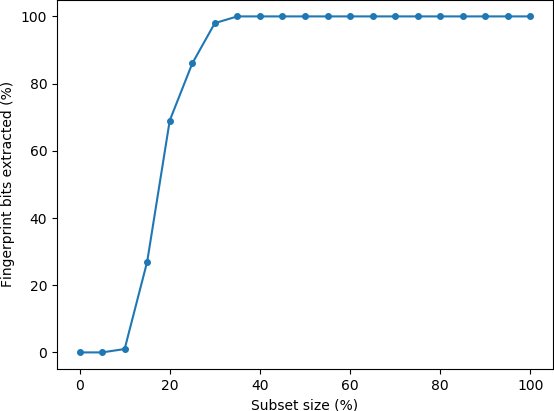
\includegraphics[width=6.7cm]{Figures/subset_attack_two-level_gamma100.png} }}
    \qquad
    \subfloat[$\gamma_1=50$]{{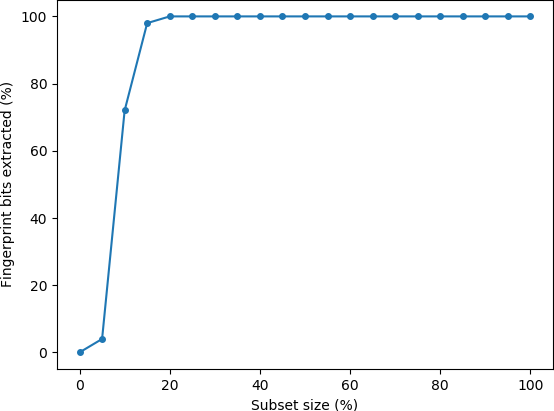
\includegraphics[width=6.7cm]{Figures/subset_attack_two-level_gamma50.png} }}
    \caption{Fingerprint extraction in a subset attack}
    \label{fig:subset-attack-two-level-fp-bits}
\end{figure}

The attack may cause that the extraction process does not manage to extract all the fingerprint bits correctly.
We can see from \Cref{fig:subset-attack-two-level-fp-bits}(a) that even if only around 35\% of the tuples are released by the malicious buyer, all fingerprint bits are still correctly extracted. 
The robustness of this scheme can be improved by changing the value of $\gamma_1$. 
\Cref{fig:subset-attack-two-level-fp-bits}(b) shows the results for a smaller $\gamma_1$, i.e. for the increased number of marks in the data that can be used to verify the ownership. 
For this parameter setting, the scheme is more robust against the subset attack, and even from only 20\% of the data, all the correct fingerprint bits can be extracted. 
For this experiments, we used the fingerprint of length $L=96$ and the bit significance level of each bit $\alpha_2$ is 0.01 (the confidence level is 99\%).

\begin{table}[ht]
    \centering
    \caption{Success of the subset attack on Two-level Fingerprinting Scheme}
    \label{tab:subset-attack-two-level}
    \begin{tabular}{|c|c|c|c|c|c|c|}
        \hline
         & $p'=60\%$ & $p'=70\%$ & $p'=80\%$ & $p'=90\%$ & $p'=95\%$ & $p'=99\%$ \\
         \hline
         $\gamma_1 = \gamma_2 = 10$ & 0 & 0 & 0 & 0 & 0 & 1.0 \\
         \hline
         $\gamma_1 = \gamma_2 = 25$ & 0 & 0 & 0 & 0.04 & 1.0 & 1.0 \\
         \hline
         $\gamma_1 = \gamma_2 = 50$ & 0 & 0 & 0.04 & 0.98 & 1.0 & 1.0 \\
         \hline
         $\gamma_1 = \gamma_2 = 100$ & 0 & 0.74 & 1.0 & 1.0 & 1.0 & 1.0 \\
         \hline
         $\gamma_1 = \gamma_2 = 200$ & 1.0 & 1.0 & 1.0 & 1.0 & 1.0 & 1.0 \\
         \hline
    \end{tabular}
\end{table}

Let us consider the setting where $\gamma_1=50$ and $\gamma_2=50$. For $p<20\%$ ($p'>80\%$; the attacker removes more than 80\% of the tuples) some bit positions will be unknown. For $p=15\%$ on average 2 out of 96 bit positions cannot be detected, creating $2^2$ fingerprint candidates. 
The fingerprint verification process may still select the correct fingerprint out of $2^2$ possible ones and the extraction algorithm finds the malicious buyer successfully. 
In the same setting, when 90\% of the tuples are removed, the algorithm correctly extracts 72\% correct fingerprint bits, or 69 out of 96. 
This is not enough for the fingerprint verification algorithm to verify any fingerprint and the detection algorithm fails. 
See the \Cref{tab:subset-attack-two-level} where the success of the subset attack is recorded. 
The experiments are run using Forest Cover Type data. 
The results in the table confirm that although not all fingerprint bits are extracted, the attack is not 100\% successful. 

\begin{figure}
    \centering
    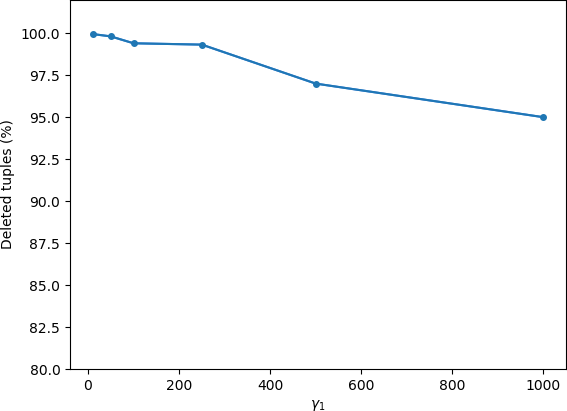
\includegraphics[width=0.7\textwidth]{Figures/subset_attack_two-level-ownership-ver.png}
    \caption{Ownership verification in a subset attack}
    \label{fig:subset-attack-ownership-verification}
\end{figure}

The first level of the embedding process provides the ownership verification even for cases when the correct fingerprint cannot be extracted. 
So, although the owner cannot trace the source of unauthorised leakage of data, she can claim the ownership. The mark created in this process is very robust. See in the \Cref{fig:subset-attack-ownership-verification} that even from the very small percentage of the data (<5\%), the detection algorithm will verify the owner with confidence level 99\% ($\alpha_1=0.01$).
The experiments are run even for the very big values of $\gamma_1$. 
For the settings where our experiments show high probabilities of extracting the right fingerprint from the small chunks of data, i.e $10<\gamma_1,\gamma_2<100$, up to 99\% of the tuples can be deleted and ownership can still be claimed.      

\subsection{Fingerprinting scheme for categorical data}
The fingerprinting scheme for categorical data complements the AK Scheme and for subset attack, we can refer to \Cref{eq:subset-attack-ak} as a starting point for analysis. 
The important difference between AK Scheme and scheme for categorical data is the introduction of modulo operation as one of the steps. 
We mentioned before in \Cref{subsec:fingerprinting-scheme-categorical} that we trade the strength of detection algorithm for fingerprinting categorical data successfully. 
This means that additional modulo operation step in the fingerprint insertion phase causes errors in the detection phase that cannot be avoided. 
Having errors in unaffected fingerprinting scheme increases the vulnerability of the scheme to attacks. 
Therefore, the \Cref{eq:subset-attack-ak} lacks influence of modulo operation in order to be credible. 
\Cref{tab:subset-attack-adult} shows the theoretical success of the subset attack on the dataset with $\eta = 30,162$ rows (convenient for comparison to experimental results on Adult dataset) if the effects of modulo are not taken into account, using \Cref{eq:subset-attack-ak}.
$\omega_i$ is approximated to $\eta/(\gamma*L)$ and $L=80$. 
Value 0 represents the perfect resistance to the subset attack, and 1 is the perfect success of the subset attack, i.e. the scheme completely failing to defend against it.

\begin{table}[ht]
    \centering
    \caption{Theoretical success rate of a subset attack on the fingerprinting scheme for categorical data, using the Adult data}
    \label{tab:subset-attack-adult}
    \begin{tabular}{|c|c|c|c|c|c|c|}
         \hline
        & \textbf{$p'=30\%$} & \textbf{$p'=60\%$} & \textbf{$p'=80\%$} & \textbf{$p'=90\%$} & \textbf{$p'=95\%$} & \textbf{$p'=99\%$}\\
        \hline
        $\gamma=3$ & 0.0 & 0.0 & 0.0 & 0.0001 & 0.1174 & 1.0 \\
        \hline
        $\gamma=6$ & 0.0 & 0.0 & 0.0001 & 0.0996 & 0.9601 & 1.0 \\
        \hline
        $\gamma=12$ & 0.0 & 0.0 & 0.0762 & 0.9555 & 1.0 & 1.0 \\
        \hline
        $\gamma=25$ & $1.15\times10^{-6}$ & 0.3166 & 0.9430 & 1.0 & 1.0 & 1.0 \\
        \hline
        $\gamma=50$ & 0.0052 & 0.7421 & 1.0 & 1.0 & 1.0 & 1.0 \\
         \hline
        $\gamma=100$ & 0.4783 & 0.9999 & 1.0 & 1.0 & 1.0 & 1.0 \\
         \hline
     \end{tabular}
\end{table}

\paragraph{Experiments}
The experiments are made on the Adult dataset as it is the dataset containing categorical attributes. 
We measure the success of subset attack over 500 runs and parameters set as follows: $L=80$, $\xi=1$, $\tau=0.5$, $\gamma=\{3,6,12,25,50,100\}$ and $p'=\{0.30,0.60,0.80,0.90,0.95,0.99\}$, where $p'$ represents the percentage of tuples that are deleted.


\begin{table}[ht]
    \centering
    \caption{Experimental results of the subset attack success rate on the fingerprinting scheme for categorical data, using the Adult data}
    \label{tab:subset-attack-adult-experimental}
    \begin{tabular}{|c|c|c|c|c|c|c|}
         \hline
        & \textbf{$p'=30\%$} & \textbf{$p'=60\%$} & \textbf{$p'=80\%$} & \textbf{$p'=90\%$} & \textbf{$p'=95\%$} & \textbf{$p'=99\%$}\\
        \hline
        $\gamma=3$ & 0.0 & 0.0 & 0.0 & 0.004 & 0.22 & 1.0 \\
        \hline
        $\gamma=6$ & 0.08 & 0.18 & 0.20 & 0.354 & 0.954 & 1.0\\
        \hline
        $\gamma=12$ & 0.078 & 0.0 & 0.212 & 0.97 & 1.0 & 1.0 \\
        \hline
        $\gamma=25$ & 0.012 & 0.284 & 0.99 & 1.0 & 1.0 & 1.0 \\
        \hline
        $\gamma=50$ & 0.346 & 1.0 & 1.0 & 1.0 & 1.0 & 1.0 \\
         \hline
        $\gamma=100$ & 0.976 & 1.0 & 1.0 & 1.0 & 1.0 & 1.0 \\
         \hline
     \end{tabular}
\end{table}

\Cref{tab:subset-attack-adult} and \Cref{tab:subset-attack-adult-experimental} share the same parameter settings for calculating the success of a subset attack on the Adult dataset, however, in latter the rate of success is larger overall.
Although the detection algorithm can detect the correct fingerprint from the full set of tuples, the errors introduced by modulo operation are enhancing the success of the attack. 
Therefore, only for small values of $\gamma$, the scheme is resistant to subset attack if the large portion of tuples is not deleted. 




\section{Superset attack}\label{subsec:superset-attack}

In a superset attack, an attacker adds additional tuples to the fingerprinted data, creating a bigger, pirated dataset.
This attack considers only the addition of the new tuples while the original set of tuples remains in the pirated dataset.
The sources of the additional tuples can be various.
One can add the tuples from other sources such as related datasets with similar attributes, artificial tuples with some semantic meaning, tuples generated from the dataset itself, or the values can be completely random. 
This attack can only be applied on fingerprinting schemes whose defence algorithms can and do function without the access to the original dataset (e.g. AK Scheme).
Otherwise, it is trivial to compare the pirated dataset to the original and remove the tuples that are added by an attacker.


Defence in some cases can be helped by syntactical examination of the dataset. 
In cases where additional tuples are generated completely randomly, it might be easy for a human to spot and remove them without any algorithm.
Also, any semantic background that the defence knows about the database can serve as the preliminary step in the deletion of additional tuples.


\subsection{AK Scheme}\label{subsec:superset-attack-ak}
Assume that fingerprint bit $f_i$ is embedded in the original data $\omega_i$ times, and that it is extracted from the additional tuples $\omega_i'$ times \cite{li2005fingerprinting}. 
Matching of the single extracted fingerprint bit to the correct value $f_i$ is modelled as an independent Bernoulli trial with probability 0.5 of success or failure.
(Extraction is controlled by the new unknown values of the primary key, therefore it is equally likely for the extracted bit to be 0 or 1.)
For the detection algorithm to fail in extracting the correct fingerprint bit, at least $(1-\tau)(\omega_i+\omega_i')$ embedded bits that correspond to the fingerprint bit $f_i$ must be detected wrongly.
Thus, the probability that the fingerprint is detected incorrectly is $B((1-\tau)(\omega_i+\omega_i');\omega_i',0.5)$.
The probability that the entire fingerprint is detected incorrectly is 
\begin{equation} \label{eq:superset-attack}
    fm = 1 - \prod_{i=0}^{L-1}(1-B((1-\tau)(\omega_i+\omega_i');\omega_i',0.5))
\end{equation}

Let us set $\tau=0.5$ (the usual default value) and analyse the performance of superset attack success for that case.
Knowing that all fingerprint bits will be correctly extracted from the original tuples because they are not changed, intuitively, in the tuples added by the attacker the incorrect occurrence of some fingerprint bit must outnumber its occurrences in the original tuples.
Formally, superset attack can be successful only if $\exists i\in\{0,...,L-1\}: \omega_i'\geq\omega_i$.
To make that possible, the attacker must add at least $100\%\eta$ tuples to the original data.

In AK Scheme the choice of fingerprint bit to be embedded is made randomly and independently in each step, therefore we can assume $\omega_i\approx\omega_j, \forall i,j \in \{0,...,L-1\}, i \neq j$. 
Furthermore, we can also assume $\omega_i'\approx\omega_j', \forall i,j \in \{0,...,L-1\}, i \neq j$.
\Cref{tab:superset-attack-forest} shows the success of the superset attack depending on $\gamma$ and number of added tuples. 
The success is calculated using \Cref{eq:superset-attack}, taking into account the assumptions made above. 
We analyse the success of superset attack for Forest Cover Type data with $L=96$ and $\tau=0.5$
Value 0 is the complete failure of the attack and 1 maximum success. 

\begin{table}[ht]
    \centering
    \caption{Superset attack success rate on the Forest Covertype data}
    \label{tab:superset-attack-forest}
    \begin{tabular}{|c||c|c|c|}
    \hline
         $\omega_i'$ & $\gamma=25$ & $\gamma=50$ & $\gamma=100$ \\
        \hline
         $100\%(\omega_i)$ & $1.35835\times10^{-71}$ & $3.61112\times10^{-35}$ & $8.32668\times10^{-17}$ \\
         \hline
         $200\%(\omega_i)$ & $1.91325\times10^{-27}$ & $8.66310\times10^{-14}$ & $1.81092\times10^{-6}$ \\
         \hline
         $300\%(\omega_i)$ & $8.32595\times10^{-18}$ & $9.89990\times10^{-9}$ & $0.000439$ \\
         \hline
         $400\%(\omega_i)$ & $3.31239\times10^{-13}$ & $1.55168\times10^{-6}$ & 0.006221 \\
         \hline
         $500\%(\omega_i)$ & $1.74078\times10^{-10}$ & 0.000047 & 0.029978 \\
         \hline
         $1000\%(\omega_i)$ & 0.000045 & 0.019113 & 0.536146 \\
         \hline
    \end{tabular}
\end{table}

The ratio $\omega_i/\omega_i'$ is approximately the same as ratio $\eta/\eta'$, where $\eta'$ is the number of added tuples because of the randomness in embedding the fingerprint, so we can interpret the percentages in the first row of \Cref{tab:superset-attack-forest} as the amount of added tuples in with respect to the original number of tuples. 

The success rates in the \Cref{tab:superset-attack-forest} are very small even for cases with a big number of added tuples, i.e. the scheme is very resilient to superset attack. 
Adding a lot of "fake" tuples to the dataset, in this case even several times more than the original dataset size, violates the credibility of the data. 
The attacker does not benefit from such attack, so the subset attack is usually combined with some other attack such as subset attack (\textit{mix-and-match} attack \cite{li2005fingerprinting}). 

\paragraph{}
Superset attack requires the generation of new "fake" rows which can be achieved in several ways. 
The attacker might come up with brand new values and combine them into new tuples or use the existing ones. 
In any case, the semantic problem might arise if the new values, or a combination of them, do not contextually fit the attribute or the dataset. 
For example, assume we have a dataset with information about persons such as their age, weight, height, etc. 
Generating new tuples might result in having tuples with illogical values for attributes, for example \textit{height}:240cm or a same person with values \textit{age}:10y. and \textit{height}:190cm.
In this case, the defence against the attack might be trivial, only by removing such tuples from the pirated dataset. 

One possible superset attack model consists of generating new tuples from the existing fingerprinted data and mixing those with the original fingerprinted data to create a pirated dataset.
The tuples are generated such that every attribute value (except for the private key) is independently randomly chosen from the set of existing values for that attribute.
This way we make it harder for a human to distinguish between the tuples originating from the originally fingerprinted data and those added by the attacker, making the defence rely entirely on detection algorithm.
The example of tuple generation is shown in \Cref{table:superset-attack-tuple-gen}.
The original tuples from which the values are generated are singled out and the sampled values are highlighted.
In the last row, we can see the generated tuple.


\begin{table}[ht]
\centering
\caption{Example of tuple generation}
\label{table:superset-attack-tuple-gen}
\resizebox{\textwidth}{!}{
\renewcommand{\arraystretch}{1.4}
\begin{tabular}{|c|c|c|c|c|c|c|c|c|c|c|c|} 
 \hline
 Id & El. & Asp. & Slope & HD-H & VD-H & HD-R & HS-9am & HS-noon & HS-3pm & HD-FP & C-Type\\
 \hline
 75 & 2864 & 118 & 18 & \textbf{\Large{201}} & 74 & 4567 & 248 & 221 & 93 & 4849 & \textbf{\Large{2}} \\
 \hline
 191 & 2995 & 173 & 15 & 268 & \textbf{\Large{135}} & 6312 & 228 & 246 & 146 & 4135 & \textbf{\Large{2}}\\
 \hline
 893 & 2924 & 270 & 10 & 134 & 11 & 5066 & 194 & 244 & \textbf{\Large{189}} & 1652 & 5\\
 \hline
 1258 & 2803 & \textbf{\Large{57}} & 32 & 323 & 136 & 342 & 223 & 157 & 45 & 1851 & 5\\
 \hline
 2165 & \textbf{\Large{3390}} & 59 & 10 & 124 & 12 & 2610 & 228 & 219 & 124 & 2357 & 7\\
 \hline
 6880 & 2983 & 297 & \textbf{\Large{11}} & 713 & -51 & 1543 & 190 & 237 & 186 & \textbf{\Large{2003}} & \textbf{\Large{2}}\\
 \hline
 11643 & 2911 & 332 & \textbf{\Large{11}} & 67 & 2 & 4972 & 193 & 225 & 172 & 1724 & 5\\
 \hline
 19210 & 2737 & 20 & 7 & 95 & 14 & \textbf{\Large{2314}} & 215 & 225 & 147 & 6815 & \textbf{\Large{2}}\\
 \hline
 23117 & 2877 & 165 & 3 & 30 & 4 & 5236 & \textbf{\Large{222}} & 240 & 154 & 4279 & 1\\
 \hline
 23135 & 2801 & 116 & 9 & 30 & 2 & 4709 & 236 & \textbf{\Large{231}} & 126 & 4807 & \textbf{\Large{2}}\\
 \hline
 \hline
 \large{581012} & \large{3390} & \large{57} & \large{11} & \large{201} & \large{135} & \large{2314} & \large{222} & \large{231} & \large{189} & \large{2003} & \large{2}\\
 \hline
\end{tabular}}
\end{table}

\subsection{Block Scheme}
Superset attack essentially does not work if the original dataset is available in the fingerprint detection process. 
Block Scheme detection algorithm requires the original dataset to extract the fingerprint as discussed in \Cref{subsec:block-oriented-scheme}, therefore this kind of attack alone, without a combination with some other attack does not make much sense.
The owner trivially removes the tuples from the pirated dataset that are not part of the original and proceeds with the detection algorithm.

\subsection{Fingerprinting scheme for the categorical data}
The blind, simplistic fingerprinting scheme described in \Cref{subsec:fingerprinting-scheme-categorical} behaves in the same way as the AK Scheme against the superset attack. Therefore, we refer to \Cref{subsec:superset-attack-ak}.

The second discussed scheme which is based on neighbourhood search is not blind. It means that any additional fake tuples in the dataset would easily be detectable and removed by a simple check and comparison with the original dataset.

\section{Bit-flipping attack}
The subset and superset attacks described in \Cref{subsec:subset-attack} and \Cref{subsec:superset-attack} respectively, are targeting the disruption of tuples without changing the values inside the dataset. 
However, the attacker might change values by selecting some bits and flipping their values in an attempt to destroy the fingerprint.
This kind of attack is called a bit-flipping attack.
The choice of the bits is random because the attacker is modelled such that he has no knowledge about the owner's secret key that is crucial for fingerprint insertion scheme.

\subsection{AK Scheme}
Let \textit{p} be the probability that the attacker flips some $k^{\text{th}}$ least significant bit, with $p \leq 0.5$ (otherwise fingerprint detection can be applied to transformed data by flipping each fingerprintable bit back). 
The attacker chooses bits independently, therefore bit flipping is modelled as an independent Bernoulli trial with probability \text{p} of success and $1-p$ of failure. 
Assume that each fingerprint bit $f_i$ is embedded $\omega_i$ times.
The detection algorithm will fail to extract the correct fingerprint bit if the correct bit value is extracted less than the defined number of times which is controlled by parameter $\tau$.
Therefore at least $(1-\tau)\omega_i$ embedded bits must be flipped by an attacker.
Thus, the probability that the fingerprint $f$ is detected incorrectly is
\begin{equation}\label{eq:fm-bit-flipping-ak}
    fm=1-\prod_{i=0}^{L-1}(1-B(\lfloor(1-\tau)\omega_i\rfloor;\omega_i,p))
\end{equation}

Because the choice of fingerprint bits to be embedded in fingerprint embedding process is completely random, we can assume that each fingerprint bit will be embedded in the data approximately same number of times; $\omega_0=\omega_1=...=\omega_{L-1}=\omega, \forall i, j \in \{1,L-1\}, i\neq j$.
Therefore, we can write the expression for false miss rate (\Cref{eq:fm-bit-flipping-ak}) as $fm = 1 - (1-B(\lfloor(1-\tau)\omega\rfloor;\omega,p))^L$.
The results in \Cref{table:bit-flipping-ak} and \Cref{table:bit-flipping-ak-tau} are obtained using this approximation of false miss rate. 
Since $0<B(\lfloor(1-\tau)\omega\rfloor;\omega,p)\leq1$, by increasing $L$ the false miss rate also increases, meaning that longer fingerprints lead to schemes more vulnerable to bit-flipping attack.
Intuitively, longer fingerprint means fewer embeddings of each single fingerprint bit in the data and larger probability for the attacker to erase all of the embeddings of some fingerprint bit, making the detection algorithm incapable of detecting a valid fingerprint. 

The effect of parameter $\gamma$ is shown in \Cref{table:bit-flipping-ak} by calculating probabilities of success of bit-flipping attack for different values of $\gamma$ and $p$ (probability of flipping a bit, i.e. the approximate amount of tuples containing a value with a flipped bit).
We choose $\gamma=\{6, 12, 25, 50, 100, 200\}$ and $p=\{45\%, 40\%, 30\%, 20\%\}$, and set $\tau=0.5$ and $L=96$ as fixed values.
$\omega$ is calculated as $\eta/(L*\gamma)$, and $\eta=581,012$ for the convenience of comparing these results to the experimental results on Forest Covertype dataset.

\begin{table}[ht]
\centering

\caption{Probability of a successful bit-flipping attack on the AK Scheme}
\label{table:bit-flipping-ak}
\begin{tabular}{|c|c|c|c|c|} 
 \hline
   & \textbf{$p=20\%$} & \textbf{$p=30\%$} & \textbf{$p=40\%$} & \textbf{$p=45\%$} \\
 \hline
 $\gamma=6$ & 0 & 0 & $6.6530 \times 10^{-9}$ & 0.0671 \\
 \hline
 $\gamma=12$ & 0 & 0 & 0.0003 & 0.7327 \\
 \hline
 $\gamma=25$ & 0 & $5.8392\times 10^{-9}$ & 0.0941 & 0.9987 \\
 \hline
 $\gamma=50$ & 0 & 0.0002 & 0.7144 & 1 \\
 \hline
  $\gamma=100$ & $2\times 10^{-5}$ & 0.0839 & 0.9994 & 1 \\
  \hline
  $\gamma=200$ & 0.0220 & 0.8060 & 1 & 1 \\
 \hline
\end{tabular}
\end{table}

The effect of parameter $\tau$ is shown in \Cref{table:bit-flipping-ak-tau}.
The success of the bit-flipping attack is calculated for different values of $\tau$ and $p$, while $L=96$ and $\gamma=50$ are set as fixed values.

\begin{table}[ht]
\centering
\caption{Probability of a successful bit-flipping attack on the AK Scheme}
\label{table:bit-flipping-ak-tau}
\begin{tabular}{|c|c|c|c|c|} 
 \hline
 & \textbf{$p=45\%$} & \textbf{$p=40\%$} & \textbf{$p=30\%$} & \textbf{$p=20\%$} \\
 \hline
 $\tau=0.50$ & 1 & 0.7144 & 0.0002 & 0 \\
 \hline
 $\tau=0.55$ & 1 & 0.9999 & 0.0228 & 0 \\
 \hline
 $\tau=0.60$ & 1 & 1 & 0.5779 & $2\times 10^{-5}$ \\
 \hline
 $\tau=0.65$ & 1 & 1 & 1 & 0.0048 \\
 \hline
  $\tau=0.70$ & 1 & 1 & 1 & 0.3041 \\
  \hline
  $\tau=0.75$ & 1 & 1 & 1 & 0.9996 \\
 \hline
\end{tabular}
\end{table}

Both $\tau$ and $\gamma$ affect the success of the attack such that if they are increased, the probability that fingerprint will not be detected correctly is also increased, i.e. the scheme is more susceptible to bit-flipping attack.
Generally, if the attacker chooses to flip more bits, i.e. increases $p$, that also increases his chance for the successful attack, but in the same time violates credibility of the data since more original values would be changed.
Note that parameter $\xi$ does not affect the success of the attack because it is not important which LSB of a chosen value is flipped by the attacker. 

\paragraph{Misattribution false hit}
Let us now analyse the probability of detecting valid but incorrect fingerprint caused by a bit-flipping attack - misattribution false hit $fh^A$.
The detection algorithm will extract a binary bit for fingerprinting bit $f_i$ if either at most $\lfloor(1-\tau)\omega_i\rfloor-1$ or at least $\lfloor\tau\omega_i\rfloor$ of its embedded bits are flipped.
If the detection algorithm extracts a binary string, the probability that the binary string is valid but belongs to an innocent buyer is $\frac{N-1}{2^L}$.
Therefore, the probability of detecting valid but incorrect fingerprint is 
\begin{equation} \label{missattribution-false-hit-ak-bit-flipping}
    fh^A=\frac{N-1}{2^L}\prod_{i=0}^{L-1}(1-B(\lfloor(1-\tau)\omega_i\rfloor;\omega_i,p)+B(\lfloor\tau\omega_i\rfloor;\omega_i;p)).
\end{equation}

\paragraph{}
False miss rate is by definition the sum of misattribution false hit and false negative rate.
Therefore, false negative is straightforward:

\begin{equation}
\begin{aligned}
fn=& 1-\prod_{i=0}^{L-1}(1-B(\lfloor(1-\tau)\omega_i\rfloor;\omega_i,p))- \\ & \frac{N-1}{2^L}\prod_{i=0}^{L-1}(1-B(\lfloor(1-\tau)\omega_i\rfloor;\omega_i,p)+B(\lfloor\tau\omega_i\rfloor;\omega_i;p)).
\end{aligned}
\end{equation}

\paragraph{Experiments}
We have run experiments on the Forest dataset and obtained results that are shown in table \ref{table:bit-flipping-ak-emp}. 
As it is shown in the previous section, the success of bit-flipping attack is influenced by multiple parameters - length of the fingerprint \textit{L}, fingerprint detection assurance parameter $\tau$, amount of marked values $\gamma$ (or equivalently, number of embedded bits corresponding to a single bit $\omega$) and the attacker's parameter \textit{p} that defines the number of flipped bits in pirated data. 
For our experiments we fix the values of $L=96$ and $\tau=0.5$.
We run 100 experiments with different random bit-flipping pattern for each of the combinations of parameters $\gamma = {6,12,25,50,100}$ and $p={20\%,30\%,40\%,45\%}$.

\begin{table}[ht]
\centering
\caption{Experimental results of a bit-flipping attack on the AK Scheme, using the Forest Cover Type data}
\begin{tabular}{|c|c|c|c|c|} 
 \hline
 & \textbf{$p=20\%$} & \textbf{$p=30\%$} & \textbf{$p=40\%$} & \textbf{$p=45\%$} \\
 \hline
 $\gamma=6$ & 0 & 0 & 0.50 & 0.56  \\
 \hline
 $\gamma=12$ & 0  & 0 & 0.50 & 1.0 \\ 
 \hline
 $\gamma=25$ & 0  & 0 & 0.54 & 1.0  \\
 \hline
 $\gamma=50$ & 0 & 0.50 & 0.72 & 1.0   \\
 \hline
  $\gamma=100$ & 0 & 0.86 & 1.0 & 1.0  \\
 \hline
\end{tabular}
\label{table:bit-flipping-ak-emp}
\end{table}

The experimental results show that flipping 40\% of the bits available for fingerprinting most likely deletes the fingerprint. At 30\% the schemes with bigger $\gamma$ ($\gamma=50,100)$, i.e. less embedded marks, fail under the bit-flipping attack. 
Generally, the scheme is more robust against the attack for a smaller value of $\gamma$.
The empirical results differ from the analytic results in \Cref{table:bit-flipping-ak}. The two analysis agree on the cases where the attack completely succeeds and completely fails, however, in our experiments the scheme appears less robust to the bit-flipping attack than it is suggested in the analysis. 
The success rates in \Cref{table:bit-flipping-ak} are calculated using \Cref{eq:fm-bit-flipping-ak} under the assumption that all fingerprint bits are embedded the same number of times, which is approximated with $\omega$. 
This is not true due to the random nature of bit choice. In reality, every fingerprint bit has it's own $\omega_i$ value. Many fingerprint bits, thus, are embedded in data less than $\omega$ times and are easier to destroy. Since destroying all occurrences of just one fingerprint bit makes the fingerprint impossible to extract, the low occurrences of some fingerprint bits might decrease the robustness. 
This might be the reason for the difference in the attack success rates. 
Even though the probabilities for attack success are different, the boundary for robustness is confirmed. 
For $\gamma=\{6,12,25\}$ it is safe to flip up to 30\% of LSBs to not remove the fingerprint, and for larger values, $\gamma=\{50,100\}$, it is safe to flip around 20\% of the LSBs.

\subsection{Block Scheme}
Assume that the attacker examines every bit available for fingerprinting independently and selects it for flipping with probability $p$.
Let us approximate the number of times that each fingerprint bit is embedded in the data to $\omega$.
For the detection algorithm to fail to recover the correct fingerprint bit, at least $(1-\tau)\omega$ embedded bits corresponding to the single fingerprint bit $f_i$ must be changed, i.e. more than $\omega - \lceil\tau\omega\rceil+1$ bits must be changed.
Probability that one fingerprint bit is destroyed is $B(\omega-\lceil\tau\omega\rceil+1;\omega,p)$.
The probability that the entire fingerprint will be detected incorrectly is therefore 
\begin{equation}
    fm=1-(1-B(\omega-\lceil\tau\omega\rceil+1;\omega,p))^L
\end{equation}

Table \ref{table:bit-flipping-block} shows the probabilities that the bit-flipping attack will be successful on Block Scheme, depending on $p$ and $\beta$.
Parameters are set as follows: $\xi=2$, $\tau=0.5$ and $L=96$.
We choose $\eta=581012$ and $v=10$, same as Forest Covertype dataset. 

\begin{table}[ht]
    \centering
    \caption{Probability of a successful bit-flipping attack on the Block Scheme}
    \label{table:bit-flipping-block}
    \begin{tabular}{|c|c|c|c|c|}
    \hline
         & p=30\% & p=40\% & p=45\% & p=50\%\\
         \hline
        $\beta=5$ & 0 & 0 & 0 & 1.0 \\
        \hline
        $\beta=10$ & 0 & 0 & 0.02 & 1.0 \\
        \hline
        $\beta=15$ & 0 & 0.002 & 0.88 & 1.0 \\
        \hline
        $\beta=20$ & 0 & 0.017 & 0.97 & 1.0 \\
        \hline
    \end{tabular}
\end{table}


\paragraph{Experiments}
We run experiments on the Forest dataset with the previously defined parameters.
Table \ref{table:bit-flipping-block-emp} shows the obtained empirical results for the success of the bit-flipping attack on the Block Scheme.
Each experiment is run 100 times and the table shows the average success of the bit-flipping attack. 

\begin{table}[ht]
    \centering
    \caption{Experimental results of the bit-flipping attack on the Block Scheme, for the Forest Cover Type data}
    \begin{tabular}{|c|c|c|c|c|}
    \hline
         & p=30\% & p=40\% & p=45\% & p=50\%\\
         \hline
        $\beta=5$ & 0 & 0 & 0.50 & 1.0 \\
        \hline
        $\beta=10$ & 0 & 0.50 & 0.50 & 1.0 \\
        \hline
    $\beta=15$ & 0 & 0.50 & 0.92 & 1.0 \\
        \hline
        $\beta=20$ & 0.08 & 0.50 & 1.0 & 1.0 \\
        \hline
    \end{tabular}
    \label{table:bit-flipping-block-emp}
\end{table}

The experiments confirm the rule that having more marks in the data, i.e. smaller $\beta$, makes the scheme more robust against the bit-flipping attack.
Our experimental rates of the attack success, however, differ from the analytical results in \Cref{table:bit-flipping-block}. 
The change might be due to the implementation limitations introduced by the design of the Block Scheme. 
We address in \Cref{subsec:assumptions-block} the problem of "extra data" that in reality never gets fingerprinted.
This means that less data is fingerprinted, i.e. fewer marks are in the data due to this limitation than it is assumed for the calculation of the theoretical attack success rates.
This might be the reason why experimentally this scheme appears to be more vulnerable to the attack than expected by the theoretical analysis.

The scheme with all of the chosen parameters guarantees robustness for to 30\% flipped LSBs. Choosing a small value of $\beta$, e.g. 5, the tolerated amount of flipped bits rises up to 45\%.
We can argue that this is indeed a robust scheme. The assumed attacker would like to keep the data useful, and flipping more bits significantly changes the values in the data and the utility decreases.


\subsection{Two-level Fingerprinting Scheme}
In this section, we empirically analyse the robustness of the Two-level Fingerprinting Scheme against the bit-flipping attack. 
We measure the success on two levels; the ownership verification and the fingerprint extraction.
The attacker might be able to either (i) disable both ownership verification and fingerprint extraction, (ii) destroy the fingerprint but fail in disabling ownership verification, or (iii) fail in both. 
We use the Forest Covertype data for the experiments and measure success of the subset attack over 500 runs of each parameter setting. We choose: $L=96$, $\xi=2$, $\alpha_1=\alpha_2=\alpha_3=0.01$, $\gamma_1=\gamma_2=\{10,25,50,100\}$.
\Cref{fig:bit-flip-two-level-fp} shows the results of the experiments.

\begin{figure}[ht]
    \centering
    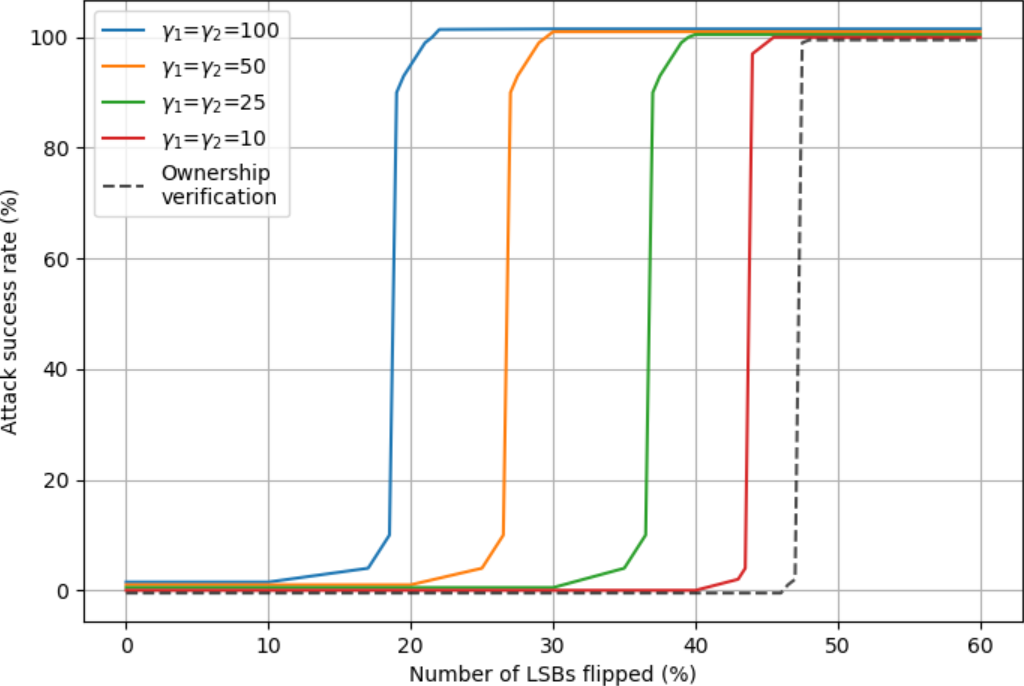
\includegraphics[width=0.9\textwidth]{Figures/bit-flip-two-level-screensh.png}
    \caption{Bit-flipping attack success in the Two-level Fingerprinting Scheme}
    \label{fig:bit-flip-two-level-fp}
\end{figure}

The coloured lines show the success rate of the attacks against the fingerprint extraction. 
The dashed line shows the success rate of the attack against the ownership verification.
The experiments show that the robustness against the bit-flipping attack, as expected, grows with more embedded marks.
The scheme with $\gamma_1=\gamma_2=100$ fails to extract the fingerprint when 19\% of the LSBs are flipped by the attacker, while the scheme with $\gamma_1=\gamma_2=10$ fails at approximately 43\% flipped LSBs.
In both cases, the ownership is verified 100\% of the times, even though the exact fingerprint cannot be extracted. 
The ownership verification fails with approximately 47\% flipped LSBs. 
The robustness of the ownership verification is very similar for each $\gamma_1$ value, therefore we represent it with only one (dashed black) line in \Cref{fig:bit-flip-two-level-fp}.

Choosing smaller $\gamma$ values makes the Two-level Fingerprinting Scheme very robust against the bit-flipping attack. The two-level fingerprint provides the additional protection measure of verifying the ownership even in cases when the exact fingerprint cannot be extracted. 
Smaller values of $\gamma$, however, introduce more error in data. How these errors affect the utility of the data, we discuss in \Cref{chapter:Utility}.

\section{Additive Attack}
Consider a scenario where the attacker tries to claim the ownership of the dataset by inserting an additional fingerprint in the bought dataset. We call this strategy an additive attack \cite{agrawal2003watermarking}. The competing ownership claims can be resolved if there exists at least one bit that both the owner and the attacker have marked, each with a different value. The way to resolve the ownership claim competition is to determine which owner's marks win, i.e. which mark has overwritten the other. The winning owner's mark is clearly inserted later, therefore his claim of ownership is false.

Method for dealing with the false claims of ownership could be to ask both the owner and the attacker to produce the original dataset before it was fingerprinted and to demonstrate the presence of the fingerprint in each other's original datasets. 
The owner will be able to demonstrate the presence of her fingerprint in the attacker's original unlike the attacker in the owner's original. 


\subsection{AK Scheme}\label{subsubsec:additive-ak}
In the AK Scheme, it is justified to conclude that the odds of finding such conflicting bits are low. 
Suppose that the data fingerprinted by the owner is marked $\omega$ times with parameters $\gamma$, $v$ and $\xi$ and that the attacker performs the fingerprinting insertion algorithm with parameters $\gamma'$, $v'$ and $\xi'$. Under the usual probabilistic model of AK Scheme's bit-marking process, the probability that a specified bit marked by original fingerprint is also marked by the attacker is the product of probabilities that the tuple containing the bit is chosen for marking $(1/\gamma')$, that the attribute containing the bit is also chosen for marking $(1/v')$ and that the specified bit is chosen $(1/\xi')$. The probability that the attacker's mark is different from the original mark is 1/2 so that the overall probability that the specified bit is a conflict bit is $1/(2\gamma'v'\xi')$. The tuples are marked independently of each other, therefore the probability that the attack is successful, i.e. no conflicting bits are found, is
\begin{equation}
    P\{success|\omega\}=(1-\frac{1}{2\gamma'v'\xi'})^\omega
\end{equation}

For example, let the dataset have around 500,000 tuples and  $\omega=1000$. 
Assume that attacker wants to increase his chances of success.
If the attacker sets $\gamma'=10,000$ (a rather big value considering that it means that only 1/10,000 tuples will be marked), $v'=10$ and $\xi'=5$, then $P\{success|\omega\}=(1-10^{-6})^1000 \approx 0.999$.



\subsection{Block Scheme}
The solution from section \ref{subsubsec:additive-ak} is applicable to the block fingerprinting scheme as well. 
Suppose that the attacker runs the fingerprint insertion algorithm with parameters $\beta'$, $\xi'$ and $v'$.  
Let $1/\gamma'$ be the percentage of tuples marked by the attacker.
Due to the uniform distribution of the marks in the Block Scheme, we can approximate the percentage $1/\gamma \approx (\xi v)/\beta^2$, assuming that there is in average no more than 1 mark in a single tuple.
Let the data be marked $L\omega$ times in total by the owner.
The probability that the additive attack is successful is then 

\begin{equation}
\begin{aligned}
    P\{success|L\omega\}&=(1-\frac{1}{2\gamma'v'\xi'})^{L\omega} \\
        &=(1-\frac{1}{2\frac{\beta'^2}{\xi'v'}v'\xi'})^{L\omega} \\
        &=(1-\frac{1}{2\beta'^2})^{L\omega}
\end{aligned}
\end{equation}

The success of the additive attack depends exponentially on $L\omega$.
The attacker can increase his chances for success by increasing $\beta'$, however with $L\omega \gg \beta'$, the chances for the successful attack are low.
For example, with $\beta'=30$ and $L\omega=10000$, $P\{success|L\omega\}=0.0039$.



\section{Collusion Attack} \label{subsec:collusion}

Fingerprinting produces distinct copies of the data for each of the buyers. 
This opens the possibility for multiple buyers to have access to each other's copies of the data, all fingerprinted with different fingerprints, and work in coalition in order to create a useful data copy that would not implicate any member of the coalition. 
One possibility for the members of the coalition is to attempt to erase the fingerprint or to modify values such that detection algorithm implies an innocent buyer who is not a member of the coalition to be the traitor.
Collusion attack is specific for fingerprinting, as opposed to other attacks discussed in this thesis that can be applied in the context of watermarking. 
Collusion is studied extensively in the literature \cite{boneh1998collusion, guth1999error, pfitzmann1999coin, pfitzmann1996asymmetric, yacobi2001improved} and collusion resistant fingerprinting codes have been proposed such as one by Blakley et al. \cite{blakley1985fingerprinting}, by Guth and Pfitzmann \cite{blakley1985fingerprinting}, and probably the most well-know by Boneh and Shaw - \textit{BoSh} \cite{boneh1998collusion}.

Boneh and Shaw \cite{boneh1998collusion} provide the definitions of collusion-secure codes and propose the methods for construction of codes and algorithm for dealing with collusion attacks. 
The method can be used for fingerprinting any sort of digital data: documents, multimedia, software, etc. 
The effectiveness of the approach is based on the \textit{Marking Assumption} that states that "the main property of the marks should be satisfied are that users cannot change the state of an undetected mark without rendering the object useless" \cite{boneh1998collusion}. The colluding buyers can detect only the fingerprint bits in which their copies differ, otherwise, the fingerprint cannot be detected. 
For instance, two buyers with their fingerprinted dataset can fairly easily compare their datasets and remove or change the values that differ between the copies.

The following definitions of collusion-secure codes are defined \cite{boneh1998collusion}:
\begin{itemize}
    \item \textbf{$c$-frameproof code} satisfy that no coalition of at most \textit{c} members can frame a user who is not part of the coalition. $c$-frameproof codes prevent this harder version of treason but do not assure that the traitor(s) will be found
    
    \item \textbf{totally $c$-secure code} is a code for which exist an algorithm that outputs a member of a coalition with at most $c$ members that generated an arbitrary code under the coalition. It is proven that for $c \geq 2$ the totally c-secure code does not exist.
    
    \item \textbf{$c$-secure code with $\epsilon$-error} is a relaxation of the previous - if the code is $c$-secure with $\epsilon$-error, then there exists an algorithm which outputs a member of coalition with at most $c$ members with probability $1-\epsilon$, $\epsilon \in [0,1]$. 
\end{itemize}

BoSh codes are designed to be $c$-secure with $\epsilon$-error. 
Increasing $c$ or reducing $\epsilon$ provides better security definition, but results in longer codes.
BoSh code is generated as a concatenation of $b$ code-words of size $(a-1)d$ from public "inner code" that is common for all buyers. 
Therefore, the code has length $b(a-1)d$.
Code words from the inner code are chosen according to the secret buyer-specific "outer code" and randomly permuted before the use. 
$a$, $b$ and $d$ are code construction parameters (in \cite{boneh1998collusion} $n$, $L$ and $d$ respectively, but we change the notation due to overlapping with notation in this thesis).
The parameter values are: $a=2c$, $b=2c\log(2N/\epsilon)$ and $d=2a^2 \log(4ab/\epsilon)$.
It is required that the random permutation and random outer code for each buyer are kept secret from all buyers.
The tracing algorithm takes as input pirated data under collusion attack and returns exactly one malicious buyer. 

\paragraph{AK Scheme}
AK insertion algorithm (\Cref{alg:AK-insertion}) is not secure against collusion attack. 
Each fingerprint bit $f_i$ is embedded to the same place in every fingerprinted copy of the dataset since it only depends on parameters $\gamma$, $v$ and $\xi$ which are not buyer-specific, and owner's secret key $\mathcal{K}$.
Assume that 3 buyers are in collusion and they extract following marks from the bits that differ within their copies: (1,0,1), (1,1,0) and (0,1,1). 
They decide to change values according to the majority, so they come up with the new mark (1,1,1) that they use to create the pirated data. 
Detection algorithm cannot match the new fingerprint to any of the members of the coalition. 
Another option for members of the collusion is to produce a random mark, e.g. (0,0,1) which leads to the same outcome. 

To create a collusion-resistant scheme, authors in \cite{li2005fingerprinting} propose the modified version of BoSh code that is adequate to be incorporated into AK Scheme. 
The fingerprint in the proposed solution consists of two parts: (1) watermark which is the same for every buyer and computed from a hash function using owner's secret key, $\mathcal{H}(\mathcal{K})$, and (2) BoSh code. 
Those two parts are concatenated to create the fingerprint.

There are two main differences between BoSh code and proposed solution \cite{li2005fingerprinting}:
\begin{enumerate}
    \item Collusion-resistant AK Scheme does not require recording of secret outer code for every buyer as it is the case for BoSh codes. Storing any kind of secret buyer-specific information is already discussed to violate key-based property and as a reason for incorporating pseudo-random sequence generator in the context of a fingerprint. The outer code needs to be hidden from the buyers, but deterministic to the owner. Therefore, the outer code is in collusion-resistant AK Scheme generated using such pseudo-random sequence generator from the owner's secret key $\mathcal{K}$ and buyer's ID number.
    
    \item Similarly, the random permutation for all buyers needs to be stored in BoSh code setting. The purpose of the final random permutation in BoSh code is to hide which mark in dataset corresponds to which fingerprint bit. In AK Scheme this permutation is not necessary as the choice of fingerprint bit to be embedded is already random by the design of the insertion algorithm (lines 7 and 8 in \Cref{alg:AK-insertion}).
    
\end{enumerate}

Insertion and detection algorithms of collusion-resistant AK Scheme are slightly modified insertion (\Cref{alg:AK-insertion}) and detection (\Cref{alg:AK-detection}) algorithms of AK. 
The modifications in the insertion algorithm are as follows:
\begin{enumerate}
    \item Additional parameter $L_1$ represents the length of the first (watermarking) part of a fingerprint. $L=L_1+L_2$ ($L_2$ is the length of second part - BoSh code).
    \item Generation of fingerprint replaced by concatenation of watermark part of the fingerprint and BoSh code.
    \item Additional parameter $c$ - maximum coalition size
    \item Additional parameter $\epsilon$ - maximum false detection rate in tracing a coalition
\end{enumerate}
The detection algorithm is modified such that it runs in two consecutive phases:
\begin{enumerate}
    \item \textbf{Watermark check} - in this part, the watermark part $\mathcal{F_1}$ of recovered fingerprint template $\mathcal{F}$ is checked against the inserted codeword. The algorithm returns \textit{none suspected} for a single bit mismatch. This phase serves as prevention from 100\% misdiagnosis false hit rate in cases where non-pirated data is the input of detection algorithm (because the following phase returns exactly one malicious buyer). 
    \item \textbf{BoSh tracing algorithm} (from \cite{boneh1998collusion}) - if algorithm passes the first phase, this phase identifies exactly one malicious buyer.
\end{enumerate}

Authors of \cite{li2005fingerprinting} analyse the robustness rates of collusion-resistant AK Scheme and carry out the experimental results on scheme robustness.
Following the proof from \cite{boneh1998collusion} that probability of BoSh tracing algorithm returning the buyer who is indeed a member of the coalition is greater than $1-\epsilon$, the false miss rate $fm$ and misattribution false hit $fh^A$ satisfy
\begin{equation}
    fm=fh^A \leq \epsilon
\end{equation}
The misdiagnosis false hit $fh^D$ when the detection algorithm is applied on unmarked dataset is
\begin{equation}
    fh^D=\prod_{i=0}^{L_1-1}B(\lfloor\tau\omega_i\rfloor;\omega_i,0.5)\leq \frac{1}{2^{L_1}})
\end{equation}
and it can be decreased exponentially by increasing $L_1$ ($fh^D \simeq0$ if $L_1 \gg 1$).


\section{Summary}
In this chapter, we analysed the robustness of the fingerprinting techniques under certain types of attacks. We address subset attack, superset attack, bit-flipping attack, additive attack and collusion attack. 
As opposed to analysing the inability of a scheme to detect the fingerprint under a malicious attack, we also address the possibility of detecting the fingerprint in unmarked data - misdiagnosis false hit.

%misdiagnosis
\begin{figure}[ht]{
    \centering
    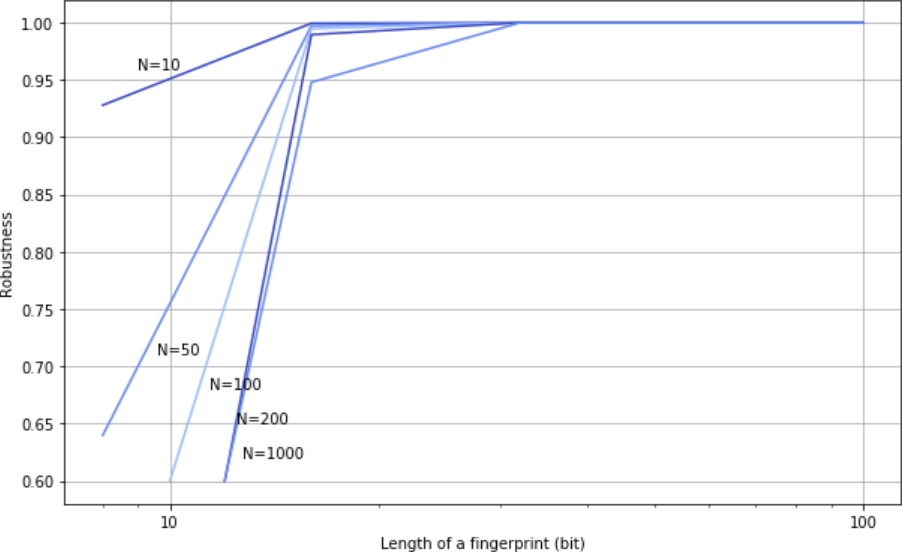
\includegraphics[width=0.8\textwidth]{Figures/misdiagnosis.PNG}
    \caption{Misdiagnosis false hit rate}
    \label{fig:misdiagnosis}
 }   
 \end{figure}

To avoid the misdiagnosis false hit, the fingerprint length must be big enough. \Cref{fig:misdiagnosis} shows the robustness of a scheme given the assumed number of buyers. We see that for the larger number of buyers we must ensure the longer fingerprint, e.g. if there are 100 buyers, the fingerprint length $L$ should be larger than 30.
 
The additive attack is, like misdiagnosis false hit, not specific for a certain scheme. The robustness of the scheme against the additive attack depends on the number of marks the scheme embeds in the data, which is controlled by parameters $\gamma$ in AK Scheme and the Scheme for fingerprinting categorical data, by $\gamma_1$ and $\gamma_2$ in Two-level Scheme and by $\beta$ in the Block Scheme.
%additive
\begin{figure}{
    \centering
    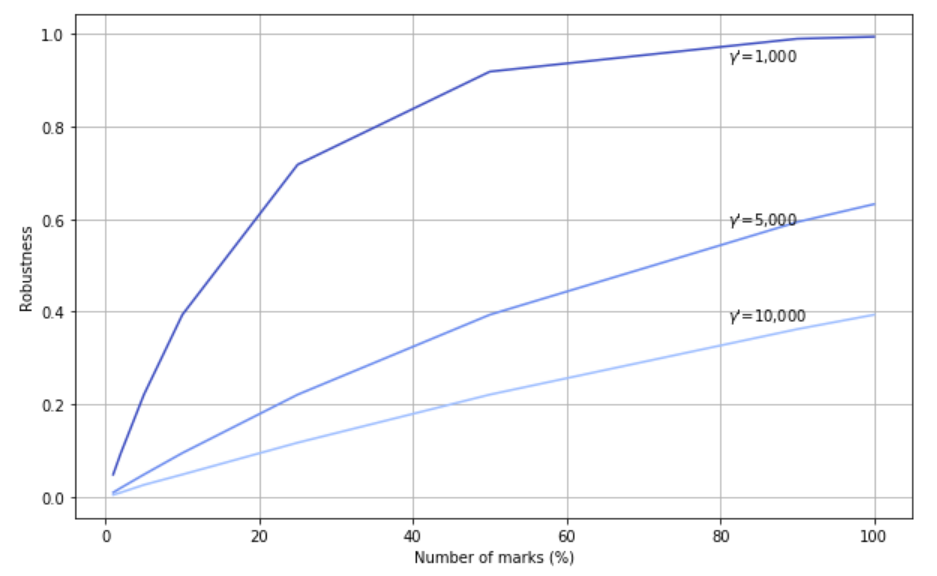
\includegraphics[width=0.8\textwidth]{Figures/additive.PNG}
    \caption{Robustness against the additive attack}
    \label{fig:additive-attack}
}\end{figure}
%subset
We show in \Cref{fig:additive-attack} the relation between number of marks and robustness of the scheme for different attacker's embedding patterns. 
The attacker's parameter of the ratio of the marked tuples is $\gamma'$ ($\gamma'=1,000$ means that one in a thousand tuples is marked). 
It depends on the attacker how he chooses to embed his fake fingerprint. If the dataset is very big and marking one in 10,000 tuples is sufficient to claim his ownership, then the fingerprinting schemes are not very robust - there is only 40\% chance that the attacker will not succeed. However, smaller datasets (10,000 tuples or less) might be harder to attack since the attacker would need to choose smaller $\gamma'$ to be able to claim the ownership. Schemes are much more robust if the attacker chooses $\gamma'<1,000$.

\begin{figure}
    \centering
    \begin{minipage}{0.49\textwidth}{
        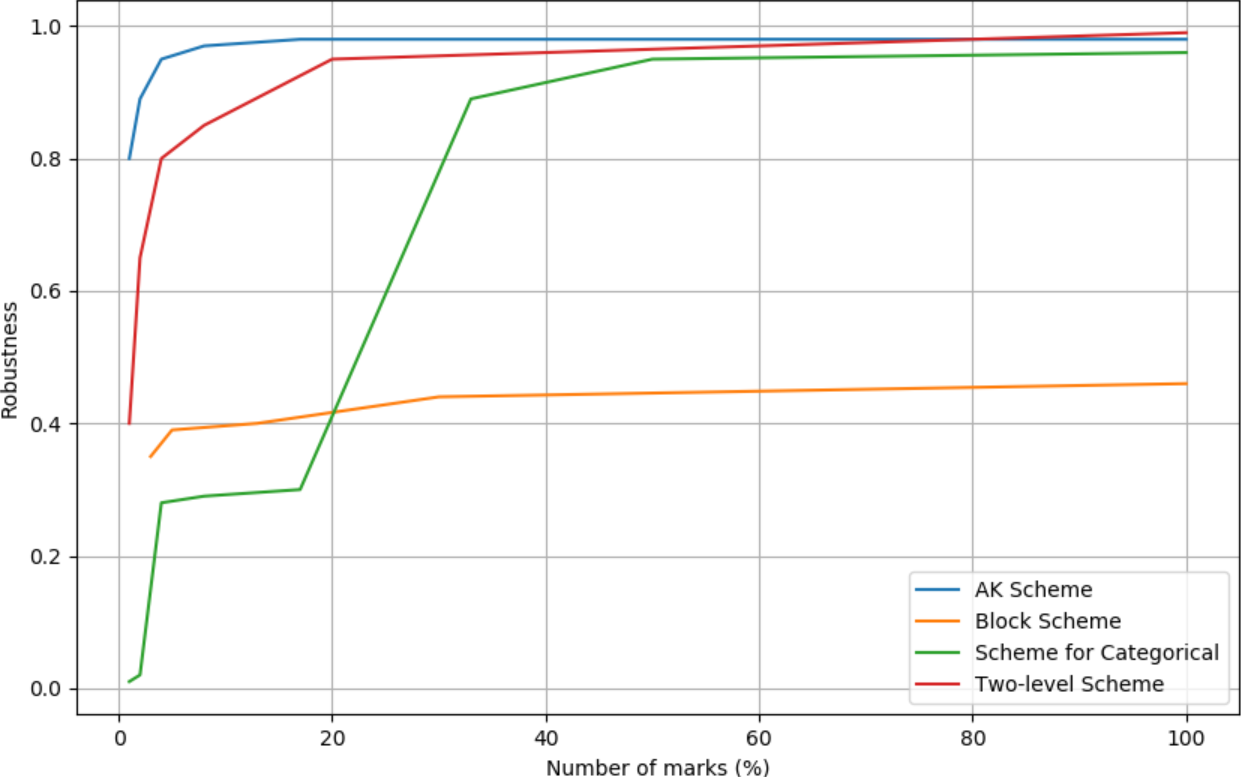
\includegraphics[width=\textwidth]{Figures/subset-screensh.PNG}
        \caption{Comparison of robustness against the subset attack}
        \label{fig:subset-attack}
    }\end{minipage}\hfill
    %bit-flipping
    \begin{minipage}{0.49\textwidth}
        \centering
        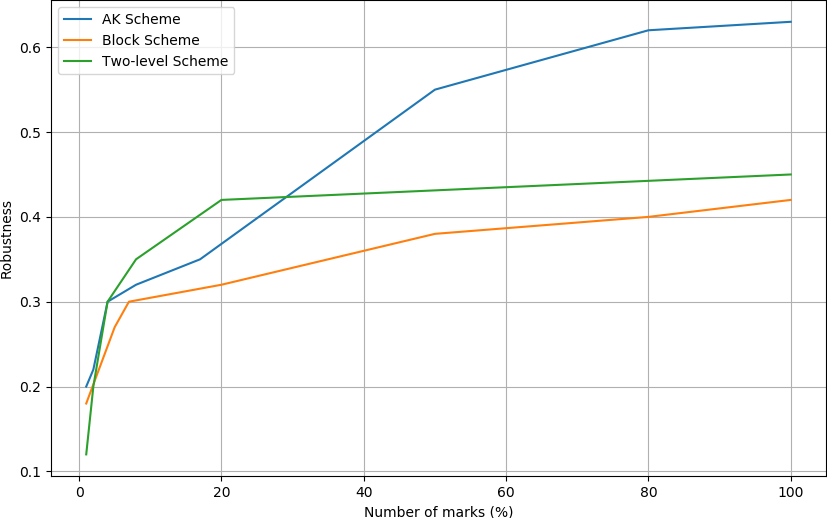
\includegraphics[width=\textwidth]{Figures/bit-flipping.PNG}
        \caption{Comparison of robustness against the bit-flipping attack}
        \label{fig:bit-flipping-attack}
    \end{minipage}
\end{figure}
Furthermore, we discussed the robustness against the attacks where the attacker modifies the dataset, e.g. subset attack and bit-flipping attack. A general conclusion is that more marks in the data mean better robustness. A somewhat smaller role plays the parameter $\xi$ that defines how many LSBs are available for fingerprinting such that is $\xi$ is bigger, the scheme is more robust. 
We compare the robustness of the discussed fingerprinting techniques against the subset attack in \Cref{fig:subset-attack} and the bit-flipping attack \Cref{fig:bit-flipping-attack}.
Robustness against the subset attack is measured as the largest percentage of tuples deleted where the scheme still detects the correct fingerprint with 100\% probability.
The AK Scheme shows the best robustness even for a smaller number of marks in the data. The Two-level Scheme and the scheme for categorical data are reaching a high robustness level for a larger number of marks in the data. The Block Scheme under-performs all the schemes.

Robustness of the bit-flipping attack is measured as the largest percentage of the LSBs that can be flipped while the scheme would still detect the correct fingerprint with probability 100\%.
AK Scheme again outperforms other schemes, except for the smaller number of marks where the Two-level Scheme is more robust. The Block Scheme is the least robust scheme against the bit-flipping attack. However, we can argue that all of the schemes are robust against the attack since they can all reach the level of robustness of $>0.4$.

We conclude that a good robustness level can be reached with a sufficient number of marks in the data. However, more marks in the data introduce more errors and they might significantly affect the utility of the data. In the next chapter, we will analyse how the utility is affected and if introducing the necessary number of marks to ensure the robustness is acceptable from the utility point of view.


\chapter{An evaluation on the utility of the fingerprinting schemes}\label{chapter:Utility}


\section{Quality effects on fingerprinted datasets}\label{sec:quality}
To get an insight into how the fingerprinting scheme affects the quality of the data that is disturbed by perturbations, we calculate the mean and variance of the values of an attribute. 
In this section, we first present the analysis and the empirical evaluation of changes in these two measures for each of the fingerprinting schemes described in \Cref{sec:Fingerprinting}. 
Exclusively, for the fingerprinting scheme for categorical data, we use a different quality measurement since the mean and variance do not apply to the categorical values. 
Instead, we count the number of changes in the data introduced by fingerprinting. 

\subsection{AK Scheme}
The procedure of embedding the fingerprint is determined by the owner's secret key $\mathcal{K}$, primary key attribute \textit{P} and controlled by parameters $\gamma$, \textit{v} and $\xi$.
In a dataset with $\eta$ tuples, on average $\eta/\gamma$ tuples are selected for marking. 
In a selected tuple a single bit of a single attribute will be selected for marking. 
Mark value is calculated as a result of applying XOR function on fingerprint bit and pseudorandomly selected mask bit.
The mark bit value will half of the times match the original value, on average, and therefore leave the selected bit unchanged.
Considering that the probability of selecting a value for marking is $1/(\gamma v)$, i.e. one over the number of selected tuples times number of attributes, and the probability that the mark bit differs from the original bit value is $1/2$, we obtain the probability that the value will be selected and changed

\begin{equation}
    P\{L_i=1\} = 1 - P\{L_i=0\} = \frac{1}{2\gamma v}
\end{equation}

where $L_i$ equals 1 if the value of a certain attribute of tuple \textit{i} is selected and changed (in contrast, it equals 0 if the new value doesn't differ from the original value).

In addition, we assume that the original values of an attribute in the dataset are $x_1,x_2,...,x_{\eta}$ and the values of the attribute after fingerprinting are $x_1+\Delta_1,x_2+\Delta_2,...,x_{\eta}+\Delta_{\eta}$. 
\{$\Delta_1,\Delta_2,...,\Delta_\eta$\} represent the error caused by fingerprinting.
They are independent and identically distributed random variables. 
We further assume the representation of $\Delta_i, 1 \leq i \leq \eta$, 

\begin{equation}
\Delta_i = L_i S_i 2^{U_i}
\end{equation}

where $S_i \in \{-1,1\}$ depending on whether the perturbed value is smaller or greater than the original, both with probability 0.5, and $U_i \in \{0,1,...,\xi-1\}$ is uniformly distributed variable representing position of the marked bit. 
\paragraph{Mean}
The mean value of the original attribute values is

\begin{equation}
\overline{x}=(1/\eta)\sum_{i=1}^{\eta}x_i
\end{equation}

and the mean of the attribute values after embedding the fingerprint is

\begin{equation}
\overline{x}'=\overline{x}+\overline{\Delta}
\end{equation} 

where

\begin{equation}
\overline{\Delta}=(1/\eta)\sum_{i=1}^{\eta} \Delta_i
\end{equation}

The expected error of a single attribute value is

\begin{equation}
E[\Delta_i]=\frac{1}{2} L_i 2^{U_i} - \frac{1}{2} L_i 2^{U_i} = 0, \forall i:1 \leq i \leq \eta
\end{equation}

thus the expected error in attribute mean value after embedding the fingerprint is 

\begin{equation}
E[\overline{\Delta}]=0
\end{equation}

\paragraph{Variance}
The variance of the original attribute values is given by 

\begin{equation}
V_x=\frac{1}{\eta}\sum_{i=1}^{\eta} (x_i - \overline{x})^2
\end{equation}

and the variance of the perturbed attribute values after the fingerprint insertion is 

\begin{equation}
V_{x+\Delta}=\frac{1}{\eta}\sum_{i=1}^{\eta}[(x_i+\Delta_i)-(\overline{x}+\overline{\Delta})]^2
\end{equation}

After applying some algebra, the error in variance is given by

\begin{equation}
V_{x+\Delta}-V_x = \frac{1}{\eta} \sum_{i=1}^{\eta}(\Delta_i-\overline{\Delta})^2 + 2\cdot\frac{1}{\eta}\sum_{i=1}^{\eta}(x_i-\overline{x})(\Delta_i-\overline{\Delta})
\end{equation}

The expected error in computing the variance is given by

\begin{equation}
E[V_\Delta]\approx\frac{2^{2\xi}}{6\gamma v \xi}
\end{equation}


\begin{table}[ht]
\centering
\caption{Change in variance introduced by fingerprinting with AK Scheme}
\label{table:AK-mean-var}
\resizebox{\textwidth}{!}{
\begin{tabular}{|lrr|rr|rr|rr|rr|} 
 \hline
 & & $\gamma$ & \multicolumn{2}{c|}{100} & \multicolumn{2}{c|}{50} & \multicolumn{2}{c|}{25} & \multicolumn{2}{c|}{12} \\ 
 & & $\xi$ & \multicolumn{1}{c}{4}&\multicolumn{1}{c|}{8}&\multicolumn{1}{c}{4}&\multicolumn{1}{c|}{8}&\multicolumn{1}{c}{4}&\multicolumn{1}{c|}{8}&\multicolumn{1}{c}{4}&\multicolumn{1}{c|}{8}\\
 \hline
 & \multicolumn{2}{c|}{Expected error in variance} & 0 & 1.4 & 0.01 & 2.7 & 0.02 & 5.5 & 0.04 & 11.4 \\
 \hline
 \textbf{Attribute} & \textbf{Mean} & \textbf{Variance} & & & & & & & & \\
 \hline
 Elevation & 2,959 & 78,391 & 0 &+1& 0 &+1&+1&+5&+1& +9 \\
 \hline
 Aspect & 156 & 12,525 &0 &+1&0 &+1&+1&+5& 0 & +8 \\
 \hline
 Slope & 14 & 56 & 0 &+1 &0 & +3&0 & +5&0  & +11 \\
 \hline
 HD-Hydrology & 269 & 45,177 &0 & +1& 0 &+1 &0 &+2 &+1  &+2  \\
 \hline
 VD-Hydrology & 46 & 3,398 & 0 & +1 & 0 & +2 &0 &+4 &0  &+9  \\
 \hline
 HD-Roadways & 2,350 & 2,431,276 & 0 & +10 & 0 & +10 & \textcolor{red}{-1} & +5 & +2  & +37  \\
 \hline
 Hillshade-9am & 212 & 717 & 0&+1 &0 &+2 &0 &+4 &  0 &+9  \\
 \hline
 Hillshade-noon & 223 & 391 & 0& +1&0 &+2 &0 &+4 &0  & +10 \\
 \hline
 Hillshade-3pm & 143 & 1,465 & 0& +1& 0&+2 &0 &+4 &0  &+8  \\
 \hline
 HD-Fire-Points & 1,980 & 1,753,493 & 0 & \textcolor{red}{-2} & 0 & +5 & 0 & +8 & +1 & +30  \\
 \hline
\end{tabular}
}
\end{table}

\paragraph{Experiments}
Experimental results are obtained by embedding a fingerprint into the Forest dataset. 
We choose the set of following values for parameter $\gamma$ = \{12,25,50,100\}, and $\xi$ = \{4,8\}. 
Table \ref{table:AK-mean-var} contains recorded changes in the variance introduced by fingerprinting for each of the attributes and parameter setting.
The results support the analysis previously made on errors in the mean and variance of the attribute values.
The error in the mean in all of the cases of this experiment was $<0.01$, so only the error in the variance is presented.
The largest changes are expectedly occurring when $\gamma$ is small and $\xi$ is big, i.e. when more tuples are selected and more bits of the value are available for marking. 
The errors in variance between cases with the same $\gamma$ value and different $\xi$ differ significantly, implying that imperceptibility of the fingerprint is highly sensitive to the number of LSBs available for marking.
Original values of the variances, in general, do not affect the relative error of perturbed values.  
In rare cases, the introduced errors result in a decrease of the variance, however, the change is in the same range as in cases where the variance increases. 


\subsection{Block Scheme}

Experimental results are obtained by embedding a fingerprint into the Forest dataset. 
We choose the set of following values for parameter $\beta$ = \{30,25,15,10\}, and $\xi$ = \{4,8\}. 
Table \Cref{table:block-mean} contains recorded changes in mean introduced by fingerprinting for each of the attributes and parameter setting, and \Cref{table:block-var} changes in variance.
\begin{table}[h]
\centering
\caption{Change in mean introduced by fingerprinting with the Block Scheme}
\label{table:block-mean}
\begin{tabular}{|l r|c c| c c| c c| c c|} 
 \hline
 & $\beta$ & \multicolumn{2}{c|}{30} & \multicolumn{2}{c|}{25} & \multicolumn{2}{c|}{15} & \multicolumn{2}{c|}{10} \\ 
 & $\xi$ &4&8&4&8&4&8&4&8\\
 \textbf{Attribute} & \textbf{Mean} & & & & & & & & \\
 \hline
 Elevation & 2959 &  &  &  &  &  &  &  & \\
 \hline
 Aspect & 156 &  &  &  &  &  &  &  & \\
 \hline
 Slope & 14 &  &  &  &  &  & +1 &  & \\
 \hline
 HD-Hydrology & 269 &  &  &  &  &  &  &  & \\
 \hline
 VD-Hydrology & 46 &  &  &  & +1 &  & +1 &  & +1\\
 \hline
 HD-Roadways & 2350 &  &  &  &  &  &  &  & \\
 \hline
 Hillshade-9am & 212 &  &  &  &  &  &  &  & \\
 \hline
 Hillshade-noon & 223 &  &  &  &  &  &  &  & \textcolor{red}{-2}\\
 \hline
 Hillshade-3pm & 143 &  &  &  & \textcolor{red}{-1} &  & \textcolor{red}{-1} &  & \textcolor{red}{-1}\\
 \hline
 HD-Fire-Points & 1980 &  &  &  &  &  &  &  & \\
 \hline
\end{tabular}
\end{table}

\begin{table}[ht]
\centering
\caption{Change in variance introduced by fingerprinting with the Block Scheme}
\label{table:block-var}
\begin{tabular}{|l r|r r|r r|r r|r r|} 
 \hline
 & $\beta$ & \multicolumn{2}{c|}{30} & \multicolumn{2}{c|}{25} & \multicolumn{2}{c|}{15} & \multicolumn{2}{c|}{10} \\ 
 & $\xi$ & \multicolumn{1}{c}{4}&\multicolumn{1}{c|}{8}&\multicolumn{1}{c}{4}&\multicolumn{1}{c|}{8}&\multicolumn{1}{c}{4}&\multicolumn{1}{c|}{8}&\multicolumn{1}{c}{4}&\multicolumn{1}{c|}{8}\\
 \textbf{Attribute} & \textbf{Variance} & & & & & & & & \\
 \hline
 Elevation & 78391 & 0 & +13 & +1 & +15 & +1 & +48 & +1 & +178 \\
 \hline
 Aspect & 12525 & 0 & +7 & 0 & +12 & 0 & +35 & 0 & +127 \\
 \hline
 Slope & 56 & 0 & +12 & 0 & +18 & 0 & +48 & 0 & 0 \\
 \hline
 HD-Hydrology & 45177 & 0 & +6 & +1 & +4 & +1 & +13 & +2 & 0 \\
 \hline
 VD-Hydrology & 3398 & 0 & +10 & 0 & +15 & 0 & +38 & 0 & +87 \\
 \hline
 HD-Roadways & 2431276 & 0 & +3 & 0 & +3 & 0 & +44 & \textcolor{red}{-2} & 0 \\
 \hline
 Hillshade-9am & 717 & 0 & +11 & 0 & +15 & 0 & +41 & 0 & +8 \\
 \hline
 Hillshade-noon & 391 & 0 & +11 & 0 & +16 & 0 & +45 & 0 & +200 \\
 \hline
 Hillshade-3pm & 1465 & 0 & 0 & 0 & +13 & 0 & +35 & 0 & +160 \\
 \hline
 HD-Fire-Points & 1753493 & 0 & 0 & 0 & \textcolor{red}{-4} & 0 & +54 & 0 & +68 \\
 \hline
\end{tabular}
\end{table}

The error is primarily controlled by parameter $\beta$. 
We have previously discussed the expected average number of changes which is described with \Cref{eq:block-changes}. 
$\beta$ in denominator suggests that for smaller $\beta$ there will be more errors in the data introduced by the fingerprint. 
We can see that a larger number of errors expectedly introduces larger errors in variance from the \Cref{table:block-var}.
The smallest error of variance appears for $\beta=30$ and increases for smaller $\beta$ values.

A large difference in the error of variance is noticeable between different values of $\xi$ which defines the number of LSBs available for fingerprinting.
We expect larger errors if more LSBs are available for fingerprinting - bits of more significance are being potentially changed, therefore creating bigger distortions (also assumed from \Cref{eq:block-changes}).
The experiment results in \Cref{table:two-level-mean-var} and \Cref{table:block-mean} confirm this claim. 
Setting $\xi=4$ will result in no or very small errors of variance and mean.
Note that $\xi=8$ may change a value in the dataset up to $\pm 2^7=\pm 128$. 
Considering that most of the values in Forest dataset are in the range of $2^7$, $\xi=8$ is a rather big value. 
For example, in the attribute \textit{Slope} where the mean value is 14 (see \Cref{table:block-mean}), this may cause quite a perceptible modification. 
For attributes with a range of larger values, e.g. \textit{Aspect} with mean 156 or \textit{HD-Roadways} with mean 2350, the error of $\leq \pm 128$ causes slightly less perceptible modifications in single values compared to \textit{Slope}, however the overall variance is certainly affected. 
We see in \Cref{table:block-mean} that error in the mean is introduced only for $\xi=8$ and for attributes with the small mean value.
We have set $\xi=8$ for experiments purely to show the clear distinction of the ways that different values of $\xi$ affect the quality of the data. 
In practice, $\xi$ is set according to the values in the dataset and generally to the smaller values. When $\xi$ is set appropriately, in these experiments $\xi=4$, different values of $\beta$ do not affect the errors in mean and variance too much.

\subsection{Two-level Fingerprinting Scheme}

The embedding process is controlled by $\gamma_1$, $\gamma_2$ and $\xi$.
Using \Cref{eq:total-gamma}, a dataset with $\eta$ tuples will have $ \frac{1}{\gamma}=\frac{1}{\gamma_1}+(1-\frac{1}{\gamma_1})*\frac{1}{\gamma_2}$ tuples selected for marking. Due to the pseudo-random nature of bit marking, the selected bit's original value will half of the times match the mark. 
Thus, the probability that the value will be selected and changed is
\begin{equation}
    P\{L_i=1\} = 1- P\{L_i=0\}=\frac{1}{2\gamma} = \frac{1}{2\gamma_1} +(1-\frac{1}{\gamma_1})*\frac{1}{2\gamma_2}
\end{equation}

where $L_i$ equals 1 if the value of a certain attribute of tuple \textit{i} is selected and changed (in contrast, it equals 0 if the new value doesn't differ from the original value).

The authors of the proposed scheme in their work \cite{guo2006fragile} present the quality effects by measuring mean and variance before and after embedding. 
They show the results from experiments run on a portion of Forest Cover data ($\eta=5,000$) and where fingerprinting is applied to a single attribute - \textit{Elevation}. 
Both mean and variance showed minor absolute alteration ($\approx0.01$) and lead to the conclusion that the scheme preserves the utility of the data. 

We show the empirical results on change in mean and variance in a scenario with entire Forest Cover Type data ($\eta=581,012$). 
For our experiments we consider all 10 numerical attributes for marking ($v=10$) and set parameters as follows: $\gamma_1=\gamma_2=\{10, 25, 50, 100\}$, $\eta=\{4, 8\}$ and $L=96$.

\begin{table}[ht]
\centering
\caption{Change in variance introduced by fingerprinting using the Two-level Fingerprinting Scheme}
\label{table:two-level-mean-var}
\resizebox{\textwidth}{!}{
\begin{tabular}{|lrr|rr|rr|rr|rr|} 
 \hline
 & & $\gamma_1=\gamma_2$ & \multicolumn{2}{c|}{100} & \multicolumn{2}{c|}{50} & \multicolumn{2}{c|}{25} & \multicolumn{2}{c|}{10} \\ 
 & & $\xi$ & \multicolumn{1}{c}{4}&\multicolumn{1}{c|}{8}&\multicolumn{1}{c}{4}&\multicolumn{1}{c|}{8}&\multicolumn{1}{c}{4}&\multicolumn{1}{c|}{8}&\multicolumn{1}{c}{4}&\multicolumn{1}{c|}{8}\\
 \textbf{Attribute} & \textbf{Mean} & \textbf{Variance} & & & & & & & & \\
 \hline
 Elevation & 2959 & 78391 &+1  & +3& +1& +4 & +1 & +4& +1 & +14\\
 \hline
 Aspect & 156 & 12525 &0 & +3 &0& +7& 0& +15&0 & +36\\
 \hline
 Slope & 14 & 56 &0 & +1 &0& +2&0& +4& 0 & +10\\
 \hline
 HD-Hydrology & 269 & 45177 &0&+3 &0& +5&+1& +7& +2 & +10\\
 \hline
 VD-Hydrology & 46 & 3398 & 0& +1&0& +1&0& +3& 0 & +6\\
 \hline
 HD-Roadways & 2350 & 2431276 & \textcolor{red}{-1}& +12&0& +27&0& +31& +1 & +61 \\
 \hline
 Hillshade-9am & 212 & 717 & 0 & 0 & 0& +1&0& +2&0 &+6\\
 \hline
 Hillshade-noon & 223 & 391 & 0& +4& 0& +9&0& +18& 0 & +43\\
 \hline
 Hillshade-3pm & 143 & 1465 &0 &+1 & 0& +3&0& +5&0 & +13\\
 \hline
 HD-Fire-Points & 1980 & 1753493 &+1 & 0 & +1& +12&0& +19& +1 & +34\\
 \hline
\end{tabular}}
\end{table}

The total mark ratio in the embedding process is around $1/\gamma_1 + 1/\gamma_2$. 
\Cref{table:two-level-mean-var} shows that the change in variance increases for larger number of marks, i.e. smaller $\gamma_1$ and $\gamma_2$. 
The change, however, depends on the number of LSBs available for marking $\xi$ as well. 
By choosing a smaller value, the change of variance can be almost completely avoided. The smaller $\xi$ value, however, decreases the robustness of the scheme which needs to be taken into account when choosing the value of this parameter. This is discussed in \Cref{sec:Robustness}.
The mean value of any attribute did not change more than $0.01$ in any of the experiments.
These changes are minuscule enough to hold the claim that the alteration for fingerprinting does not affect the usability of the data.


\subsection{Fingerprinting scheme for categorical data}
The fingerprinting scheme that deals with categorical data requires a different type of measure for data utility since mean and variance are not applicable in this case. One possible measure is the number of changes introduced by marking the data.

We fingerprint the categorical values of the Adult dataset using the fingerprinting scheme for categorical data. Furthermore, we fingerprint the numerical attributes using the AK Scheme. 
\Cref{table:categorical-ak-mean} shows the utility effects on the Adult dataset (which contains 30,162 tuples) introduced by the fingerprinting scheme for categorical data. 
The utility of numerical attributes is still measured by mean and variance, where the difference in the mean is negligible (it does not exceed 0.02 and is therefore excluded from the table). The change in variance introduced by errors for numerical attributes is also rather small, as it was the case with previously presented schemes. 
For each categorical attribute, we count how many changes in values are introduced by the fingerprint.
The Number of values that change in a single categorical attribute is approximately $30,162/(2\gamma v )$. 
For the presented set of parameters, the introduced total number of changes is $<4\%$ of the total number of tuples in the dataset. 
Due to the random nature of fingerprint insertion process, the distributions of attributes are not significantly affected.


\begin{table}[ht]
\centering
\caption{Change in variance and value-flips introduced by fingerprinting with the fingerprinting scheme for categorical data and the AK Scheme, on the Adult dataset}
\label{table:categorical-ak-mean}
\begin{tabular}{|l r|r r|r r|r r|r r|} 
 \hline
 & $\gamma$ & \multicolumn{2}{c|}{50} & \multicolumn{2}{c|}{25} & \multicolumn{2}{c|}{12} & \multicolumn{2}{c|}{6}
 \\ 
 & $\xi$ &2&4&2&4&2&4&2&4 \\

 \textbf{Attribute} & \textbf{Variance} & & & & & & & & \\
 \hline
 Age & 173 & 0 & 0 & 0 & 0 & 0 & 0 & 0 & +0.05 \\
 \hline
 Capital Gain & 54,853,968 & \textcolor{red}{-1} & \textcolor{red}{-3} & \textcolor{red}{-5} & \textcolor{red}{-11} & \textcolor{red}{-23} & \textcolor{red}{-56} & \textcolor{red}{-31} & \textcolor{red}{-67}\\
 \hline
 Capital Loss & 163,457 & 0 & \textcolor{red}{-1} & 0 & \textcolor{red}{-1} & \textcolor{red}{-1} & \textcolor{red}{-2} & \textcolor{red}{-2} & \textcolor{red}{-5} \\
 \hline
 Hours per Week & 144 & 0 & 0 & 0 & 0 & 0 & +0.2 & 0 & +0.3 \\
 \hline
  & & \multicolumn{8}{c|}{\textbf{Value Changes} }\\
\hline
 Workclass & & 26 & 19 & 45 & 45 & 81 & 90 & 165 & 165\\
 \hline
 Education && 26 & 18 & 49 &43 & 83 & 84 & 172 & 173\\
 \hline
 Marital Status && 24 & 24 & 46 & 44 & 101 & 87 & 207 & 189\\
 \hline
 Occupation && 23 & 20 & 44 & 47 & 75 & 73 & 148 & 135\\
 \hline
 Relationship && 22 & 22 & 29 & 41 & 81 & 89 & 175 & 189\\
 \hline
 Race && 19 & 20 & 47 & 51 & 87 & 91 & 160 & 174\\
 \hline
 Sex && 12 & 5 & 19 & 13 & 39 & 25 & 77 & 46\\
 \hline
 Native country && 19 & 21 & 45 & 30 & 94 & 78 & 173 & 164\\
 \hline
 \end{tabular}
 \end{table}


\section{Impact of fingerprinting on Machine Learning models}\label{sec:Learning}
In this section, we evaluate the utility of fingerprinted datasets by measuring the difference in the performance of classifiers for a predictive task, using the original and the fingerprinted dataset. 
We use \textit{accuracy} and \textit{F1} as performance measures. 
In Machine Learning, binary classification is the task of classifying the elements of a given set into two groups (also, categories or classes). 
Given a classification of a specific data set, there are four basic combinations of the actual data class and the assigned class: true positives (TP; actual positive and predicted positive), false positives (FP; actual negative and predicted positive), true negatives (TN; actual negative and predicted negative) and false negatives (FN; actual positive and predicted negative), where "positive" and "negative" represent two classes. 
These combinations can be arranged into a 2x2 contingency table as shown in \Cref{fig:confusion-matrix-binary}.

\begin{figure}
    \centering
    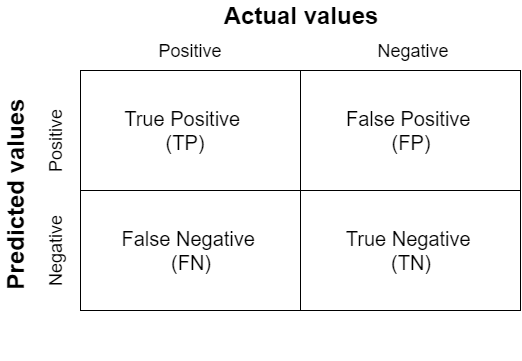
\includegraphics[width=0.6\textwidth]{Figures/confusion.png}
    \caption{Combinations of actual data classes and assigned classes in binary classification}
    \label{fig:confusion-matrix-binary}
\end{figure}

A calculation of the classification accuracy and F1 score is based on a number of occurrences of each combination in the classification. 
Accuracy is the ratio of a number of correct predictions to the total number of input samples.
Accuracy of a binary classification is defined as:
\begin{equation}\label{eq:accuracy-binary}
    accuracy = \frac{TP+TN}{P+N}
\end{equation}
where $P = TP+FP$ and $N = TN+FN$.
F1 score of binary classification is the harmonic average of the precision and the recall.
Precision, recall and F1 score for the binary classification are defined as follows:
\begin{equation}
    precision = \frac{TP}{TP+FP}
\end{equation}
\begin{equation}
    recall = \frac{TP}{TP+FN}
\end{equation}
\begin{equation}\label{eq:f1-binary}
    F1 = 2 \cdot \frac{precision \cdot recall}{precision + recall}
\end{equation}

The metrics are shown graphically in \Cref{fig:performance-metrics}.

\begin{figure}
    \centering
    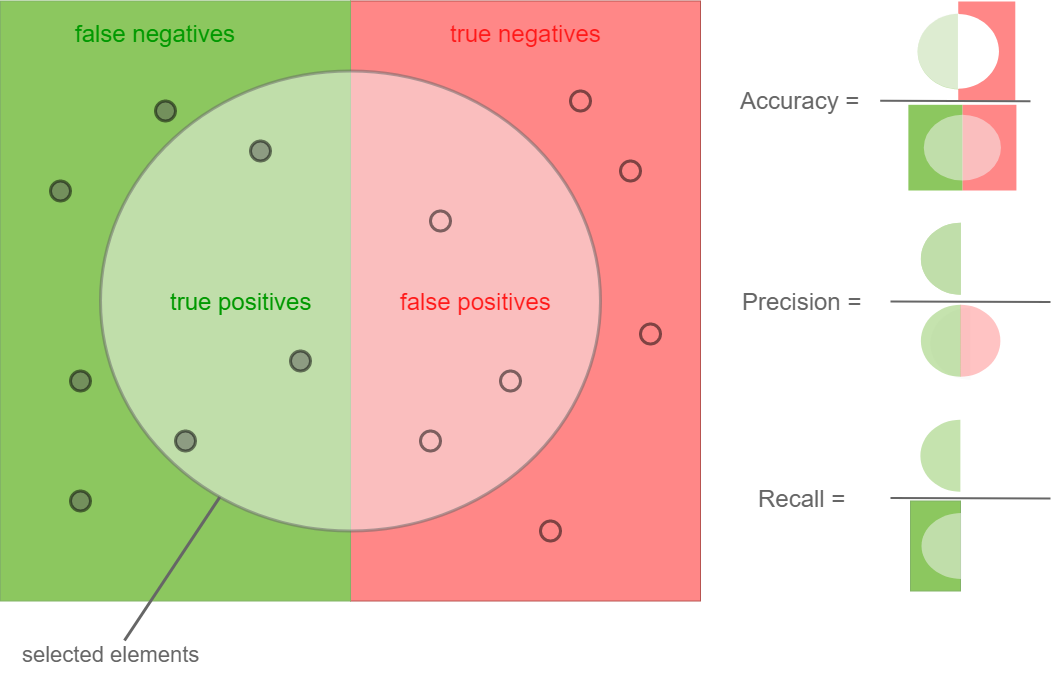
\includegraphics[width=0.8\textwidth]{Figures/metrics.png}
    \caption{Classification performance metrics}
    \label{fig:performance-metrics}
\end{figure}

Multiclass (or multinomial) classification is the task of classifying the elements of a given set into three or more groups (categories, classes). 
It can be denoted as a function $g(x)$ that on input $x$ returns one of the classes ${1,...,K}$.
Similarly to the binary classification, we can distinguish the combinations of actual data class and the predicted one. In this case, we have true positives, false positives and false negatives associated with each class $i$.
$\text{TP}_i$ denotes the instances from the class $i$ that are predicted to be in the class $i$, $\text{FP}_i$ are instances belonging to another class, falsely predicted to be in the class $i$, and $\text{FN}_i$ are the instances from the class $i$ falsely predicted to be in some other class. 

The accuracy of the multinomial classification is calculated as:
\begin{equation}\label{eq:accuracy-multiclass}
    accuracy = \frac{1}{\eta}\cdot \sum_{i=1}^{K}\text{TP}_i
\end{equation}
where $\eta$ is a total number of data instances. Note that \Cref{eq:accuracy-multiclass} is the general form that applies to the binary classification as well. 

For multiclass classification, precision and recall can be micro- or macro-averaged, therefore also can be F1 score.
The micro-averaged precision and recall are defined as follows:
\begin{equation}
    precision_{micro} = \frac{\sum_{i=1}^{K}\text{TP}_i}{\sum_{i=1}^{K}\text{TP}_i + \text{FP}_i}
\end{equation}
\begin{equation}
    recall_{micro} = \frac{\sum_{i=1}^{K}\text{TP}_i}{\sum_{i=1}^{K}\text{TP}_i + \text{FN}_i}
\end{equation}
Therefore, the micro F1 score is: 
\begin{equation}
    F1_{micro} = 2 \cdot \frac{precision_{micro} \cdot recall_{micro}}{precision_{micro} + recall_{micro}}
\end{equation}
If micro F1 is a large value, this indicates that a classifier performs well overall, however it is not sensitive to the performance of individual classes. 
The macro-averaged precision and recall are:
\begin{equation}
    precision_{macro} = \frac{1}{K}\sum_{i=1}^{K}\frac{\text{TP}_i}{\text{TP}_i + \text{FP}_i}
\end{equation}
\begin{equation}
    recall_{macro} = \frac{1}{K}\sum_{i=1}^{K}\frac{\text{TP}_i}{\text{TP}_i + \text{FN}_i}
\end{equation}
Hence, the macro F1 score is:
\begin{equation}\label{eq:f1-macro}
    F1_{macro} = 2 \cdot \frac{precision_{macro} \cdot recall_{macro}}{precision_{macro} + recall_{macro}}
\end{equation}
A large macro F1 suggests that the classifier performs well for each individual class. The macro-average is therefore more suitable for data with an imbalanced class distribution.
All of the above metrics reach their best value at 1 for the perfect classifier and worst at 0.

\paragraph{Experimental setup}
We used three datasets for the experiments - the Forest dataset, the Adult dataset and the Credit dataset. Therefore, three different classifications have been analysed. 
In the Forest dataset, the target attribute is \textit{covertype} with 7 values, thus we are solving the multiclass classification problem. 
The accuracy is calculated as in \Cref{eq:accuracy-multiclass}. Furthermore, we choose to use macro averages for calculating the F1 score (\Cref{eq:f1-macro}) to avoid the misleading nature of micro averages when the class distribution is imbalanced.

In the Adult dataset, we are predicting the binary attribute \textit{income}. In the German Credit dataset, we are as well predicting the binary target attribute that classifies the data instance as good or bad credit risk. The binary classification is being performed and analysed for these two datasets and accordingly, the classification accuracy and F1 are calculated as \Cref{eq:accuracy-binary} and \Cref{eq:f1-binary}.

For all of our experiments, we use 10-fold cross-validation to evaluate Machine Learning models.
$k$-fold cross-validation is a resampling procedure used in Machine Learning to estimate the skill of a Machine Learning model on unseen data.
It generally results in a less biased or less optimistic estimate of the model skill than other methods, such as a simple train/test split. 
The procedure starts by shuffling the dataset randomly and splitting it into $k$ groups. In our experiments $k=10$. 
Each unique group is taken as a hold out (test dataset) while the remaining $k-1$ groups are taken as a training dataset.
It fits a model on the training set and evaluates it on the test set, retaining the evaluation score for that group.
At the end, we summarise the skill of the model using the sample of model evaluation scores.
In the experiments, we record the average of these scores. 

Generally, the goal was not to build models with best predictions but to compare the effectiveness of the fingerprinted data compared to the original.
Therefore, there is no advanced parameter optimisation included nor we dive into more complicated feature selection for building models, as it would shift the focus from the main goal. 
Still, we wanted to achieve the model performance levels rather close to the benchmark solutions available from numerous online sources\footnote{\url{https://www.kaggle.com/wenruliu/adult-income-dataset/kernels}}\footnote{\url{https://www.kaggle.com/c/forest-cover-type-prediction/kernels}} (the chosen datasets and the correlated classification problems are well known in the Machine Learning community).
Therefore, it was important to find good hyperparameters for each of the classification tasks and each classifier.
One possible solution besides the pure manual tuning is a random search over hyperparameters.
We set up a grid of hyperparameter values and select a limited number of random combinations to train the model and score on validations data.
This way we choose the combination of parameters giving the best score for our model.

We use Randomized Search with 10 iterations from the Python scikit-learn package\footnote{\url{https://scikit-learn.org/stable/}} for tuning most important hyperparameters. 
Evaluation within the random search is done using 10-fold cross-validation and F1 score (macro F1 in case of a multiclass classification). 

Finally, for our experiments, we use the following classifiers, all implemented in the Python scikit-learn package:
\begin{itemize}
    \item Decision Tree
    \item k-NN (k Nearest Neighbours)
    \item Logistic regression
    \item Random Forest
    \item Gradient Boosting
\end{itemize}

The experimental process in the following sections has the following steps:
\begin{enumerate}
    \item Use random search to tune the hyperparameters of the Decision Tree, k-NN, Logistic Regression, Random Forest and Gradient Boosting classifiers. In some of the experiments, we use only the subset of the classifiers above. 
    \item Train the model with the original dataset and score the classification accuracy and F1
    \item For each fingerprinting parameter combination $(\gamma, \xi)$ train the model with the fingerprinted dataset and score the classification accuracy and F1. Set the hyperparameters according to step 1.  
    \item Record the differences in the performance measures
    \item Steps 3 and 4 are repeated 10 times to get the average values. In every experiment, we fingerprint the data with a random choice of buyer's id and secret key.
    
\end{enumerate}


% Forest dataset
\subsection{Forest Cover Type}
The first set of experiments is made using the biggest of the three datasets - Forest Cover Type. 
We use the AK Scheme for fingerprinting the numerical attributes of the dataset.
The target attribute is \textit{covertype} and all the others are used as an input for a prediction. 
We use the following classifiers and set the following hyperparameters:
    \begin{itemize}
        \item Decision Tree: $max\_depth=5$, $criterion=entropy$
        \item Logistic Regression: $C=100$
        \item Random Forest: $n\_estimators=100$
    \end{itemize}
    The other hyperparameters are set to default values from the scikit-learn implementations of the classifiers.

The average differences are shown in \Cref{tab:dt_forest_diff,tab:lr_forest_diff,tab:rf_forest_diff} for Decision Tree, Logistic Regression and Random Forest, respectively.

\begin{table}[ht]
    \centering
    \caption{Effects on F1 score and classification accuracy of a Decision Tree model trained with the Forest Cover Type dataset}
    \label{tab:dt_forest_diff}
    \resizebox{\textwidth}{!}{
    \begin{tabular}{|l|rr|rr|rr||rr|}
    \hline
        &  \multicolumn{2}{c|}{$\xi=2$} &  \multicolumn{2}{c|}{$\xi=4$} &  \multicolumn{2}{c||}{$\xi=6$} & 
        \multicolumn{2}{c|}{average} \\
        & F1 & acc. & F1 & acc.  & F1 & acc. & F1 & acc. \\
        \hline
         $\gamma=100$ & 0\% & 0\% & 0\% & \textcolor{red}{-0.01\%} & 0\% & \textcolor{red}{-0.01\%} & 0\% & \textcolor{red}{-0.01\%}\\
         \hline
         $\gamma=50$ & 0\% & \textcolor{red}{-0.02\%} & 0\% & 0\% & 0\% & +0.01\% & 0\% & 0\%\\
         \hline
         $\gamma=25$ & 0\% & \textcolor{red}{-0.02\%} & +0.02\% & +0.01\% & \textcolor{red}{-0.03\%} & \textcolor{red}{-0.01\%} & 0\% & \textcolor{red}{-0.01\%}\\
         \hline
         $\gamma=12$ & \textcolor{red}{-0.01\%} & \textcolor{red}{-0.02\%} & \textcolor{red}{-0.01\%} & 0\% & \textcolor{red}{-0.01\%} & \textcolor{red}{-0.10\%} & \textcolor{red}{-0.01\%} & \textcolor{red}{-0.04\%}\\
         \hline
         $\gamma=6$ & \textcolor{red}{-0.01\%} & 0\% & \textcolor{red}{-0.04\%} & \textcolor{red}{-0.01\%} & \textcolor{red}{-0.19\%} & \textcolor{red}{-0.11\%} & \textcolor{red}{-0.08\%} & \textcolor{red}{-0.04\%}\\
         \hline
         \hline
         average & 0\% & \textcolor{red}{-0.1\%} & \textcolor{red}{-0.01\%} & 0\% & \textcolor{red}{-0.05\%} & \textcolor{red}{-0.04\%} & \textbf{\textcolor{red}{-0.07\%}} & \textbf{\textcolor{red}{-0.02\%}}\\
         \hline
    \end{tabular}}
\end{table}


\begin{table}[ht]
    \centering
    \caption{Effects on F1 score and classification accuracy of a Logistic Regression model trained with the Forest Cover Type dataset}
    \label{tab:lr_forest_diff}
    \resizebox{\textwidth}{!}{
    \begin{tabular}{|l|rr|rr|rr||rr|}
    \hline
        &  \multicolumn{2}{c|}{$\xi=2$} &  \multicolumn{2}{c|}{$\xi=4$} &  \multicolumn{2}{c||}{$\xi=6$} & 
        \multicolumn{2}{c|}{average} \\
        & F1 & acc. & F1 & acc. & F1 & acc. & F1 & acc. \\
        \hline
         $\gamma=100$  & 0\% & 0\% & +0.01\% & 0\% & \textcolor{red}{-0.01\%} & +0.01\% & 0\% & 0\%\\
         \hline
         $\gamma=50$ & \textcolor{red}{-0.02\%} & 0\% & +0.01\% & 0\% & \textcolor{red}{-0.01\%} & +0.01\% & \textcolor{red}{-0.01\%} & 0\% \\
         \hline
         $\gamma=25$  & 0\% & 0\% & \textcolor{red}{-0.01\%} & \textcolor{red}{-0.01\%} & \textcolor{red}{-0.05\%} & +0.02\% & \textcolor{red}{-0.02\%} & 0\%\\
         \hline
         $\gamma=12$  & 0\% & 0\% & \textcolor{red}{-0.02\%} & 0\% & \textcolor{red}{-0.11\%} & +0.02\% & \textcolor{red}{-0.04\%} & 0\%\\
         \hline
         $\gamma=6$  & 0\% & 0\% & \textcolor{red}{-0.03\%} & 0\% & \textcolor{red}{-0.14\%} & +0.03\% & \textcolor{red}{-0.06\%} & +0.01\% \\
         \hline
         \hline
         average & 0\% & 0\% & \textcolor{red}{-0.01\%} & 0\% & \textcolor{red}{-0.07\%} & +0.02\% & \textbf{\textcolor{red}{-0.03\%}} & \textbf{+0.01\%}\\
         \hline
    \end{tabular}}
\end{table}


\begin{table}[ht]
    \centering
    \caption{Effects on F1 score and classification accuracy of a Random Forest model trained with the Forest Cover Type dataset}
    \label{tab:rf_forest_diff}
    \resizebox{\textwidth}{!}{
    \begin{tabular}{|l|rr|rr|rr||rr|}
    \hline
        &  \multicolumn{2}{c|}{$\xi=2$} &  \multicolumn{2}{c|}{$\xi=4$} &  \multicolumn{2}{c||}{$\xi=6$} & \multicolumn{2}{c|}{average} \\
        & F1 & acc. & F1 & acc. & F1 & acc. & F1 & acc. \\
        \hline
         $\gamma=100$ & +0.01\% & \textcolor{red}{-0.03\%} & +0.01\% & \textcolor{red}{-0.05\%} & \textcolor{red}{-0.06\%} & \textcolor{red}{-0.08\%} & \textcolor{red}{-0.01\%} & \textcolor{red}{-0.05\%} \\

         \hline
         $\gamma=50$  & 0\% & 0\% & +0.01\% & +0.02\% & \textcolor{red}{-0.02\%} & \textcolor{red}{-0.03\%} & 0\% & 0\% \\ 
    
        \hline
         $\gamma=25$  & 0\% & \textcolor{red}{-0.01\%} & \textcolor{red}{-0.07\%} & \textcolor{red}{-0.03\%} & \textcolor{red}{-0.05\%} & \textcolor{red}{-0.03\%} & \textcolor{red}{-0.04\%} & \textcolor{red}{-0.02\%} \\ 
         
        \hline
         $\gamma=12$  & \textcolor{red}{-0.02\%} & 0\% & \textcolor{red}{-0.01\%} & 0\% & \textcolor{red}{-0.03\%} & \textcolor{red}{-0.05\%} & \textcolor{red}{-0.02\%} & \textcolor{red}{-0.02\%}\\ 

        \hline
         $\gamma=6$  & \textcolor{red}{-0.04\%} & \textcolor{red}{-0.08\%} & \textcolor{red}{-0.01\%} & \textcolor{red}{-0.03\%} & 0\% & \textcolor{red}{-0.01\%} & \textcolor{red}{-0.02\%} & \textcolor{red}{-0.04\%}\\ 
      
        \hline
        \hline
        average & \textcolor{red}{-0.01\%} & \textcolor{red}{-0.03\%} & \textcolor{red}{-0.01\%} & \textcolor{red}{-0.02\%} & \textcolor{red}{-0.03\%} & \textcolor{red}{-0.04\%} & \textbf{\textcolor{red}{-0.02\%}} & \textbf{\textcolor{red}{-0.03\%}} \\
        \hline
    \end{tabular}}
\end{table}

The changes in performance are generally very small (in most of the cases the difference is in the 4th decimal place of the absolute values), therefore we represent the changes as percentages in range (0-100\%). 
All of the results roughly follow the rule that the performance measures decrease when $\gamma$ decreases, i.e. more marks introduced in data. We can observe this behaviour in the last columns of every table where we calculate the average F1 score and accuracy for a fixed $\gamma$ 
Furthermore, a general rule holds that the performance slightly drops for larger $\xi$ values, i.e. more bits available for fingerprinting. This is due to larger distortions of particular values in the data.
This is shown in the last row of every table where we average out the F1 score and accuracy for a fixed $\xi$.
Every classifier from the experiments behaves very similarly in the means of performance decrease. Overall average F1 score and accuracy for every classifier is calculated from the experiment results and presented the bottom rightmost cell of each table. 

On the Forest Cover Type data, we can conclude that the differences observed when using the Decision Tree classifier (see \Cref{tab:dt_forest_diff}) are rather minute, and would not constitute a noticeable degradation of effectiveness. 
The trend is the same also for other classifiers, as can be seen in \Cref{tab:lr_forest_diff} for Logistic Regression, and \Cref{tab:rf_forest_diff} for Random Forest.
In a few cases, the classification results obtained even improved, for example, the accuracy of Logistic Regression trained by data fingerprinted using $\xi=6$, though by the same rather marginal order of magnitude as the observed decline. 



% Adult data
\subsection{Adult (Census Data)}
We make the set of experiments using the Adult dataset. The dataset is mostly composed of categorical values, thus we use the fingerprinting scheme for categorical data from \Cref{subsec:fingerprinting-scheme-categorical}.
The target of the classification task is \textit{income}.
All other attributes (including numerical, although we do not fingerprint them) are used for as an input for a classifier.
We use Decision Tree, k-NN, Logistic Regression and Gradient Boosting. The hyperparameters are set as follows:
    \begin{itemize}
        \item k-NN: $n\_neighbors=19$
        \item Logistic Regression: $solver=liblinear$, $C=20$
        \item Random Forest: $n\_estimators=200$, $max\_depth=15$, $criterion=gini$
        \item Gradient Boosting: $n\_estimators:=40$, $max\_depth=8$, $loss=deviance$, $criterion=mse$
    \end{itemize}

The differences in F1 and accuracy scores (on a scale $[0,100]\%$) between original and fingerprinted Adult dataset for Decision Tree, k-NN, Logistic Regression, Random Forest and Gradient Boosting are shown in \Cref{tab:knn_adult_diff,tab:lr_adult_diff,tab:rf_adult_diff,tab:gb_adult_diff}.

\begin{table}[ht]
    \centering
    \caption{Effects on F1 score and classification accuracy of a k-NN model trained with the Adult dataset}
    \label{tab:knn_adult_diff}
    \resizebox{\textwidth}{!}{
    \begin{tabular}{|c|rr|rr|rr|rr||rr|}
    \hline
        & \multicolumn{2}{c|}{$\xi=1$} &  \multicolumn{2}{c|}{$\xi=2$} &  \multicolumn{2}{c|}{$\xi=4$} &  \multicolumn{2}{c||}{$\xi=6$} &  \multicolumn{2}{c|}{average} \\
        & F1 & acc. & F1 & acc. & F1 & acc. & F1 & acc. & F1 & acc.\\
        \hline
         $\gamma=50$ & +0.05\% & +0.03\% & \textcolor{red}{-0.10\%} & \textcolor{red}{-0.05\%} & \textcolor{red}{-0.06\%} & \textcolor{red}{-0.02\%} & \textcolor{red}{-0.02\%} & +0.01\% & \textcolor{red}{-0.03\%} & \textcolor{red}{-0.01\%}\\
         \hline
         $\gamma=25$ & \textcolor{red}{-0.10\%} & \textcolor{red}{-0.05\%} & +0.05\% & +0.02\% & +0.07\% & +0.03\% & \textcolor{red}{-0.02\%} & +0.03\% & 0\% & \textcolor{red}{-0.01\%} \\
         \hline
         $\gamma=12$ & \textcolor{red}{-0.32\%} & \textcolor{red}{-0.19\%} & \textcolor{red}{-0.10\%} & \textcolor{red}{-0.06\%} & +0.02\% & +0.03\% & \textcolor{red}{-0.20\%} & \textcolor{red}{-0.04\%} & \textcolor{red}{-0.15\%} & \textcolor{red}{-0.07\%}\\
         \hline
         $\gamma=6$ & \textcolor{red}{-0.70\%} & \textcolor{red}{-0.42\%} & \textcolor{red}{-0.50\%} & \textcolor{red}{-0.22\%} & \textcolor{red}{-0.36\%} & \textcolor{red}{-0.15\%} & \textcolor{red}{-0.60\%} & \textcolor{red}{-0.21\%} & \textcolor{red}{-0.54\%} & \textcolor{red}{-0.25\%}\\
         \hline
         $\gamma=3$ & \textcolor{red}{-1.79\%} & \textcolor{red}{-1.02\%} & \textcolor{red}{-0.70\%} & \textcolor{red}{-0.36\%} & \textcolor{red}{-0.61\%} & \textcolor{red}{-0.22\%} & \textcolor{red}{-0.81\%} & \textcolor{red}{-0.32\%} & \textcolor{red}{-0.98\%} & \textcolor{red}{-0.48\%}\\
         \hline
         \hline
         average & \textcolor{red}{-0.57\%} & \textcolor{red}{-0.33\%} & \textcolor{red}{-0.27\%} & \textcolor{red}{-0.13\%} & \textcolor{red}{-0.19\%} & \textcolor{red}{-0.07\%} & \textcolor{red}{-0.33\%} & \textcolor{red}{-0.11\%} & \textbf{\textcolor{red}{-0.34\%}} & \textbf{\textcolor{red}{-0.16\%}}  \\
         \hline
    \end{tabular}}
\end{table}


\begin{table}[ht]
    \centering
    \caption{Effects on F1 score and classification accuracy of a Logistic Regression model trained with the Adult dataset}
    \label{tab:lr_adult_diff}
    \resizebox{\textwidth}{!}{
    \begin{tabular}{|c|rr|rr|rr|rr||rr|}
    \hline
        & \multicolumn{2}{c|}{$\xi=1$} &  \multicolumn{2}{c|}{$\xi=2$} &  \multicolumn{2}{c|}{$\xi=4$} &  \multicolumn{2}{c||}{$\xi=6$} & 
        \multicolumn{2}{c|}{average}\\
        & F1 & acc. & F1 & acc. & F1 & acc. & F1 & acc. & F1 & acc. \\
        \hline
         $\gamma=50$ & \textcolor{red}{-0.15\%} & \textcolor{red}{-0.07\%} & \textcolor{red}{-0.02\%} & \textcolor{red}{-0.01\%} & \textcolor{red}{-0.07\%} & \textcolor{red}{-0.03\%} & \textcolor{red}{-0.03\%} & \textcolor{red}{-0.02\%} & \textcolor{red}{-0.07\%} & \textcolor{red}{-0.03\%}\\
        \hline
         $\gamma=25$ & \textcolor{red}{-0.25\%} & \textcolor{red}{-0.14\%} & \textcolor{red}{-0.13\%} & \textcolor{red}{-0.06\%} & \textcolor{red}{-0.10\%} & \textcolor{red}{-0.06\%} & \textcolor{red}{-0.14\%} & \textcolor{red}{-0.06\%} & \textcolor{red}{-0.16\%} & \textcolor{red}{-0.08\%}\\
        \hline
         $\gamma=12$ & \textcolor{red}{-0.46\%} & \textcolor{red}{-0.22\%} & \textcolor{red}{-0.27\%} & \textcolor{red}{-0.12\%} & \textcolor{red}{-0.12\%} & \textcolor{red}{-0.08\%} & \textcolor{red}{-0.39\%} & \textcolor{red}{-0.15\%} & \textcolor{red}{-0.31\%} & \textcolor{red}{-0.14\%}\\
        \hline
         $\gamma=6$ & \textcolor{red}{-0.68\%} & \textcolor{red}{-0.38\%} & \textcolor{red}{-0.41\%} & \textcolor{red}{-0.22\%} & \textcolor{red}{-0.46\%} & \textcolor{red}{-0.19\%} & \textcolor{red}{-0.80\%} & \textcolor{red}{-0.33\%} & \textcolor{red}{-0.59\%} & \textcolor{red}{-0.28\%}\\
        \hline
         $\gamma=3$ & \textcolor{red}{-2.12\%} & \textcolor{red}{-1.01\%} & \textcolor{red}{-1.08\%} & \textcolor{red}{-0.52\%} & \textcolor{red}{-0.75\%} & \textcolor{red}{-0.32\%} & \textcolor{red}{-1.33\%} & \textcolor{red}{-0.62\%} & \textcolor{red}{-1.32\%} & \textcolor{red}{-0.62\%}\\
        \hline
        \hline
        average & \textcolor{red}{-0.73\%} & \textcolor{red}{-0.36\%} & \textcolor{red}{-0.38\%} & \textcolor{red}{-0.19\%} & \textcolor{red}{-0.25\%} & \textcolor{red}{-0.14\%} & \textcolor{red}{-0.54\%} & \textcolor{red}{-0.24\%} & \textbf{\textcolor{red}{-0.49\%}} & \textbf{\textcolor{red}{-0.23\%}} \\
        \hline
    \end{tabular}}
\end{table}


\begin{table}[ht]
    \centering
    \caption{Effects on F1 score and classification accuracy of a Random Forest model trained with the Adult dataset}
    \label{tab:rf_adult_diff}
    \resizebox{\textwidth}{!}{
    \begin{tabular}{|c|rr|rr|rr|rr||rr|}
    \hline
        & \multicolumn{2}{c|}{$\xi=1$} &  \multicolumn{2}{c|}{$\xi=2$} &  \multicolumn{2}{c|}{$\xi=4$} &  \multicolumn{2}{c||}{$\xi=6$} & \multicolumn{2}{c|}{average}\\
        & F1 & acc. & F1 & acc. & F1 & acc. & F1 & acc. & F1 & acc. \\
        \hline
         $\gamma=50$  & \textcolor{red}{-0.04\%} & +0.06\% & \textcolor{red}{-0.40\%} & \textcolor{red}{-0.10\%} & \textcolor{red}{-0.02\%} & +0.02\% & \textcolor{red}{-0.37\%} & \textcolor{red}{-0.09\%} & \textcolor{red}{-0.21\%} & \textcolor{red}{-0.03\%}\\
        \hline
         $\gamma=25$ & \textcolor{red}{-0.28\%} & \textcolor{red}{-0.13\%} & \textcolor{red}{-0.20\%} & \textcolor{red}{-0.03\%} & \textcolor{red}{-0.29\%} & \textcolor{red}{-0.08\%} & \textcolor{red}{-0.56\%} & \textcolor{red}{-0.15\%} & 
         \textcolor{red}{-0.33\%} & \textcolor{red}{-0.10\%} \\
        \hline
         $\gamma=12$ & \textcolor{red}{-0.59\%} & \textcolor{red}{-0.23\%} & \textcolor{red}{-0.63\%} & \textcolor{red}{-0.23\%} & \textcolor{red}{-0.13\%} & +0.02\% & \textcolor{red}{-0.34\%} & \textcolor{red}{-0.09\%} & \textcolor{red}{-0.42\%} & \textcolor{red}{-0.13\%}\\
        \hline
         $\gamma=6$ & \textcolor{red}{-0.68\%} & \textcolor{red}{-0.31\%} & \textcolor{red}{-0.66\%} & \textcolor{red}{-0.20\%} & \textcolor{red}{-0.33\%} & \textcolor{red}{-0.08\%} & \textcolor{red}{-0.76\%} & \textcolor{red}{-0.24\%} & \textcolor{red}{-0.61\%} & \textcolor{red}{-0.27\%}\\
        \hline
         $\gamma=3$ & \textcolor{red}{-2.26\%} & \textcolor{red}{-1.02\%} & \textcolor{red}{-1.04\%} & \textcolor{red}{-0.37\%} & \textcolor{red}{-1.24\%} & \textcolor{red}{-0.40\%} & \textcolor{red}{-1.01\%} & \textcolor{red}{-0.35\%} & \textcolor{red}{-1.39\%} & \textcolor{red}{-0.54\%}\\
        \hline
        \hline
        average & \textcolor{red}{-0.77\%} & \textcolor{red}{-0.33\%} & \textcolor{red}{-0.59\%} & \textcolor{red}{-0.19\%} & \textcolor{red}{-0.40\%} & \textcolor{red}{-0.10\%} & \textcolor{red}{-0.61\%} & \textcolor{red}{-0.18\%} & \textbf{\textcolor{red}{-0.69\%}} & \textbf{\textcolor{red}{-0.20\%}} \\
        \hline
    \end{tabular}}
\end{table}



\begin{table}[ht]
    \centering
    \caption{Effects on F1 score and classification accuracy of a Gradient Boosting model trained with the Adult dataset}
    \label{tab:gb_adult_diff}
    \resizebox{\textwidth}{!}{
    \begin{tabular}{|c|rr|rr|rr|rr||rr|}
    \hline
        & \multicolumn{2}{c|}{$\xi=1$} &  \multicolumn{2}{c|}{$\xi=2$} &  \multicolumn{2}{c|}{$\xi=4$} &  \multicolumn{2}{c||}{$\xi=6$} & \multicolumn{2}{c|}{average} \\
        & F1 & acc. & F1 & acc. & F1 & acc. & F1 & acc. & F1 & acc.\\
        \hline
         $\gamma=50$ & \textcolor{red}{-0.12\%} & \textcolor{red}{-0.06\%} & \textcolor{red}{-0.32\%} & \textcolor{red}{-0.16\%} & +0.02\% & \textcolor{red}{-0.01\%} & \textcolor{red}{-0.17\%} & \textcolor{red}{-0.07\%} &
         \textcolor{red}{-0.15\%} & \textcolor{red}{-0.08\%}\\
         \hline 
         $\gamma=25$ & \textcolor{red}{-0.40\%} & \textcolor{red}{-0.19\%} & \textcolor{red}{-0.43\%} & \textcolor{red}{-0.20\%} & \textcolor{red}{-0.13\%} & \textcolor{red}{-0.08\%} & \textcolor{red}{-0.30\%} & \textcolor{red}{-0.10\%} &
         \textcolor{red}{-0.32\%} & \textcolor{red}{-0.14\%}\\
         \hline 
         $\gamma=12$ & \textcolor{red}{-0.71\%} & \textcolor{red}{-0.34\%} & \textcolor{red}{-0.51\%} & \textcolor{red}{-0.18\%} & \textcolor{red}{-0.42\%} & \textcolor{red}{-0.18\%} & \textcolor{red}{-0.29\%} & \textcolor{red}{-0.11\%} &
         \textcolor{red}{-0.48\%} & \textcolor{red}{-0.20\%}\\
         \hline 
         $\gamma=6$ & \textcolor{red}{-0.85\%} & \textcolor{red}{-0.45\%} & \textcolor{red}{-0.74\%} & \textcolor{red}{-0.35\%} & \textcolor{red}{-0.39\%} & \textcolor{red}{-0.20\%} & \textcolor{red}{-0.69\%} & \textcolor{red}{-0.30\%} &
         \textcolor{red}{-0.67\%} & \textcolor{red}{-0.33\%}\\
         \hline 
         $\gamma=3$ & \textcolor{red}{-2.60\%} & \textcolor{red}{-1.22\%} & \textcolor{red}{-1.18\%} & \textcolor{red}{-0.59\%} & \textcolor{red}{-0.76\%} & \textcolor{red}{-0.36\%} & \textcolor{red}{-0.59\%} & \textcolor{red}{-0.27\%} & 
         \textcolor{red}{-1.28\%} & \textcolor{red}{-0.61\%} \\
         \hline
         \hline
         average & \textcolor{red}{-0.94\%} & \textcolor{red}{-0.45\%} & \textcolor{red}{-0.64\%} & \textcolor{red}{-0.30\%} & \textcolor{red}{-0.34\%} & \textcolor{red}{-0.17\%} & \textcolor{red}{-0.41\%} & \textcolor{red}{-0.17\%} & \textbf{\textcolor{red}{-0.58\%}} & \textbf{\textcolor{red}{-0.27\%}}\\
         \hline
    \end{tabular}}
\end{table}

Overall, each classifier shows a decrease in performance when the fingerprint is applied. 
Except for a few cases where the performance slightly improves, both F1 and accuracy decrease up to approximately 2\%. 
The average difference for each classifier can be seen in the respective table in the rightmost cell of the last row in bold characters. 
The largest average difference for the entire classifier is the change in F1 score of Gradient Boosting, -0.58\% (\Cref{tab:gb_adult_diff}). Therefore, we can argue that changes in F1 and accuracy in this range are rather acceptable. This is, of course, dependable on the use case. However, we need to consider that fingerprinting necessarily changes the values in the dataset and the performance can not be exactly the same as when the original dataset is used. 
The occurrences of the positive differences (see, for example, \Cref{tab:lr_adult_diff}, $\gamma=50$, $\xi=1$) are random and minute, and therefore concluding that a fingerprint in the data improves the performance of the Machine Learning model is a rule for certain cases would be wrong.

In the last row and the last column of every table, we calculate the average difference for the fixed $\xi$ or $\gamma$, respectively, to see the effects of these parameters more easily.
It is hard to detect any pattern between average values of F1/accuracy and $\xi$ value for any of the classifiers. 
This behaviour can be expected because bigger $\xi$ do not imply "more change" in values for this fingerprinting scheme compared to the schemes for numerical values.
For instance, using $\xi=3$ in fingerprinting could change a value "9" to "13" (difference of 4), while using $\xi=1$ could only (and at most!) change it to "8" (difference of 1). 
This behaviour does not apply to categorical data since the change from any categorical value to another is unit.
Therefore, the effect of the parameter $\xi$ on the performance of a model trained using fingerprinted data in classification is random. 

On the other hand, we can see the trend of a decrease in performance for smaller values of $\gamma$ in the last column of the tables. Both average F1 and accuracy gradually decrease for smaller $\gamma$, i.e. more marks in the dataset. It is the case for a majority of the particular cases with one fixed value of $\xi$. For example, the entire experimental results with Logistic Regression, in \Cref{tab:lr_adult_diff}, have a perfect inversely proportional relation between a value of $\gamma$ and absolute difference in F1 score or accuracy.

On the Adult dataset we can conclude that, from the classification point of view, the utility of data is preserved after applying the proposed fingerprinting technique for categorical data. The performance drops are not significant and can be controlled by the parameter $\gamma$. 

% German Credit Data
\subsection{German Credit Data}
With the last set of experiments, we analyse the utility of the fingerprinted data that contains a mixture of numerical and non-numerical attributes.
We use the German Credit dataset and apply both AK Scheme to the numerical values and the naive fingerprinting technique for categorical data to non-numerical. 
We unify these two processes into one fingerprinting process since these techniques share the algorithmic steps, except for the modification for marking the categorical values. 
We use Decision Tree, k-NN, Logistic Regression and Random Forest for the classification and follow the usual procedure. We find with the random search that the best hyperparameters for the model trained with original data are as follows:
\begin{itemize}
    \item Decision Tree: $max\_depth=2$, $criterion=entropy$
    \item k-NN: $n\_neighbors=14$
    \item Logistic Regression: $solver=newton-cg$, $C=70$
    \item Random Forest: $n\_estimators=85$, $max\_depth=10$, $criterion=gini$
\end{itemize}

\Cref{tab:dt_german_diff,tab:knn_german_diff,tab:lr_german_diff,tab:rf_german_diff} show the resulting differences in F1 and accuracy scores (on a scale $[0,100]\%$) between original and fingerprinted German Credit data for Decision Tree, k-NN, Logistic Regression and Random Forest, respectively.

\begin{table}[ht]
    \centering
    \caption{Effects on F1 score and classification accuracy of a Decision Tree model trained with the German Credit dataset}
    \label{tab:dt_german_diff}
    \resizebox{\textwidth}{!}{
    \begin{tabular}{|c|rr|rr|rr|rr||rr|}
    \hline
        &  \multicolumn{2}{c|}{$\xi=1$} &  \multicolumn{2}{c|}{$\xi=2$} &  \multicolumn{2}{c|}{$\xi=4$} &  \multicolumn{2}{c||}{$\xi=6$} & \multicolumn{2}{c|}{average}\\
        & F1 & acc. & F1 & acc. & F1 & acc. & F1 & acc. & F1 & acc. \\
        \hline
         $\gamma=12$ & 0\% & 0\% & \textcolor{red}{-0.07\%} & \textcolor{red}{-0.10\%} & \textcolor{red}{-0.07\%} & \textcolor{red}{-0.10\%} & 0\% & 0\% & \textcolor{red}{-0.04\%} & \textcolor{red}{-0.05\%}\\
        \hline
         $\gamma=9$ & 0\% & 0\% & 0\% & 0\% & \textcolor{red}{-0.14\%} & \textcolor{red}{-0.20\%} & \textcolor{red}{-0.14\%} & \textcolor{red}{-0.20\%} & \textcolor{red}{-0.07\%} & \textcolor{red}{-0.10\%}\\
        \hline
         $\gamma=6$ & 0\% & 0\% & \textcolor{red}{-0.07\%} & \textcolor{red}{-0.10\%} & \textcolor{red}{-0.14\%} & \textcolor{red}{-0.20\%} & \textcolor{red}{-0.14\%} & \textcolor{red}{-0.20\%} & \textcolor{red}{-0.09\%} & \textcolor{red}{-0.13\%}\\
        \hline
         $\gamma=3$ & 0\% & 0\% & \textcolor{red}{-0.14\%} & \textcolor{red}{-0.20\%} & \textcolor{red}{-0.14\%} & \textcolor{red}{-0.20\%} & \textcolor{red}{-0.42\%} & \textcolor{red}{-0.60\%} & \textcolor{red}{-0.18\%} & \textcolor{red}{-0.25\%}\\
        \hline
        \hline
    average & 0\% & 0\% & \textcolor{red}{-0.07\%} & \textcolor{red}{-0.10\%} & \textcolor{red}{-0.12\%} & \textcolor{red}{-0.18\%} & \textcolor{red}{-0.18\%} & \textcolor{red}{-0.25\%} & \textbf{\textcolor{red}{-0.09\%}} & \textbf{\textcolor{red}{-0.13\%}} \\
    \hline
    \end{tabular}}
\end{table}


\begin{table}[ht]
    \centering
    
    \caption{Effects on F1 score and classification accuracy of a k-NN model trained with the German Credit dataset}
    \label{tab:knn_german_diff}
    \resizebox{\textwidth}{!}{
    \begin{tabular}{|c|rr|rr|rr|rr||rr|}
    \hline
        &  \multicolumn{2}{c|}{$\xi=1$} &  \multicolumn{2}{c|}{$\xi=2$} &  \multicolumn{2}{c|}{$\xi=4$} &  \multicolumn{2}{c||}{$\xi=6$} & \multicolumn{2}{c|}{average} \\
        & F1 & acc. & F1 & acc. & F1 & acc. & F1 & acc.  & F1 & acc. \\
        \hline
         $\gamma=12$ & 0.0\% & 0.0\% & \textcolor{red}{-0.14\%} & \textcolor{red}{-0.20\%} & \textcolor{red}{-0.07\%} & \textcolor{red}{-0.10\%} & 0.0\% & 0.0\% & \textcolor{red}{-0.05\%} & \textcolor{red}{-0.08\%}\\
        \hline
         $\gamma=9$ & 0.0\% & 0.0\% & \textcolor{red}{-0.05\%} & \textcolor{red}{-0.10\%} & \textcolor{red}{-0.14\%} & \textcolor{red}{-0.20\%} & \textcolor{red}{-0.22\%} & \textcolor{red}{-0.30\%} & \textcolor{red}{-0.10\%} & \textcolor{red}{-0.15\%}\\
        \hline
         $\gamma=6$ & 0.0\% & 0.0\% & \textcolor{red}{-0.27\%} & \textcolor{red}{-0.40\%} & \textcolor{red}{-0.14\%} & \textcolor{red}{-0.20\%} & \textcolor{red}{-0.22\%} & \textcolor{red}{-0.30\%} & \textcolor{red}{-0.16\%} & \textcolor{red}{-0.23\%} \\
        \hline
         $\gamma=3$ & 0.0\% & 0.0\% & \textcolor{red}{-0.09\%} & \textcolor{red}{-0.10\%} & \textcolor{red}{-0.39\%} & \textcolor{red}{-0.60\%} & \textcolor{red}{-0.45\%} & \textcolor{red}{-0.60\%} & \textcolor{red}{-0.23\%} & \textcolor{red}{-0.33\%}\\
        \hline
        \hline
        average & 0\% & 0\% & \textcolor{red}{-0.14\%} & \textcolor{red}{-0.20\%} & \textcolor{red}{-0.19\%} & \textcolor{red}{-0.28\%} & \textcolor{red}{-0.22\%} & \textcolor{red}{-0.30\%} & \textbf{\textcolor{red}{-0.14\%}} & \textbf{\textcolor{red}{-0.19\%}}\\
        \hline
    \end{tabular}}
\end{table}

\begin{table}[ht]
    \centering
    \caption{Effects on F1 score and classification accuracy of a Logistic Regression model trained with the German Credit dataset}
    \label{tab:lr_german_diff}
    \resizebox{\textwidth}{!}{
    \begin{tabular}{|c|rr|rr|rr|rr||rr|}
    \hline
        &  \multicolumn{2}{c|}{$\xi=1$} &  \multicolumn{2}{c|}{$\xi=2$} &  \multicolumn{2}{c|}{$\xi=4$} &  \multicolumn{2}{c||}{$\xi=6$} & \multicolumn{2}{c|}{average} \\
        & F1 & acc. & F1 & acc. & F1 & acc. & F1 & acc. & F1 & acc. \\
        \hline
         $\gamma=12$ & \textcolor{red}{-0.02\%} & 0.0\% & \textcolor{red}{-0.45\%} & \textcolor{red}{-0.61\%} & \textcolor{red}{-0.02\%} & +0.09\% & +0.17\% & +0.30\% & \textcolor{red}{-0.08\%} & \textcolor{red}{-0.06\%} \\ 
         \hline
         $\gamma=9$ & \textcolor{red}{-0.04\%} & 0.0\% & \textcolor{red}{-0.27\%} & \textcolor{red}{-0.30\%} & \textcolor{red}{-0.38\%} & \textcolor{red}{-0.60\%} & \textcolor{red}{-0.25\%} & \textcolor{red}{-0.50\%} & \textcolor{red}{-0.24\%} & \textcolor{red}{-0.35\%}\\
         \hline
         $\gamma=6$ & \textcolor{red}{-0.05\%} & \textcolor{red}{-0.10\%} & \textcolor{red}{-0.42\%} & \textcolor{red}{-0.71\%} & \textcolor{red}{-0.55\%} & \textcolor{red}{-0.80\%} & \textcolor{red}{-0.25\%} & \textcolor{red}{-0.40\%} & \textcolor{red}{-0.32\%} & \textcolor{red}{-0.50\%} \\
        \hline
        $\gamma=3$ & \textcolor{red}{-0.17\%} & \textcolor{red}{-0.30\%} & \textcolor{red}{-0.26\%} & \textcolor{red}{-0.41\%} & \textcolor{red}{-0.21\%} & \textcolor{red}{-0.50\%} & \textcolor{red}{-0.29\%} & \textcolor{red}{-0.41\%} & \textcolor{red}{-0.23\%} & \textcolor{red}{-0.41\%} \\
         \hline
         \hline
         average & \textcolor{red}{-0.07\%} & \textcolor{red}{-0.10\%} & \textcolor{red}{-0.35\%} & \textcolor{red}{-0.51\%} & \textcolor{red}{-0.29\%} & \textcolor{red}{-0.45\%} & \textcolor{red}{-0.16\%} & \textcolor{red}{-0.25\%} & \textbf{\textcolor{red}{-0.22\%}} & \textbf{\textcolor{red}{-0.33\%}}\\
         \hline
    \end{tabular}}
\end{table}


\begin{table}[ht]
    \centering
    \caption{Effects on F1 score and classification accuracy of a decision Tree model trained with the Random Forest dataset}
    \label{tab:rf_german_diff}
    \resizebox{\textwidth}{!}{
    \begin{tabular}{|c|rr|rr|rr|rr||rr|}
    \hline
        &  \multicolumn{2}{c|}{$\xi=1$} &  \multicolumn{2}{c|}{$\xi=2$} &  \multicolumn{2}{c|}{$\xi=4$} &  \multicolumn{2}{c||}{$\xi=6$} & \multicolumn{2}{c|}{average} \\
        & F1 & acc. & F1 & acc. & F1 & acc. & F1 & acc.& F1 & acc. \\
        \hline
         $\gamma=12$ & \textcolor{red}{-0.47\%} & \textcolor{red}{-0.70\%} & \textcolor{red}{-0.81\%} & \textcolor{red}{-1.20\%} & \textcolor{red}{-0.07\%} & \textcolor{red}{-0.31\%} & \textcolor{red}{-0.21\%} & \textcolor{red}{-0.50\%} & \textcolor{red}{-0.39\%} & \textcolor{red}{-0.68\%}\\
        \hline
         $\gamma=9$ & \textcolor{red}{-0.50\%} & \textcolor{red}{-0.80\%} & \textcolor{red}{-0.34\%} & \textcolor{red}{-0.70\%} & \textcolor{red}{-0.31\%} & \textcolor{red}{-0.50\%} & \textcolor{red}{-0.35\%} & \textcolor{red}{-0.61\%} & \textcolor{red}{-0.38\%} & \textcolor{red}{-0.62\%} \\
        \hline
         $\gamma=6$ & \textcolor{red}{-0.82\%} & \textcolor{red}{-1.30\%} & \textcolor{red}{-0.42\%} & \textcolor{red}{-0.90\%} & \textcolor{red}{-0.44\%} & \textcolor{red}{-0.70\%} & \textcolor{red}{-0.30\%} & \textcolor{red}{-0.41\%} & \textcolor{red}{-0.50\%} & \textcolor{red}{-0.83\%}\\
        \hline
         $\gamma=3$ & \textcolor{red}{-0.79\%} & \textcolor{red}{-1.40\%} & \textcolor{red}{-0.78\%} & \textcolor{red}{-1.30\%} & \textcolor{red}{-1.23\%} & \textcolor{red}{-2.10\%} & \textcolor{red}{-0.85\%} & \textcolor{red}{-1.20\%} & \textcolor{red}{-0.91\%} & \textcolor{red}{-1.50\%} \\
        \hline
        \hline
        average & 
        \textcolor{red}{-0.65\%} & \textcolor{red}{-1.05\%} & \textcolor{red}{-0.59\%} & \textcolor{red}{-1.03\%} & \textcolor{red}{-0.51\%} & \textcolor{red}{-0.90\%} & \textcolor{red}{-0.43\%} & \textcolor{red}{-0.68\%} & \textbf{\textcolor{red}{-0.54\%}} & \textbf{\textcolor{red}{-0.91\%}} \\
        \hline
    \end{tabular}}
\end{table}

Similar to the Forest Cover Type dataset and Adult dataset, we can note that there are very small effects on the classification accuracy and F1 score using German Credit dataset. 

In experiments, the classification accuracy and F1 score generally slightly decrease for smaller $\gamma$, i.e. by introducing more error, which is expected. 
The effect of parameter $\xi$ is not obvious in all of the cases. We now have a mixture of numerical and non-numerical values. We have discussed in the previous sections that $\xi$ affects the performance when numerical data is used, while with non-numerical it is not the case. 
For example, results from Decision Tree in \Cref{tab:dt_german_diff} show the decrease in F1 and accuracy for larger $\xi$, while the results from Logistic Regression in \Cref{tab:lr_german_diff} do not show such relation.

Generally, bigger errors introduced by fingerprinting using the naive technique for categorical data did not significantly affect the performance of any of the classifiers. 

\paragraph{}
We further run experiments to analyse the second proposed technique for fingerprinting the categorical type of data. 
German Credit Data is fingerprinted using the approach of finding a fixed number of neighbours, with $k=10$. 
We use the same set values for parameters $\xi$ and $\gamma$ as in the previous experiments. 
We trained the Logistic Regression and the Random Forest models. The differences of the performance measures, classification accuracy and F1 score, are shown in \Cref{tab:lr_german_diff_novel,tab:rf_german_diff_novel}.


\begin{table}[ht]
    \centering
    \caption{Effects on F1 score and classification accuracy of a Logistic Regression model trained with the German Credit dataset fingerprinted with the neighbourhood-based technique}
    \label{tab:lr_german_diff_novel}
    \resizebox{\textwidth}{!}{
    \begin{tabular}{|c|rr|rr|rr|rr||rr|}
    \hline
        &  \multicolumn{2}{c|}{$\xi=1$} &  \multicolumn{2}{c|}{$\xi=2$} &  \multicolumn{2}{c|}{$\xi=4$} &  \multicolumn{2}{c||}{$\xi=6$} & \multicolumn{2}{c|}{average} \\
        & F1 & acc. & F1 & acc. & F1 & acc. & F1 & acc. & F1 & acc. \\
        \hline
         $\gamma=12$ & \textcolor{red}{-0.19\%} & \textcolor{red}{-0.20\%} & +0.03\% & +0.09\% & 0\% & \textcolor{red}{-0.01\%} & \textcolor{red}{-0.19\%} & \textcolor{red}{-0.30\%} & \textcolor{red}{-0.09\%} & \textcolor{red}{-0.11\%}\\
\hline
 $\gamma=9$ & \textcolor{red}{-0.24\%} & \textcolor{red}{-0.30\%} & \textcolor{red}{-0.23\%} & \textcolor{red}{-0.30\%} & 0\% & 0\% & \textcolor{red}{-0.34\%} & \textcolor{red}{-0.50\%} & \textcolor{red}{-0.20\%} & \textcolor{red}{-0.28\%} \\
\hline
 $\gamma=6$ & \textcolor{red}{-0.47\%} & \textcolor{red}{-0.60\%} & \textcolor{red}{-0.16\%} & \textcolor{red}{-0.31\%} & \textcolor{red}{-0.28\%} & \textcolor{red}{-0.41\%} & \textcolor{red}{-0.93\%} & \textcolor{red}{-1.31\%} & \textcolor{red}{-0.46\%} & \textcolor{red}{-0.66\%} \\
\hline
 $\gamma=3$ & \textcolor{red}{-0.65\%} & \textcolor{red}{-0.90\%} & \textcolor{red}{-0.33\%} & \textcolor{red}{-0.60\%} & +0.13\% & +0.09\% & \textcolor{red}{-0.07\%} & \textcolor{red}{-0.20\%} & \textcolor{red}{-0.23\%} & \textcolor{red}{-0.40\%}\\
\hline
\hline
average & \textcolor{red}{-0.39\%} & \textcolor{red}{-0.50\%} & \textcolor{red}{-0.17\%} & \textcolor{red}{-0.28\%} & \textcolor{red}{-0.04\%} & \textcolor{red}{-0.08\%} & \textcolor{red}{-0.38\%} & \textcolor{red}{-0.58\%} & \textcolor{red}{\textbf{-0.25\%}} & \textcolor{red}{\textbf{-0.36\%}} \\
\hline
    \end{tabular}}
\end{table}


\begin{table}[ht]
    \centering
    \caption{Effects on F1 score and classification accuracy of a Random Forest model trained with the German Credit dataset fingerprinted with the neighbourhood-based technique}
    \label{tab:rf_german_diff_novel}
    \resizebox{\textwidth}{!}{
    \begin{tabular}{|c|rr|rr|rr|rr||rr|}
    \hline
        &  \multicolumn{2}{c|}{$\xi=1$} &  \multicolumn{2}{c|}{$\xi=2$} &  \multicolumn{2}{c|}{$\xi=4$} &  \multicolumn{2}{c||}{$\xi=6$} & \multicolumn{2}{c|}{average}  \\
        & F1 & acc. & F1 & acc. & F1 & acc. & F1 & acc.& F1 & acc. \\
        \hline
         $\gamma=12$ & \textcolor{red}{-0.27\%} & \textcolor{red}{-0.60\%} & \textcolor{red}{-0.16\%} & \textcolor{red}{-0.50\%} & \textcolor{red}{-0.57\%} & \textcolor{red}{-1.10\%} & \textcolor{red}{-0.43\%} & \textcolor{red}{-1.00\%} & \textcolor{red}{-0.36\%} & \textcolor{red}{-0.80\%}\\
         
    \hline
    $\gamma=9$ & \textcolor{red}{-0.33\%} & \textcolor{red}{-0.60\%} & \textcolor{red}{-0.36\%} & \textcolor{red}{-0.70\%} & \textcolor{red}{-0.45\%} & \textcolor{red}{-0.90\%} & \textcolor{red}{-0.48\%} & \textcolor{red}{-0.90\%} & \textcolor{red}{-0.41\%} & \textcolor{red}{-0.78\%}\\
\hline
$\gamma=6$ & \textcolor{red}{-0.56\%} & \textcolor{red}{-1.00\%} & \textcolor{red}{-0.22\%} & \textcolor{red}{-0.40\%} & \textcolor{red}{-0.73\%} & \textcolor{red}{-1.31\%} & \textcolor{red}{-0.41\%} & \textcolor{red}{-0.90\%} & \textcolor{red}{-0.48\%} & \textcolor{red}{-0.90\%}\\
\hline
$\gamma=3$ & \textcolor{red}{-0.65\%} & \textcolor{red}{-1.10\%} & \textcolor{red}{-0.95\%} & \textcolor{red}{-1.90\%} & \textcolor{red}{-0.40\%} & \textcolor{red}{-0.90\%} & +0.01 & \textcolor{red}{-0.20\%} & \textcolor{red}{-0.50\%} & \textcolor{red}{-1.03\%}\\
\hline
\hline
average & \textcolor{red}{-0.45\%} & \textcolor{red}{-0.82\%} & \textcolor{red}{-0.42\%} & \textcolor{red}{-0.88\%} & \textcolor{red}{-0.54\%} & \textcolor{red}{-1.05\%} & \textcolor{red}{-0.33\%} & \textcolor{red}{-0.75\%} & \textcolor{red}{\textbf{-0.44\%}} & \textcolor{red}{\textbf{-0.88\%}} \\
\hline
    \end{tabular}}
\end{table}

The results are, generally, very similar to the results of the naive fingerprinting technique. 
The decrease in performance is in the range of approximately $-1\%$ for both classification accuracy and F1 score. 
The Logistic Regression gives overall slightly worse results in this case, while for the Random Forest the performance is slightly better compared to the naive technique. 
The performance follows the same trend of a decrease when more marks are embedded in the data. See, for example, the last column in \Cref{tab:rf_german_diff_novel} where we recorded the average F1 and accuracy decrease for different values of $\xi$. 
The difference is larger for smaller values of $\gamma$, i.e. more marks in the data. 




\section{Summary}
In this chapter, we deliver the analysis of the utility of the fingerprinted data. We analyse the utility from the two aspects. First, we measure the mean and variance of each attribute of the datasets before and after fingerprinting and compare them. Fingerprinting techniques for numerical data introduce almost no change in the mean and very little change in the variance. 
For the fingerprinting technique for non-numerical data where mean and variance are not applicable, we measure the quality by counting the number of changes. 

Secondly, we analyse the effect of the fingerprint on the classification performance.
We build Machine Learning models using the original dataset and record the performance scores. Then we record the performance scores of the models using the fingerprinted datasets, under the same set of hyperparameters.
The performance measures we use are the classification accuracy and F1 score.
Our experiments show that the decrease in performance is minute. The fingerprinting parameters, for example, the number of marks controlled by the parameter $\gamma$, influence the performance, however, the difference stays in the same range.
The example of the performance decrease depending on $\gamma$ is shown in \Cref{fig:classification-error} for Random Forest and three different datasets. 
The F1 score differences are reflected over the x-axis for clarity.
The trend of decrease in the performance error can be seen for fewer marks in data (bigger $\gamma$).
Furthermore, we can see that the range of the errors, both accuracy and F1, are within the range [0,1.5]\%, based on which we can argue that the error introduced by the fingerprint is negligible.
\begin{figure}
    \centering
    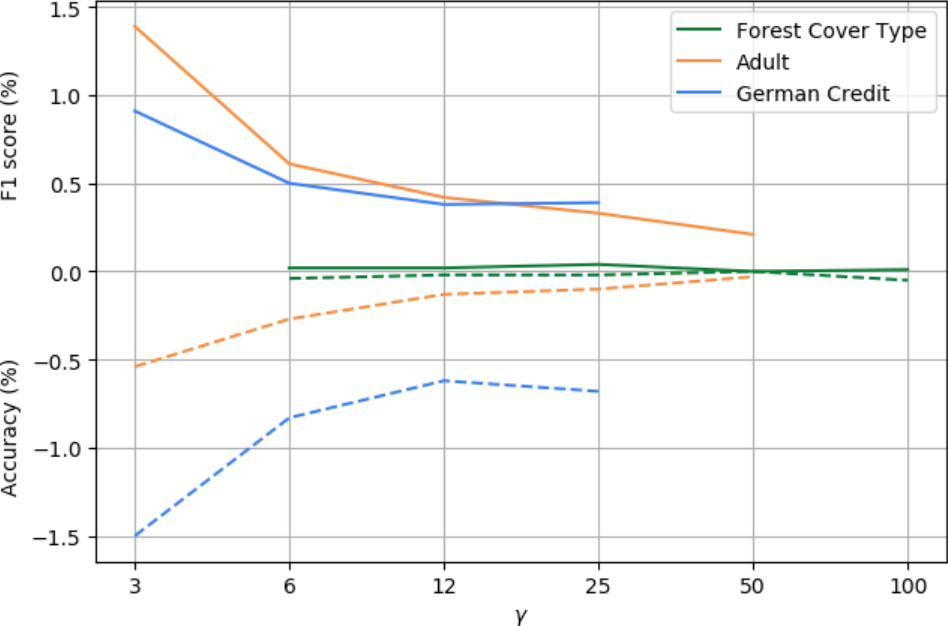
\includegraphics[width=0.8\textwidth]{Figures/classification-screenshot.PNG}
    \caption{Error in performance measures of the Random Forest classifier}
    \label{fig:classification-error}
\end{figure}

We obtain similar results with every other classifier, including Decision Tree, Logistic Regression, k-NN and Gradient Boosting. 
Our experiments with data fingerprinted with the second fingerprinting technique for categorical data based on finding the closest neighbourhood show very similar results to the naive approach. In future work, this technique will be more closely analysed, both from the robustness and the data utility point of view. In this case, the technique did not show distinctively better results than the naive approach. However, this might be case-specific and differ for the other choices of the parameter $k$ that defines the size of the neighbourhood. 


\chapter{Conclusion}\label{chapter:conclusion}
This thesis elaborates the concept of fingerprinting relational databases. 
We implement and analyse three fingerprinting techniques for relational data containing numerical values - AK Scheme, Block Scheme and Two-level Fingerprinting Scheme. 
The real-world datasets oftentimes contain non-numerical attributes. Therefore, we propose, implement and analyse two approaches for fingerprinting non-numerical data. The naive approach, inspired by techniques for fingerprinting numerical data, first converts the categorical attributes to numerical and then applies random marks on the chosen values. The second approach goes towards minimising contextual inconsistencies in the data after fingerprinting. 
Even though this technique is not blind, it might be a better solution for fingerprinting data with correlated categorical attributes than marking the values randomly.

We analyse the robustness of the techniques against the attacks. We analyse it theoretically and empirically, using the implemented techniques and a broad set of parameters. 
Attacks that modify the dataset without any background knowledge of where the marks are embedded and without the access to other copies of fingerprinted data (e.g. subset attack, superset attack, bit-flipping attack), are shown to be avoidable by careful parameter tuning. In most of the cases, the robustness is increased by increasing the number of marks in the data. 
If a smaller dataset is being fingerprinted, a fingerprinting scheme that creates shorter fingerprints is more robust. 

The AK Scheme appears to be the most robust technique among the analysed ones. This is beneficial for our choice that the proposed scheme for categorical data follows the same steps as the AK Scheme. 
The Two-level fingerprinting technique is very useful because of the verification of the ownership and the source of the leakage in two separate processes. 
The ownership verification level is much more robust to any kind of attack, which allows the owner to prove ownership even in cases when the exact fingerprint of the receiver cannot be extracted.
The Block Scheme is inspired by a useful fingerprinting technique for fingerprinting images, however, does not appear to be very robust in its adaptation to fingerprinting technique for relational datasets. 
The proposed technique for categorical data is less robust against the attacks than AK Scheme or Two-level Scheme, however still applicable.

We further analyse how the modifications in data affect its utility. 
The modifications in the mean and variance of the attributes are rather minute. More marks in data and more allowed bits for embedding the mark result in bigger variance errors.
The utility is further measured in the assumed scenario where the fingerprinted data is used for training a Machine Learning model that is making some prediction.
We use a variety of Machine Learning classifiers, including Decision Tree, Logistic Regression, k-NN, Random Forest and Gradient Boosting, and experiment with three different datasets. 
The resulting decrease of performance when compared to the model trained with original data is around 1\%, mostly less (assuming the accuracy and F1 score are measured in the range [0,100]\%). Therefore, the predictions are rather accurate when the fingerprinted data is used.

The parameters that would, for example, increase the robustness of the scheme, decrease the utility. 
We show in \Cref{tab:parameters} the effects of the main fingerprinting parameters on different types of attacks and the utility. 

\begin{table}[ht]
    \caption{Impact of parameters on robustness against attacks resp. on data utility}
    \label{tab:parameters}
    \centering
%    \renewcommand{\arraystretch}{1.5}
    \setlength{\tabcolsep}{6pt}  % default something like 2pt in this template
    \begin{tabular}{|l|c|c|c|c|c|}
        \hline
         $\bm{\uparrow}$ & $\omega$ & $\xi$ &  $\tau$ & $L$ & $N$  \\
         \hline
         Misdiagnosis false hit & $\bm{\uparrow}$ & & $\bm{\uparrow}$ & $\bm{\uparrow}$ & $\bm{\downarrow}$ \\
         \hline
         Subset Attack & $\bm{\uparrow}$ & & $\bm{\downarrow}$ & $\bm{\downarrow}$ & \\
         \hline
         Bit-flipping Attack & $\bm{\uparrow}$ & $\bm{\uparrow}$ & $\bm{\downarrow}$ & $\bm{\downarrow}$ & \\
         \hline
         Additive Attack & $\bm{\uparrow}$ & $\bm{\downarrow}$ & $\bm{\downarrow}$ & & \\
         \hline
         Utility & $\bm{\downarrow}$ & $\bm{\downarrow}$ & & & \\
         \hline
    \end{tabular}
\end{table}

For example, increasing the number of marks in the data $\omega$ would increase the scheme's robustness against misdiagnosis false hit, subset attack, bit-flipping attack and additive attack, while decreasing the utility. 
Increasing the number of LSBs available for fingerprinting $\xi$, does not affect the robustness against misdiagnosis false hit and subset attack, increases robustness against bit-flipping attack, but decreases the robustness against the additive attack and the utility.

We show that the fingerprint does not affect the utility of the data too much. However, it depends on the use case if these, although minor, effects are acceptable. 

% Remove following line for the final thesis.
%\input{intro.tex} % A short introduction to LaTeX.

\backmatter

% Use an optional list of figures.
\listoffigures % Starred version, i.e., \listoffigures*, removes the toc entry.

% Use an optional list of tables.
\cleardoublepage % Start list of tables on the next empty right hand page.
\listoftables % Starred version, i.e., \listoftables*, removes the toc entry.

% Use an optional list of alogrithms.
\listofalgorithms
\addcontentsline{toc}{chapter}{List of Algorithms}

% Add an index.
\printindex

% Add a glossary.
\printglossaries

% Add a bibliography.
\bibliographystyle{ieeetr}
\bibliography{thesis}

\end{document}